\documentclass[
    letterpaper, 
    man,   
    spanish,
    12pt,
    donotrepeattitle,
    floatsintext,
    hidelinks % Opción para hyperref pasada a la clase
]{apa7}

% --- Codificación y Lenguaje ---
\usepackage[utf8]{inputenc} 
\usepackage{newunicodechar}
\usepackage[spanish]{babel} 
\selectlanguage{spanish}   
\usepackage{csquotes}       

% --- Definición de caracteres Unicode problemáticos ---
\newunicodechar{́}{'}  % U+0301 COMBINING ACUTE ACCENT
\newunicodechar{—}{---}  % U+2014 EM DASH
\newunicodechar{ć}{c'}  % U+0107 LATIN SMALL LETTER C WITH ACUTE
\newunicodechar{ı}{i}  % U+0131 LATIN SMALL LETTER DOTLESS I

% --- Bibliografía con biblatex-apa ---
\usepackage[
    style=apa,            
    backend=biber,        
    sortcites=true,       
    sorting=nyt,          
    hyperref=true,
    backref=false         
]{biblatex}
\DeclareLanguageMapping{spanish}{spanish-apa}
\addbibresource{bibliography.bib} 

% --- Paquetes para Gráficos y Tablas ---
\usepackage{graphicx}     
\usepackage{booktabs}     
\usepackage{adjustbox}    
\usepackage{multirow}     
\usepackage{array}
\usepackage{colortbl}     % Colores en tablas
\usepackage{caption}
\usepackage{longtable}    % Tablas que se extienden por múltiples páginas
% \captionsetup[figure]{labelformat=default,labelsep=period,name=Figura,position=above,labelfont=bf,textfont=it}
\captionsetup[table]{labelformat=default,labelsep=period,name=Tabla}
% \usepackage{epstopdf}    
% \usepackage{float}       

% --- COMANDOS PERSONALIZADOS
 \newcommand{\myparagraph}[1]{\paragraph{#1}\mbox{}\\} % Esto 
% --- Definición de comandos de tamaño de fuente ---
\renewcommand{\large}{\fontsize{14.4}{18}\selectfont}

% --- Información del Documento (Ejemplo) ---

\title{Prototipo de sistema descentralizado para la gestión y verificación de evidencias digitales en fotocomparendos aplicando Blockchain e IPFS }
\shorttitle{Gestion de Comparendos}
\author{Laura Catalina Preciado Ballen \\Cristian Stiven Guzman Tovar}
\affiliation{Universidad Distrital Francisco José de Caldas}
\course{Proyecto de grado para optar al título de: \\Ingeniero (a) de Sistemas}
\professor{Julio Baron Velandia}
\duedate{\today}
\abstract{Este trabajo propone el diseño e implementación de un prototipo basado en Blockchain para la gestión de fotocomparendos en Bogotá, con el objetivo de garantizar la transparencia del proceso. Se utilizarán contratos inteligentes para registrar cada infracción, permitiendo que cualquier actor autorizado pueda verificar su autenticidad sin necesidad de intermediarios. Mediante pruebas y simulaciones, se evaluará la viabilidad del sistema, demostrando cómo esta tecnología puede fortalecer la confianza en los procesos de control de tránsito y mejorar la eficiencia en la gestión de sanciones. }
\keywords{Fotocomparendos, Gestión de datos, Blockchain, Ingeniería web}

\begin{document}
% \maketitle
\begin{titlepage}
    \begin{center}
        \vspace*{0.5cm}
            
        \Large
        \textbf{Prototipo de sistema descentralizado para la gestión y verificación de evidencias digitales en fotocomparendos aplicando Blockchain e IPFS}
            
        
        \vspace{2.5cm}
            
        \normalsize
        \textbf{Laura Catalina Preciado Ballen}\\
        \textbf{Cristian Stiven Guzman Tovar}
            
        \vfill
            
        Proyecto de Monografía para Optar por el Título de\\
        Ingeniero(a) de Sistemas
            
        \vspace{0.8cm}
            
        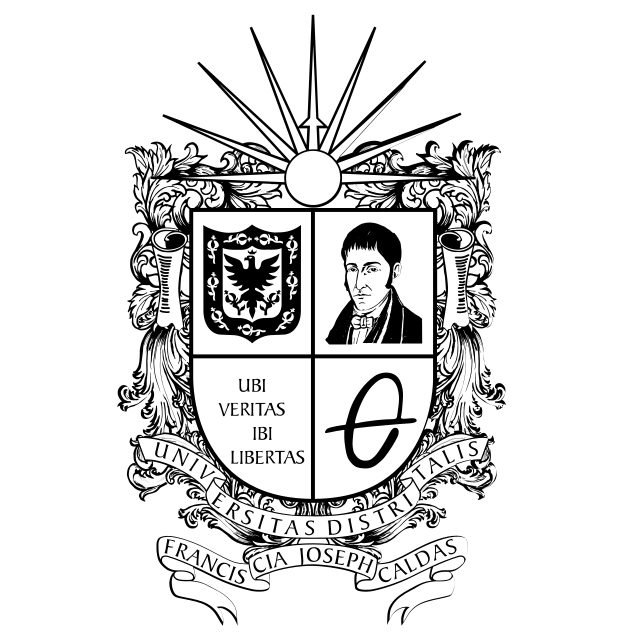
\includegraphics[width=0.2\textwidth]{Images/Escudo_UD}
            
        \large
        Universidad Distrital Francisco José De Caldas\\
        Facultad de Ingeniería\\
        Colombia, Bogotá D.C.\\
        Julio de 2025\\

        
            
    \end{center}
\end{titlepage}

\raggedbottom 

\pagenumbering{roman}
    % Contenido
\renewcommand\contentsname{\textbf{Índice}}
\tableofcontents
\setcounter{tocdepth}{2}
\newpage
    % Fíguras
\renewcommand{\listfigurename}{\textbf{Índice de figuras}}
\listoffigures
\newpage
    % Tablas
\renewcommand{\listtablename}{\textbf{Índice de tablas}}
\listoftables
\newpage

% Cuerpo
\pagenumbering{arabic}

% Incluir capítulos modularizados
\section{\large Introducción}
En Colombia, la gestión de fotocomparendos ha sido objeto de controversia debido a fallas en la transparencia y posibles manipulaciones en el proceso de registro y validación de infracciones. La falta de un sistema confiable ha generado desconfianza entre los ciudadanos, lo que evidencia la necesidad de una solución que garantice la integridad, inmutabilidad y verificabilidad de la información.

La tecnología Blockchain ha demostrado ser una alternativa eficaz para el almacenamiento seguro y descentralizado de datos, asegurando que una vez registrados, estos no puedan ser alterados sin dejar rastro. A través de contratos inteligentes, es posible automatizar la validación y el procesamiento de fotocomparendos, reduciendo la intervención humana y minimizando el riesgo de corrupción o errores administrativos.

Este trabajo propone el diseño e implementación de un prototipo basado en Blockchain para la gestión de fotocomparendos en Bogotá, con el objetivo de garantizar la transparencia del proceso. Se utilizarán contratos inteligentes para registrar cada infracción, permitiendo que cualquier actor autorizado pueda verificar su autenticidad sin necesidad de intermediarios. Mediante pruebas y simulaciones, se evaluará la viabilidad del sistema, demostrando cómo esta tecnología puede fortalecer la confianza en los procesos de control de tránsito y mejorar la eficiencia en la gestión de sanciones.

\subsection{Formulación del problema}
El sistema actual de gestión de fotocomparendos en Bogotá, enfrenta serias limitaciones en términos de transparencia, seguridad e integridad de la información, lo que genera desconfianza por parte de la ciudadanía y dificultades administrativas en su gestión. Según el Observatorio de Movilidad de Bogotá, entre enero de 2018 y agosto de 2024 se emitieron 5.575.982 comparendos, de los cuales el 48,91 \% fueron generados mediante dispositivos electrónicos de asistencia policial \parencite{ObservatorioComparendos2025}

\begin{figure}[htbp]
    \begin{flushleft}
        \textbf{Figura 1}\\
        \textit{Estadísticas de comparendos emitidos en Bogotá entre enero de 2018 y agosto de 2024}
    \end{flushleft}
    \centering
    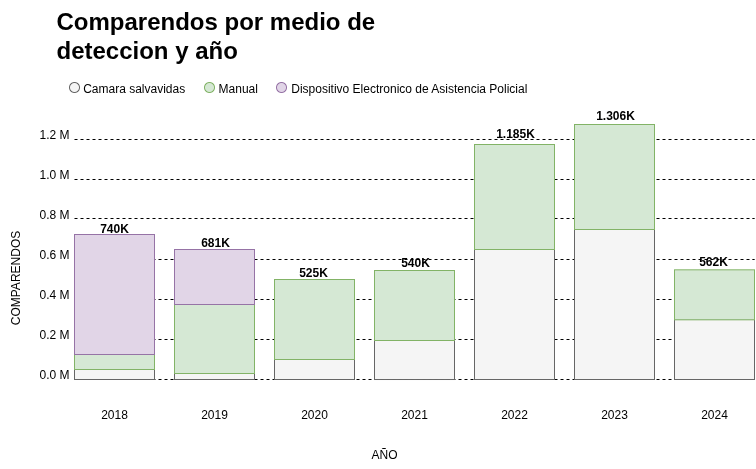
\includegraphics[width=0.8\textwidth]{Images/numComparendos.png}
    \vspace{0.5em}
    \begin{flushleft}
        \textit{Nota.} Tomado del Observatorio de Movilidad de Bogotá.
    \end{flushleft}
    \label{fig:estadisticas_comparendos}
\end{figure}

Estas cifras reflejan el papel protagónico que tienen las fotomultas en la regulación del tránsito en la ciudad, pero también resaltan la necesidad urgente de fortalecer los mecanismos de manejo, almacenamiento y verificación de evidencias.  

La ausencia de un sistema confiable y auditable que permita garantizar la inmutabilidad de los registros, así como la trazabilidad de las evidencias, ha generado un entorno donde se cuestiona la validez de las sanciones, se incrementan las quejas ciudadanas y se limita la eficiencia operativa de las entidades encargadas del control de tránsito. En este contexto, surge la necesidad de explorar tecnologías emergentes, como Blockchain e IPFS, que podrían ofrecer una solución más segura, descentralizada y transparente para la gestión de estos procesos. 

\subsection{Objetivos}
\paragraph{Objetivo General}
Desarrollar un prototipo que gestione los foto comparendos en Bogota, utilizando tecnologías como Hyperledger Fabric e InterPlanetary File System con el fin de tener una gestión segura, auditable y descentralizada del  proceso. 

\paragraph{Objetivos específicos}
\begin{itemize}
    \item Analizar el proceso actual de gestión de fotocomparendos en Bogotá, mediante la revisión de la normativa y una auditoria del sistema Fenix -El istema que actualmnte gestiona los fotocomparendos en Bogota- para identificar las vulnerabilidades y los requisitos funcionales y no funcionales (seguridad, rendimiento y auditabilidad) que el prototipo debe satisfacer, resultando en una lista de requerimientos específicos para la nueva solución.
    \item Construir el prototipo del sistema de gestión de foto comparendos, implementando la arquitectura propuesta (InterPlanetary File System para almacenamiento de imágenes y Hyperledger Fabric para el registro de transacciones), asegurando que cada transacción contenga el hash único de InterPlanetary File System y los metadatos esenciales del comparendo (fecha, hora, lugar, placa, tipo de infracción), y desarrollando una interfaz básica que permita la carga de la evidencia y la consulta/verificación de los registros en la blockchain y la imagen en InterPlanetary File System, con el fin de materializar técnicamente la solución propuesta basada en los requisitos identificados en el objetivo anterior.
    \item Evaluar la efectividad y viabilidad del prototipo desarrollado, mediante la ejecución de un plan de pruebas funcionales (verificar la correcta carga a InterPlanetary File System, el registro inmutable en el ledger, la consistencia de datos, la capacidad de verificación) y pruebas de rendimiento básicas (medir tiempos de registro y consulta) en un entorno de simulación controlado, para validar que el prototipo cumple con los requisitos clave de inmutabilidad, transparencia y seguridad.
\end{itemize} 
\section{\large Justificación}
La gestión actual de los fotocomparendos en Bogotá, centralizada en el sistema Fénix, presenta graves limitaciones de seguridad y transparencia que han erosionado la confianza pública en el proceso sancionatorio. Esta se manifiesta en un riesgo sistémico de corrupción, un fenómeno documentado tanto a nivel internacional, como el escándalo de «ticket-fixing» en Nueva York, como a nivel nacional, donde existen redes ilícitas que manipulan y eliminan comparendos en el sistema \parencite{barbaro2011ticketfixing, blogAletta, procuraduriaBucaramanga}.

La raíz de este problema reside en la arquitectura centralizada de las bases de datos tradicionales, que permite a personal interno modificar registros sin dejar un rastro auditable, comprometiendo la integridad de todo el proceso. Esta debilidad se ve agravada por las deficiencias en ciberseguridad identificadas en el \textit{Informe Final de Auditoría AC-SDM-090 de 2023}, que señala controles de acceso insuficientes y falta de monitoreo en los sistemas de la Secretaría de Movilidad \parencite{auditoriaSDM}. Estas falencias no solo incrementan el riesgo de ataques, sino que debilitan la capacidad institucional para defender la legitimidad de las sanciones impuestas.
Estas diferencias estructurales entre el modelo centralizado actual y la alternativa descentralizada se resumen en la Tabla~\ref{tab:comparacion_bd_blockchain}, evidenciando las ventajas de Blockchain en términos de seguridad, integridad y gobernanza de datos:

\begin{table}[htbp]
    \begin{flushleft}
        \textbf{Tabla 1}\\[2em]
        \textit{Comparación entre bases de datos tradicionales y blockchain para gestión de registros gubernamentales}
    \end{flushleft}
    \vspace{1em}
    \addcontentsline{lot}{table}{Tabla 1. Comparación entre bases de datos tradicionales y blockchain para gestión de registros gubernamentales}
    \centering
    \begin{tabular}{p{4.5cm} p{5.2cm} p{5.2cm}}
        \toprule
        \textbf{Característica} & \textbf{Base de Datos Convencional} & \textbf{Blockchain} \\
        \midrule
        Modelo de confianza & Se basa en un administrador central (entidad de TI) & Confianza distribuida entre múltiples nodos \\
        Inmutabilidad & Registros pueden ser modificados o eliminados por administradores & Los registros son inmutables por diseño \\
        Trazabilidad / Auditoría & Depende de la implementación y control interno & Historial completo e inalterable disponible \\
        Riesgo de corrupción interna & Alto, si hay privilegios indebidos o colusión & Bajo, no se puede alterar sin consenso de la red \\
        Seguridad criptográfica & Opcional, no siempre integrada nativamente & Integrada (firmas digitales, hashes, cifrado) \\
        Disponibilidad / tolerancia a fallos & Riesgo de puntos únicos de falla & Alta disponibilidad por replicación descentralizada \\
        Velocidad de operación & Alta velocidad en lectura/escritura & Menor velocidad, prioriza integridad y consenso \\
        \bottomrule
    \end{tabular}
    \vspace{2em}
    \begin{flushleft}
        \textit{Nota.} Elaboración propia.
    \end{flushleft}
    \refstepcounter{table}\label{tab:comparacion_bd_blockchain}
\end{table}

Frente a este escenario, la tecnología Blockchain, en conjunto con IPFS, ofrece un cambio de paradigma hacia un modelo más seguro y transparente. Como se observa en la comparación, a diferencia de un sistema centralizado donde la confianza recae en una única entidad falible, una solución Blockchain distribuye los datos en una red criptográficamente enlazada. Esto garantiza que cada registro, una vez validado, sea inmutable y verificable por todas las partes autorizadas, haciendo que cualquier intento de alteración sea computacionalmente inviable y fácilmente detectable. Se elimina así la dependencia de intermediarios y se crea una fuente única y confiable de verdad.

En síntesis, la adopción de este prototipo se justifica por su capacidad para:
\begin{itemize}
\item \textbf{Mitigar la corrupción}, al garantizar la integridad de los datos y eliminar la posibilidad de manipulación unilateral.
\item \textbf{Fortalecer la seguridad de la información}, mediante una arquitectura distribuida y tolerante a fallos.
\item \textbf{Aumentar la confianza ciudadana}, al ofrecer mecanismos transparentes y auditables para la validación de infracciones.
\item \textbf{Optimizar los procesos administrativos}, automatizando registros, auditorías y la verificación de evidencias.
\end{itemize}

Esta propuesta no solo responde a desafíos técnicos y éticos urgentes en Bogotá, sino que también se alinea con las tendencias globales en gobernanza digital (\textit{GovTech}), sentando un precedente innovador para la gestión de sanciones públicas con mayor fiabilidad y transparencia.
\section{\large Marco Teórico}
El marco conceptual y tecnologico que sustenta la propuesta del prototipo, presentan las teorías y modelos clave que justifican la selección de Blockchain e IPFS como componentes centrales, evidencian los principios inherentes de integridad, transparencia, resiliencia y auditabilidad en la gestión de evidencia digital crítica como los fotocomparendos.
\subsection{El Paradigma de la Confianza Descentralizada}
Los sistemas de información tradicionales suelen depender de intermediarios centralizados o autoridades certificadoras para validar transacciones y garantizar la fiabilidad de los registros. La teoría de los modelos de confianza descentralizada, en cambio, analiza cómo establecer y mantener la confianza en entornos distribuidos donde tales autoridades centrales están ausentes \parencite{swan2015blockchain}.

La relevancia de este modelo es fundamental para justificar el uso de la tecnología Blockchain en la gestión de fotocomparendos, ya que su propósito es precisamente reemplazar la necesidad de depositar confianza exclusiva en una única entidad para la custodia, validación e integridad de los registros. Blockchain habilita un cambio de paradigma: en lugar de confiar en un actor central, la confianza se distribuye y se deposita en la robustez del protocolo criptográfico subyacente \parencite{nakamoto2008bitcoin}, en la transparencia de las reglas del sistema y en el consenso mayoritario de los participantes de la red \parencite{antonopoulos2023mastering}. Este enfoque reduce drásticamente los puntos únicos de fallo y los vectores de corrupción asociados a la dependencia de intermediarios centralizados, quienes podrían ser comprometidos, cometer errores o actuar de manera malintencionada.

\subsection{Fundamentos de los Sistemas Distribuidos y Redes Descentralizadas}
El paradigma de la confianza descentralizada se sustenta en la teoría de los sistemas distribuidos, donde múltiples entidades autónomas, denominadas nodos, colaboran a través de una red para alcanzar un objetivo común, compartiendo tanto la carga computacional como el almacenamiento de datos \parencite{vanSteen2017}. Estos sistemas se fundamentan en principios como la distribución de recursos, la comunicación inter-nodo y mecanismos de coordinación que prescinden de intermediarios centrales \parencite{coulouris2011}.

La relevancia de esta teoría para el presente proyecto es primordial, ya que tanto Blockchain como el InterPlanetary File System (IPFS) son implementaciones nativas de sistemas distribuidos. Su adopción conjunta promueve inherentemente:
\begin{itemize}
    \item \textbf{Resiliencia:} Al eliminar puntos únicos de fallo (Single Points of Failure - SPOF).
    \item \textbf{Alta Disponibilidad:} Al permitir el acceso a datos y servicios desde múltiples nodos.
    \item \textbf{Resistencia a la Censura:} Dado que ninguna entidad individual posee control absoluto sobre la red o los datos almacenados \parencite{antonopoulos2023mastering}.
\end{itemize}

Una característica esencial de estos sistemas es su arquitectura de red \textbf{Peer-to-Peer (P2P)}, donde los participantes se conectan y comparten recursos directamente entre sí, sin necesidad de un servidor central. En una red P2P, cada nodo puede actuar simultáneamente como cliente y servidor, lo que posibilita que el registro distribuido (ledger) se mantenga sincronizado y que los archivos puedan ser recuperados desde múltiples fuentes, garantizando la integridad de la información sin depender de una autoridad central.

\subsection{Tecnologías para la Gestión Descentralizada de Evidencia}
Para materializar un sistema de gestión de fotocomparendos descentralizado, se requiere la sinergia de dos tipos de tecnologías: una para el registro inmutable de transacciones y otra para el almacenamiento verificable de la evidencia.

\subsubsection{Blockchain: Un Registro Distribuido, Inmutable y Transparente}
Blockchain es un tipo específico de Tecnología de Ledger Distribuido (DLT), un sistema de registro digital caracterizado por ser distribuido, sincronizado y asegurado criptográficamente entre múltiples participantes \parencite{narayanan2016bitcoin}. Su estructura fundamental se compone de \textbf{transacciones} —operaciones firmadas digitalmente que modifican el estado del ledger de forma permanente \parencite{antonopoulos2023mastering}— agrupadas en bloques. Cada bloque contiene un hash criptográfico que lo vincula al anterior, formando una cadena cronológica e inmutable.

La \textbf{inmutabilidad} y la \textbf{transparencia} son los beneficios centrales que esta tecnología aporta \parencite{swan2015blockchain,antonopoulos2023mastering}. La primera se logra mediante la estructura encadenada y los mecanismos de consenso distribuido (ej., Proof-of-Work \parencite{nakamoto2008bitcoin} o Proof-of-Stake \parencite{king2012ppcoin}), que hacen que la modificación de un bloque pasado sea computacionalmente prohibitiva. La segunda se habilita por la naturaleza replicada del ledger, permitiendo que actores autorizados puedan consultar y verificar la información de forma independiente. Dentro de este ecosistema, los \textbf{Smart Contracts} (Contratos Inteligentes) actúan como programas autoejecutables cuyo código define e impone automáticamente los términos de un proceso, permitiendo automatizar la gestión del ciclo de vida del comparendo \parencite{szabo1997smart, wood2014ethereum, buterin2014next}.

\paragraph{Modelos Arquitectónicos y Elección para el Prototipo.}
La tecnología Blockchain no es monolítica; existen diferentes arquitecturas:
\begin{itemize}
    \item \textbf{Públicas (Permissionless):} Abiertas a cualquier participante, priorizan la descentralización radical (ej. Bitcoin, Ethereum) \parencite{nakamoto2008bitcoin}.
    \item \textbf{Privadas:} Controladas por una única entidad, ofrecen alta eficiencia pero son centralizadas.
    \item \textbf{De Consorcio/Permisionadas (Permissioned):} Operadas por un grupo selecto de participantes autorizados. Ofrecen un equilibrio entre descentralización, rendimiento y confidencialidad, siendo la opción ideal para contextos gubernamentales y empresariales \parencite{vukolic2015quest,cachin2018architecture}.
\end{itemize}
Para este prototipo, se opta por una \textbf{implementación permisionada} (simulada con Hyperledger Fabric), permitiendo que solo entidades autorizadas operen nodos y registren transacciones, con un mecanismo de consenso eficiente (ej. Raft) adecuado para un sistema de gestión de registros.

\subsubsection{IPFS: Almacenamiento Verificable mediante Direccionamiento por Contenido}
Los ledgers de Blockchain no están optimizados para almacenar grandes volúmenes de datos (blobs), como las imágenes de los fotocomparendos \parencite{xu2019taxonomy}. Para resolver esto, se utiliza un sistema de almacenamiento descentralizado. La elección de IPFS sobre alternativas centralizadas como AWS S3 es crucial para la integridad del sistema. Mientras que en un sistema centralizado el propietario puede modificar o eliminar unilateralmente un archivo \parencite{vogels2008eventually}, IPFS opera bajo el paradigma del \textbf{direccionamiento por contenido (Content Addressing)} \parencite{benet2014ipfs, voigt2017gdpr}.

En este modelo, la identidad única de un archivo, su Content Identifier (CID), es un \textbf{hash criptográfico} derivado directamente de su contenido. Esto establece un vínculo intrínseco e inmutable: si el contenido del archivo cambia, incluso mínimamente, su CID también cambiará. IPFS es un protocolo y red P2P que utiliza este principio: divide los archivos en bloques, calcula sus hashes y permite su recuperación a través de su CID, utilizando mecanismos como DHT para localizar los nodos que los poseen \parencite{maymounkov2002kademlia, benet2014ipfs}.

\subsection{Arquitectura de la Solución: Sinergia Blockchain-IPFS con el Transacción Off-Chain}
La integración de ambas tecnologías se materializa mediante el patrón de almacenamiento \textbf{off-chain}. El flujo de trabajo es el siguiente:
\begin{enumerate}
    \item La imagen probatoria del comparendo se carga a un nodo IPFS, obteniendo su CID único.
    \item Se crea una transacción en la Blockchain (on-chain) que contiene este CID junto con los metadatos esenciales del comparendo (fecha, hora, lugar, placa).
    \item Esta transacción se valida y registra de forma inmutable en el ledger.
\end{enumerate}
Este enfoque crea un enlace criptográfico inalterable entre el registro oficial (en Blockchain) y la evidencia visual original (en IPFS). Cualquier intento de manipulación de la imagen almacenada en IPFS resultaría en un CID diferente, rompiendo explícitamente la cadena de custodia digital y haciendo que la alteración sea detectable de forma inmediata y algorítmica. La combinación de Blockchain e IPFS no solo sigue los principios de descentralización \parencite{vanSteen2017}, sino que refuerza activamente los objetivos de inmutabilidad verificable y transparencia del sistema.

\subsection{Fundamentos Criptográficos Aplicados}
La criptografía proporciona los pilares matemáticos que garantizan la seguridad, integridad y autenticidad en todo el ecosistema del prototipo \parencite{katz2020introduction}.
\begin{itemize}
    \item \textbf{Funciones Hash Criptográficas:} Son algoritmos que transforman datos en una huella digital de tamaño fijo. Sus propiedades (unidireccionalidad, resistencia a colisiones, efecto avalancha) son vitales \parencite{schneier2007applied, menezes1996handbook}. En este proyecto, se utilizan para: generar el CID en IPFS, asegurar la integridad de la cadena de bloques y crear identificadores únicos para las transacciones \parencite{benet2014ipfs, nakamoto2008bitcoin}.
    \item \textbf{Criptografía Asimétrica y Firmas Digitales:} Basada en pares de claves (pública y privada), habilita las firmas digitales \parencite{diffie2022new, rivest1978method}. Cuando un usuario autorizado registra un comparendo, utiliza su clave privada para firmar la transacción. Cualquier participante puede usar la clave pública correspondiente para verificar la firma, garantizando así la \textbf{autenticidad} y el \textbf{no repudio} de la acción \parencite{katz2020introduction}.
\end{itemize}
\section{\large Estado del Arte}  

\subsection{Blockchain para Registros Gubernamentales y Gestión de Sanciones} 

La aplicación de la tecnología Blockchain y DLT (Distributed Ledger Technology) en la administración pública ha sido un área de creciente interés, impulsada por las promesas teóricas de Inmutabilidad, Transparencia y Auditoría mejorada, fundamentales para la Confianza Descentralizada. La investigación sugiere que Blockchain puede transformar la gestión de registros oficiales, como licencias, títulos de propiedad y, potencialmente, multas o sanciones como los fotocomparendos. 

\paragraph{Análisis de Aplicación}
La capacidad de crear un registro de Transacciones criptográficamente asegurado y distribuido permite generar una pista de auditoría fiable y resistente a la manipulación. Cada registro de sanción, incluyendo sus Metadatos (fecha, hora, ubicación, tipo de infracción) y el Hash de la evidencia asociada, puede ser anclado a la cadena, proporcionando una fuente única de verdad verificable por las partes autorizadas. Esto se alinea con los principios de Sistemas Distribuidos aplicados a la gobernanza. 

\paragraph{Blockchains Públicas vs. Permisionadas}
En el contexto gubernamental, la literatura y los estudios piloto tienden a favorecer las blockchains permisionadas (o de consorcio). Si bien las blockchains públicas ofrecen máxima transparencia, las permisionadas permiten a las entidades gubernamentales controlar quién puede participar en la red (validar transacciones, acceder a datos), gestionar mejor la privacidad (crucial para datos ciudadanos) y, a menudo, ofrecer mayor rendimiento y escalabilidad. La elección impacta directamente en el modelo de Confianza Descentralizada implementado. 

\paragraph{Madurez y Barreras}
Aunque existen numerosos estudios y proyectos piloto (ej., registros de tierras en Suecia o Georgia, identidad digital en Estonia), las implementaciones a gran escala para la gestión integral de sanciones administrativas aún son limitadas. La madurez es variable. Las barreras reconocidas incluyen la complejidad técnica, la necesidad de marcos legales y regulatorios adaptados, la interoperabilidad con sistemas heredados, los costos iniciales de implementación y la adopción tanto por parte de las instituciones como de los ciudadanos. La Percepción Pública de la Tecnología Blockchain también juega un rol significativo. 

\subsection{Integración de Blockchain e IPFS para Datos Voluminosos y Verificables} 

El almacenamiento directo de datos voluminosos (como imágenes o vídeos de alta resolución) en una Blockchain es ineficiente y costoso. La literatura técnica y diversos prototipos exploran la integración de Blockchain con sistemas de Almacenamiento Direccionable por Contenido como IPFS (InterPlanetary File System) para abordar este desafío. 

\paragraph{Estado Actual} El enfoque predominante consiste en almacenar el dato voluminoso (la imagen del fotocomparendo) en IPFS, obteniendo un Hash único basado en su contenido. Este Hash IPFS, junto con otros Metadatos relevantes, se almacena en una Transacción Blockchain. Este modelo aprovecha la eficiencia de IPFS para el almacenamiento distribuido y la fortaleza de Blockchain para el registro inmutable y verificable del puntero (el Hash) y los metadatos asociados. 

\paragraph{Ventajas y Desafíos} Las ventajas logradas incluyen la verificabilidad (cualquier cambio en el archivo IPFS cambiaría su hash, invalidando el enlace en la Blockchain), la resiliencia potencial (si múltiples nodos almacenan el archivo) y el direccionamiento por contenido inherente a IPFS. Sin embargo, persisten desafíos persistentes significativos: 

\paragraph{Persistencia de Datos (Pinning)} Los datos en IPFS solo persisten mientras algún nodo los esté "pineando" (almacenando activamente). Garantizar la persistencia a largo plazo de la evidencia requiere mecanismos o servicios de pinning fiables, que pueden tener costos asociados. 

\paragraph{Disponibilidad} La recuperación del archivo depende de que los nodos que lo almacenan estén en línea y accesibles. 

\paragraph{Costos a Largo Plazo} El almacenamiento distribuido no es necesariamente gratuito, especialmente si se requieren garantías de disponibilidad y persistencia. 

\paragraph{Gestión de la Privacidad} Los datos en IPFS son típicamente accesibles públicamente si se conoce el hash. Para evidencia sensible, se requerirían capas adicionales de encriptación antes de la subida a IPFS, añadiendo complejidad. 

\subsection{Gestión de Evidencia Digital y Cadena de Custodia con DLT}

La integridad y la cadena de custodia de la evidencia digital son cruciales en procesos sancionatorios. Blockchain/DLT ofrece mecanismos basados en Criptografía Aplicada para fortalecer estos aspectos. 

\paragraph{Fortalecimiento de la Integridad y Trazabilidad} Al registrar el Hash de la evidencia digital (imagen del fotocomparendo) en una Transacción Blockchain, se crea un sello de tiempo (timestamping) inmutable y verificable. Cualquier intento posterior de modificar la evidencia original resultaría en un hash diferente, lo que permitiría detectar fácilmente la manipulación. La secuencia de transacciones en la Blockchain proporciona una trazabilidad auditable del ciclo de vida de la evidencia (captura, registro). 

\paragraph{Comparación y Valor Añadido} En comparación con los sistemas tradicionales (bases de datos centralizadas, logs de servidor), que pueden ser susceptibles a alteraciones internas o fallos únicos, la DLT aporta un valor añadido significativo al distribuir la confianza y hacer que la manipulación sea computacionalmente inviable (principio de Inmutabilidad). Esto refuerza la Confianza Descentralizada en la validez de la evidencia presentada, reduciendo potenciales disputas. 

\paragraph{Estándares Emergentes} En el ámbito de la tecnología blockchain, observamos la consolidación de estándares emergentes en diversas áreas, que representan un consenso práctico y técnico en ausencia de normas formales universalmente ratificadas. 

Un área clave es la Seguridad de Smart Contracts. Para construir confianza y fiabilidad en las aplicaciones descentralizadas (dApps) y mitigar vulnerabilidades, se están adoptando ampliamente prácticas que funcionan como estándares de facto: 
\begin{itemize}
    \item \textbf{Auditorías y Listas de Chequeo:} Metodologías promovidas por firmas especializadas como ConsenSys Diligence, Trail of Bits y OpenZeppelin se han vuelto habituales. 
    \item \textbf{Patrones de Diseño Seguro:} Se aplican convenciones como Checks-Effects-Interactions y el uso de proxies actualizables (UUPS, Transparent Proxy), aunque estos patrones continúan evolucionando. 
    \item \textbf{Estándares de Reporte de Vulnerabilidades:} Propuestas como las EIPs (Ethereum Improvement Proposals) relacionadas con la seguridad ayudan a estandarizar la comunicación de fallos.
\end{itemize}

Otra área fundamental donde emergen estándares es la Gestión de Evidencia Digital y Cadena de Custodia mediante Blockchain/DLT. Aunque todavía no existe una norma global única (como un estándar ISO específico para esta aplicación), sí se está formando un fuerte consenso técnico sobre los principios tecnológicos clave para asegurar la integridad y fiabilidad:

\begin{itemize}
    \item \textbf{Hashing Criptográfico:}El uso de funciones hash para generar una huella digital única e infalsificable de la evidencia (como el CID en IPFS) es la práctica estándar para garantizar la integridad y detectar manipulaciones \parencite{benet2014ipfs}. 
    \item \textbf{Timestamping Inmutable:} Registrar el hash de la evidencia y sus metadatos en una transacción blockchain proporciona una marca de tiempo segura e inalterable, estableciendo una prueba fehaciente del momento del registro \parencite{nakamoto2008bitcoin}. 
    \item \textbf{Registro en Ledger Distribuido (DLT):} Utilizar la DLT como el libro contable distribuido para estos registros es el mecanismo reconocido para lograr inmutabilidad, transparencia controlada y auditabilidad \parencite{swan2015blockchain}, superando las limitaciones de las bases de datos centralizadas.
\end{itemize}

\subsection{Funcionamiento de los Fotocomparendos en Bogotá: Mecanismos, Regulación e Impacto} 
El sistema de fotocomparendos en Bogotá (FENIX) representa un modelo tecnológico y regulatorio diseñado para mejorar la seguridad vial mediante la detección automatizada de infracciones de tránsito \parencite{mintransporte2023}. Basado en cámaras de fotodetección ubicadas en zonas autorizadas por el Ministerio de transporte, este sistema combina vigilancia electrónica, validación humana y marcos legales específicos para sancionar conductas de riesgo \parencite{supertransporte2021}. Desde su implementación, ha logrado reducir siniestros en puntos críticos, aunque enfrenta desafíos técnicos y jurídicos. A continuación, se detalla su operación, criterios de aplicación y marco legal que lo regula \parencite{mintransporte2023}.

\paragraph{Marco Legal y Regulatorio} La implementación de fotocomparendos en Bogotá se sustenta en la Ley 1843 de 2017 \parencite{ley1843} y su reglamentación mediante resoluciones como la Resolución 20203040011245 \parencite{resolucion11245}. Estos instrumentos establecen cuatro criterios para instalar cámaras: 

\begin{enumerate}
    \item \textbf{Siniestralidad:}Ubicación en zonas con alto índice de accidentes. 
    \item \textbf{Prevención:} Disuasión de conductas peligrosas. 
    \item \textbf{Movilidad: } Optimización del flujo vehicular.
        \item \textbf{Historial de infracciones:} Enfoque en corredores con recurrentes violaciones.
\end{enumerate}

Adicionalmente, las autoridades deben garantizar la visibilidad de los dispositivos, señalizando su presencia al menos 500 metros antes de su ubicación \parencite{ley1843}, y cumplir con planes de seguridad vial alineados con políticas distritales. La Secretaría Distrital de Movilidad (SDM) ha enfrentado cuestionamientos legales, como los señalados por la Personería en 2018 \parencite{sdm2023camaras}.

\paragraph{Proceso Operativo de los Fotocomparendos} La implementación de fotocomparendos en Bogotá se sustenta en la Ley 1843 de 2017 \parencite{ley1843} y su reglamentación mediante resoluciones como la Resolución 20203040011245

\paragraph{Proceso Operativo de los Fotocomparendos }
\paragraph{Detección y Captura de Infracciones }
Las cámaras de fotodetección en Bogotá se clasifican en dos tipos \parencite{supertransporte2021, mintransporte2023}: 

\begin{itemize}
    \item \textbf{Automáticas: }Monitorean velocidades, semáforos en rojo y restricciones como pico y placa.
    \item \textbf{Semiautomáticas:}Vigilan bloqueos de calzadas, paradas prohibidas y recolección irregular de pasajeros.
\end{itemize}

Estos dispositivos, instalados en corredores de alta accidentalidad como la Avenida NQS o la Calle 100, capturan imágenes o videos que incluyen matrícula, fecha, hora y ubicación GPS14. Por ejemplo, en 2025, un conductor que exceda el límite de 50 km/h en la Avenida Boyacá será registrado por cámaras previamente señalizadas. 

\paragraph{Validación y Notificación }
Una vez detectada una presunta infracción, las pruebas se envían a un centro de análisis de la SDM, donde agentes de tránsito verifican:

\begin{itemize}
    \item Legibilidad de la matrícula. 
    \item Contexto de la violación (ejemplo: si un semáforo en rojo fue respetado).
    \item Datos del vehículo en el RUNT (Registro Único Nacional de Tránsito).
\end{itemize}

Tras validar la infracción, se genera un comparendo electrónico notificado al propietario del vehículo mediante correo certificado o plataformas digitales. El plazo máximo para emitir la sanción es de 10 días hábiles desde la detección, seguido de 3 días para su notificación. Si el domicilio registrado está desactualizado, el infractor podría no recibir la notificación, lo que no exime el pago \parencite{ley1843}. 

\paragraph{Tecnología y Transparencia }
El sistema combina: 
\begin{itemize}
    \item \textbf{Cámaras de última generación: }Equipadas con sensores de velocidad Lidar y visión nocturna. 
    \item \textbf{Plataforma de análisis IA: }Algoritmos que descartan falsos positivos (ejemplo: ambulancias en emergencia). 
        \item \textbf{Integración con RUNT:}Verificación instantánea de documentos como SOAT o tarjeta de operación.
\end{itemize}

Los datos se almacenan en servidores con cifrado AES-256, accesibles solo para funcionarios autorizados mediante autenticación biométrica.

\paragraph{Problemas Operativos }
\begin{itemize}
    \item \textbf{Notificaciones fallidas: }Errores en direcciones del RUNT causan sanciones no recibidas, acumulando intereses moratorios. 
    \item \textbf{Latencia en validaciones:  }En horas pico, el volumen de infracciones puede retrasar procesamientos hasta 72 horas.
\end{itemize}

\paragraph{Cuestionamientos Legales }
En 2018, la Personería de Bogotá identificó que el 15\% de las cámaras operaban sin autorización ministerial durante un periodo de transición legal. La SDM rectificó esta situación en 2019, regularizando todos los dispositivos bajo la Resolución 20203040011245 de 2020 \parencite{secretaria_movilidad2023}. 

\subsection{Aplicaciones Específicas en Gestión de Tráfico e Infracciones} 

Al revisar las Aplicaciones de Blockchain en la Gestión de Tráfico, Infracciones y Fotocomparendos, se observa que, si bien hay discusiones teóricas \parencite{yousfi2022its}, propuestas conceptuales \parencite{chen2024blockchain} y hasta una joven PYME española, las implementaciones prácticas que integren el flujo completo descrito en el prototipo (captura -> IPFS -> Blockchain -> Verificación -> Pago Automatizado con Billetera Digital) son escasas y se encuentran en fase de propuesta o son parciales \parencite{omar2024srtm,choquevilca2024blockchain}. 

\paragraph{Análisis de Existencia}
La literatura existente se centra más en componentes aislados \parencite{yousfi2022its}, uso de blockchain para registros vehiculares \parencite{ManiJosephP2023SmartAS}, seguros \parencite{dutta2023solution}, o gestión genérica de multas \parencite{omar2024srtm}, pero raramente combinando el almacenamiento de evidencia en IPFS con la automatización del pago vía billetera digital específicamente para fotocomparendos.

\paragraph{Arquitecturas y Resultados} Dada la escasez de implementaciones completas reportadas \parencite{AnandSingh_ProjectReport_Year,juit2024traffic}, es difícil generalizar sobre arquitecturas dominantes o resultados concretos para este caso de uso tan específico. Los estudios existentes a menudo se limitan a explorar la viabilidad teórica o a implementar módulos parciales \parencite{choquevilca2024blockchain}.

\paragraph{Lecciones Aprendidas:} La principal lección aprendida de áreas adyacentes es la importancia de abordar no solo los desafíos técnicos (Zheng et al., 2018) sino también los regulatorios, de gobernanza y de adopción (Tan et al., 2022). La ausencia de soluciones integrales reportadas para el flujo completo de gestión de fotocomparendos representa una brecha significativa en la aplicación práctica de estas tecnologías combinadas.

El análisis del estado del arte revela avances significativos, pero también limitaciones claras: 
  

\subsection{Avances Significativos} 

La tecnología Blockchain ha demostrado su potencial para crear registros gubernamentales más inmutables, transparentes y auditables. (Balcerzak et al., 2022; Meroni et al., 2023) 

La integración Blockchain + IPFS es una solución técnicamente viable y reconocida para gestionar datos voluminosos referenciados desde una cadena de bloques, mejorando la verificabilidad (Adel et al., 2023; Mishra et al., 2024). 

DLT ofrece mejoras sustanciales para la integridad y trazabilidad de la evidencia digital (Thanasas et al., 2025). 

Existen mecanismos (billeteras digitales, smart contracts, stablecoins) para habilitar pagos digitales automatizados en ecosistemas blockchain \parencite{antonopoulos2023mastering}.

\subsection{Limitaciones Identificadas} 
\paragraph{Madurez e Integración:}
Muchas aplicaciones gubernamentales de Blockchain son pilotos aislados (Zheng et al., 2018; Li et al., 2021). Falta integración entre sistemas y con procesos completos. 

\paragraph{Desafíos Técnicos: }
La persistencia y gestión a largo plazo de datos en IPFS (pinning), la escalabilidad de algunas blockchains y la seguridad/fiabilidad de los oráculos para Smart Contracts siguen siendo áreas de desarrollo activo (Zheng et al., 2018). 

\paragraph{Adopción y Regulación:}
La adopción de billeteras digitales para pagos gubernamentales, el uso de criptoactivos/stablecoins y la claridad legal sobre smart contracts en el sector público son obstáculos importantes (Tan et al., 2022).

\paragraph{Política de Reserva de Información:}
 La Municipalidad Provincial del Cusco mantiene una política de reserva de información que restringe la divulgación completa de los datos almacenados en su base de datos. Esta política limita el acceso y la difusión de ciertos datos, lo que puede afectar la transparencia y la capacidad de realizar un análisis exhaustivo \parencite{choquevilca2024blockchain}.

\paragraph{Actualización de Datos:}
La actualización de los datos almacenados en la base de datos es un proceso que requiere tiempo. Dada la naturaleza progresiva de este proceso, que depende de la cantidad de datos que se agregan diariamente, la actualización completa de los datos con el sistema que se desarrollará puede llevar un tiempo considerable \parencite{choquevilca2024blockchain}. 

\paragraph{Aplicación Específica:}
Existe una notable ausencia de soluciones documentadas que implementen el flujo completo e integrado (captura de imagen -> subida a IPFS -> registro en Blockchain -> verificación vía app -> pago automático desde billetera digital) específicamente para la gestión de fotocomparendos. \parencite{yousfi2022its, chen2024blockchain}


\paragraph{Verificación Participativa:}
Los sistemas actuales raramente permiten que el ciudadano verifique independientemente la autenticidad e integridad de la evidencia presentada contra ellos, limitando los beneficios de transparencia inherentes a blockchain. 

\paragraph{Adopción en Bogotá:}
 La literatura muestra una escasez notable de implementaciones o estudios piloto en contextos latinoamericanos, donde factores como confianza institucional, infraestructura tecnológica y marcos regulatorios presentan desafíos particulares. \parencite{choquevilca2024blockchain, rezabala2025blockchain}

\subsection{Novedad y Relevancia del Prototipo} 
La(s) brecha(s) específica(s) que este prototipo busca abordar es precisamente la falta de una solución integrada y de extremo a extremo para la gestión de fotocomparendos utilizando la sinergia de Blockchain, IPFS y pagos automatizados, como se evidencia en la revisión de la literatura existente \parencite{yousfi2022its,AnandSingh_ProjectReport_Year}
La novedad principal radica en la integración holística de todo el flujo propuesto. Mientras que los componentes individuales han sido explorados por separado (Adel et al., 2023; Mishra et al., 2024) o en otros contextos (Mani Joseph P, 2023; Dutta et al., 2023), este prototipo propone conectarlos en una secuencia lógica y automatizada para este caso de uso particular. 

Aborda la brecha de aplicación específica, llevando los conceptos teóricos \parencite{swan2015blockchain, antonopoulos2023mastering} y las soluciones parciales existentes \parencite{choquevilca2024blockchain} a un dominio concreto (fotocomparendos en Bogotá) con un proceso completo. 

\subsection{La relevancia del prototipo se justifica por su potencial para:} 
Mejorar la transparencia y confianza en el proceso de fotocomparendos, evidencia verificable e inmutable (Meroni et al., 2023; Thanasas et al., 2025). 

Aumentar la eficiencia operativa mediante la automatización del registro, verificación y pago. 

Reducir disputas y costos asociados a la gestión manual y a la falta de confianza en la evidencia. 

Explorar un modelo innovador de pago automatizado condicional basado en la verificación en Blockchain. 

 \subsection{Bibliometrix}
 \paragraph{Producción Científica por Países (Mapa y Gráfico de Líneas) }
 
 \textbf{Descripción General:} Esta gráfica se compone de dos partes. La primera es un mapa mundial que utiliza una escala de color para representar la cantidad de producción científica por país. Las tonalidades más oscuras generalmente indican una mayor producción. La segunda parte es un gráfico de líneas que muestra la evolución de la producción científica (en artículos) a lo largo de los años para un conjunto específico de países. 
\paragraph{Mapa Mundial:}
El mapa muestra la distribución global de la producción científica en el área de estudio. Se observa una concentración significativa de publicaciones en países como Brasil, lo que sugiere un interés y actividad investigadora importante en Latinoamérica. Otros países con una producción notable incluyen México y España. Es importante notar que algunas regiones muestran una menor actividad, lo que podría indicar diferencias en el enfoque de investigación, financiamiento o acceso a recursos. 
\section{Alcance}

\subsection{Enfoque y delimitación geográfica}
Este trabajo se circunscribe al proceso de generación, gestión y verificación de \textbf{multas de tránsito automatizadas (fotomultas)} emitidas por la Secretaría Distrital de Movilidad de Bogotá.  Se excluyen deliberadamente:
\begin{itemize}
  \item Multas impuestas de forma presencial por agentes de tránsito.
  \item Procesos sancionatorios de otras ciudades o entidades territoriales.
  \item Funcionalidades de recaudo y pasarelas de pago (solo se registra el estado del pago, no se procesa el pago en sí).
\end{itemize}

\subsection{Componentes del prototipo}
El prototipo aborda los siguientes módulos funcionales:

\begin{enumerate}
  \item \textbf{Registro inmutable de la infracción}  
        Captura de metadatos (placa, fecha, hora, ubicación y tipo de infracción) y publicación del identificador de la evidencia en la \emph{blockchain} (Hyperledger Fabric).
  \item \textbf{Almacenamiento descentralizado de evidencias}  
        Carga de la imagen o video de la fotomulta en IPFS y obtención de su \emph{hash}.
  \item \textbf{Verificación pública}  
        Servicio de consulta que permite contrastar el hash guardado en la cadena con el archivo almacenado en IPFS.
  \item \textbf{Gestión del ciclo de vida de la multa}  
        Estados: \textsf{Generada} $\rightarrow$ \textsf{Notificada} $\rightarrow$ \textsf{En apelación} $\rightarrow$ \textsf{Pagada} $\rightarrow$ \textsf{Cerrada}.  
        Cada transición queda registrada mediante eventos de contrato inteligente.
  \item \textbf{Interfaz mínima}  
        Panel Web para: (i) agentes que registran la infracción y (ii) ciudadanos que consultan la autenticidad y el estado de su fotomulta.
\end{enumerate}

\subsection{Fuera del alcance}
\begin{itemize}
  \item Integración completa con sistemas legados del RUNT o SIMIT; se simula mediante datos de prueba.
  \item Implementación de un modelo económico (tarifas de gas, costos operativos reales).
  \item Implementación de algoritmos de detección automática de infracciones (visión por computador).  
        Se parte de que la cámara ya detectó la infracción y generó la evidencia.
\end{itemize}

\subsection{Entregables}
\begin{itemize}
  \item Contrato inteligente en Solidity (o «chaincode» en Go, según la red seleccionada) con pruebas unitarias.
  \item Script de despliegue de red Hyperledger Fabric e instalación de IPFS local.
  \item Aplicación Web de demostración (\emph{frontend} ligero) conectada a los servicios anteriores.
  \item Manual técnico que documenta la arquitectura y el flujo de datos.
  \item Informe de resultados de las pruebas funcionales y de rendimiento básico.
\end{itemize}

\subsection{Criterios de éxito}
\begin{enumerate}
  \item Tiempo medio de publicación de una infracción $\leq$ 3 s en entorno de laboratorio.
  \item Coincidencia 100 \% entre el hash almacenado en la cadena y la evidencia recuperada desde IPFS.
  \item Trazabilidad completa del historial de estados para al menos 50 multas de prueba.
  \item Ausencia de fallos críticos en pruebas de carga con 10 transacciones concurrentes.
\end{enumerate}

\section{Limitaciones del Prototipo}
Es fundamental reconocer que, como prototipo desarrollado en un contexto académico, el presente estudio presenta ciertas limitaciones que definen el alcance de sus conclusiones y delinean claras oportunidades para futuras investigaciones. Las principales limitaciones son:

\begin{enumerate}
    \item \subsection{Entorno de Validación}
    \begin{itemize}
        \item \textbf{Validación en Entorno de Laboratorio:} El prototipo fue diseñado, desplegado y evaluado en un entorno de simulación controlado. No se sometió a pruebas en una infraestructura productiva real con la carga de transacciones y el volumen de usuarios que gestiona actualmente la Secretaría de Movilidad. Por lo tanto, su rendimiento, estabilidad y escalabilidad bajo condiciones de estrés real aún no han sido cuantificados.
        \item \textbf{Uso de Datos Simulados:} Debido a estrictas normativas de privacidad y protección de datos personales que impiden el acceso a información real de ciudadanos y vehículos, todas las pruebas se realizaron con datos sintéticos. Esto implica que el prototipo no fue expuesto a la variabilidad, inconsistencias y casos atípicos que caracterizan a los datos del mundo real, lo cual podría influir en la lógica de negocio y en el manejo de errores en un entorno de producción.
        \item \textbf{Suposiciones sobre la Calidad de la Evidencia:} El sistema asume que las evidencias fotográficas (imágenes de fotocomparendos) son capturadas con una calidad suficiente para su procesamiento. No se implementaron ni probaron mecanismos para manejar escenarios con imágenes de baja resolución, borrosas o con obstrucciones, que son comunes en la operación real.
    \end{itemize}

    \item \subsection{Integración y Comparación con Sistemas Existentes}
    \begin{itemize}
        \item \textbf{Integración Simulada con Sistemas Externos:} La interacción con plataformas gubernamentales clave como el RUNT y el SIMIT fue simulada a través de APIs de prueba (mocks). No se abordaron los desafíos técnicos y burocráticos de una integración real, como los protocolos de comunicación, los tiempos de respuesta, la disponibilidad de los servicios y los posibles cuellos de botella.
        \item \textbf{Ausencia de Benchmarking Directo con el Sistema Actual (Fénix):} La falta de acceso al código fuente y a la arquitectura interna del sistema Fénix impidió realizar una comparación cuantitativa y directa en términos de rendimiento, costos operativos o eficiencia de procesos. El análisis comparativo se basó en las características conceptuales de ambas arquitecturas (centralizada vs. descentralizada).
    \end{itemize}

    \item \subsection{Aspectos Técnicos y de Escalabilidad}
    \begin{itemize}
        \item \textbf{Proyección de Costos como Escenario de Referencia:} Los costos de infraestructura y desarrollo estimados corresponden a un escenario de referencia. Los costos reales en un despliegue a gran escala podrían variar considerablemente dependiendo de factores como el número de nodos en la red, el volumen de almacenamiento en IPFS, el tráfico de red y la estrategia de persistencia de datos (pinning) que se adopte.
        \item \textbf{Estrategia de Persistencia en IPFS:} Para que la evidencia digital permanezca disponible a largo plazo en IPFS, es necesario que al menos un nodo la mantenga ``pineada''. El prototipo no implementa una política de pinning distribuida y resiliente, lo cual sería un requisito crítico para garantizar la cadena de custodia digital en un sistema de producción.
    \end{itemize}

    \item \subsection{Seguridad y Robustez}
    \begin{itemize}
        \item \textbf{Ausencia de Pruebas de Seguridad Ofensivas:} El alcance del proyecto no incluyó la realización de auditorías de seguridad formales sobre los contratos inteligentes (chaincode) ni pruebas de penetración (pentesting) sobre la aplicación web. Aunque se siguieron buenas prácticas de desarrollo, no se ha verificado formalmente la resistencia del sistema ante ataques maliciosos especializados.
    \end{itemize}
\end{enumerate}
\section{Metodología}

La realización de este proyecto se estructuró bajo un enfoque metodológico dual, diseñado para abordar tanto los requerimientos de una investigación aplicada como las particularidades del desarrollo de una solución tecnológica innovadora. A continuación se describen: el enfoque metodológico de investigación, la selección y justificación de la pila tecnológica, y el modelo de desarrollo de software utilizado para construir el prototipo.

\subsection{Enfoque metodológico de investigación}

Este trabajo se enmarca en una investigación aplicada, orientada a resolver un problema práctico y concreto: las deficiencias de integridad, transparencia y confianza en el sistema actual de gestión de fotocomparendos en Bogotá. Además, adopta un enfoque descriptivo, ya que se detallan las características, arquitectura y funcionamiento de un sistema descentralizado basado en Blockchain e IPFS, estableciendo un caso de estudio sobre la aplicación de estas tecnologías en el sector público.

\subsection{Selección y justificación de la pila tecnológica}

Una fase crítica fue la selección de las tecnologías de registro distribuido (DLT) que servirían como pilar del sistema. La decisión impacta directamente en:

\begin{itemize}
    \item Privacidad de datos personales (Ley 1581 de 2012).
    \item Escalabilidad ante $\sim$457.000 comparendos semestrales.
    \item Costos operativos predecibles (sin criptomonedas volátiles).
    \item Modelo de gobernanza institucional.
\end{itemize}

La arquitectura del prototipo es híbrida:
\begin{itemize}
    \item \textbf{Capa privada (permisionada):} gestión interna y datos sensibles.
    \item \textbf{Capa pública (blockchain):} verificación ciudadana sin intermediarios.
\end{itemize}

\subsubsection{Capa privada: Hyperledger Fabric}

Para la capa privada se seleccionó Hyperledger Fabric tras un análisis comparativo.

\begin{table}[H]
\centering
\small
\caption{Comparativo plataformas DLT para la gestión de fotocomparendos}
\begin{tabular}{p{2.4cm}p{2.2cm}p{2cm}p{2cm}p{2cm}p{2cm}}
\toprule
\textbf{Criterio} & \textbf{Hyperledger Fabric} & \textbf{Ethereum} & \textbf{Corda} & \textbf{Solana} & \textbf{Polygon} \\
\midrule
Tipo de red & Permisionada & Pública & Permisionada & Pública & Pública \\
Consenso & Raft / BFT & PoS & Notario & PoH + PoS & PoS \\
TPS & 2.000–20.000 & $\sim$30 & $\sim$1.000 & 65.000+ & 7.000+ \\
Privacidad & Alta$^{(1)}$ & Nula & Alta (P2P) & Nula & Nula \\
Smart contracts & Go, Java, Node.js & Solidity & Kotlin/Java & Rust/C & Solidity \\
Control de acceso & PKI / Roles & Abierto & Identidad & Abierto & Abierto \\
Moneda nativa & No & ETH & No & SOL & MATIC \\
Costo / tx & Sin gas & Gas variable & Sin gas & Muy bajo & Muy bajo \\
Madurez Gob. & Alta & Media & Alta (banca) & Baja (DeFi) & Media \\
\bottomrule
\end{tabular}
\vspace{2pt}
\footnotesize
$^{(1)}$ Canales privados y "Private Data Collections".\\
$^{(2)}$ Casos en Estonia, Suecia, Canadá y registros gubernamentales.
\label{tab:dlt_smart}
\end{table}

\textbf{Razones de elección de Hyperledger Fabric:}

\begin{itemize}
    \item \textbf{Privacidad y confidencialidad:} canales y colecciones privadas permiten segmentar la información, garantizando que solo entidades autorizadas (agentes, auditores) accedan a datos sensibles, cumpliendo la Ley 1581 de 2012.
    
    \item \textbf{Rendimiento:} 2 000–20 000 TPS, suficiente para el volumen de Bogotá sin cuellos de botella.
    
    \item \textbf{Sin costos de gas:} elimina volatilidad y complejidad, crítico para presupuestos gubernamentales.
    
    \item \textbf{Control de acceso granular:} PKI + roles definidos internamente (admin, agente, auditor, ciudadano).
\end{itemize}

\textbf{Descarte de alternativas:}
\begin{itemize}
    \item \textbf{Ethereum / Solana / Polygon:} públicas $\Rightarrow$ exposición total de datos y costos variables.
    \item \textbf{Corda:} orientada a finanzas; menor flexibilidad para evidencias fotográficas heterogéneas.
\end{itemize}

\subsubsection{Capa pública: Ethereum}

Para la verificación ciudadana se eligió Ethereum (testnet Sepolia) por:

\begin{itemize}
    \item \textbf{Máxima transparencia:} cualquier persona puede verificar metadatos sin permisos.
    
    \item \textbf{Ecosistema maduro:} mayor comunidad, herramientas (Ethers.js, Hardhat) y estándares (ERC-20, ERC-721).
    
    \item \textbf{Costo controlado:} solo se publican hashes y metadatos no sensibles, minimizando gastos de gas.
\end{itemize}

\subsection{Metodología de desarrollo de software: modelo por prototipos}

Para la construcción del sistema, se seleccionó el \textbf{Modelo de Desarrollo por Prototipos} (\textit{Prototyping Model}). Esta elección metodológica fue estratégica y se fundamenta en las características inherentes al proyecto.

\subsubsection{Justificación de la elección}

La adopción de este modelo iterativo responde a tres factores cruciales:

\begin{enumerate}
    \item \textbf{Naturaleza Innovadora y Riesgo Tecnológico:} El proyecto combina tecnologías emergentes como Blockchain (Hyperledger Fabric y Ethereum) e IPFS en un dominio gubernamental donde no existían precedentes locales de una integración similar. La alta incertidumbre sobre el rendimiento, la seguridad de los contratos inteligentes y la viabilidad de la sincronización entre redes heterogéneas requería una validación temprana para mitigar riesgos técnicos fundamentales.
    
    \item \textbf{Requisitos Evolutivos:} Los requisitos funcionales y no funcionales de un sistema de esta naturaleza están sujetos a cambios, tanto por la evolución de la tecnología como por posibles ajustes en el marco normativo de las sanciones de tránsito. El enfoque por prototipos ofrece la flexibilidad necesaria para adaptar la solución de forma ágil a medida que se profundiza el entendimiento del problema.
    
    \item \textbf{Validación Temprana de Conceptos:} Era imperativo demostrar la hipótesis central del proyecto —que la combinación de Blockchain e IPFS puede garantizar la inmutabilidad y verificabilidad de la evidencia digital— antes de invertir recursos en el desarrollo de una plataforma completa. El prototipo sirvió como una prueba de concepto funcional para validar esta premisa.
\end{enumerate}

\subsubsection{Fases del proceso de desarrollo}

El ciclo de vida del desarrollo siguió las fases iterativas del modelo de prototipos, adaptadas a los objetivos específicos del proyecto, como se describe en la Tabla~\ref{tab:fases_prototipos}.

\begin{table}[h]
\centering
\caption{Fases del Modelo de Prototipos Aplicado al Proyecto}
\label{tab:fases_prototipos}
\begin{tabular}{|p{3cm}|p{5cm}|p{6cm}|}
\hline
\textbf{Fase} & \textbf{Descripción} & \textbf{Aplicación en el Proyecto} \\ \hline
\textbf{1. Requisitos Iniciales} & Recopilación de los requisitos funcionales básicos y esenciales del sistema. & Se definieron las funcionalidades mínimas viables: registro inmutable de multas, almacenamiento de evidencia en IPFS, consulta pública y un mecanismo para la verificación de integridad. \\ \hline
\textbf{2. Construcción del Prototipo} & Desarrollo rápido de una versión funcional reducida que implementa los requisitos iniciales. & Se implementó un prototipo funcional que incluía un Smart Contract en una red local de Ethereum, una API REST para la comunicación y un frontend básico para la interacción del usuario. \\ \hline
\textbf{3. Evaluación del Prototipo} & Validación del prototipo mediante pruebas internas para evaluar su funcionalidad y alineación con los objetivos. & Se ejecutó un plan de pruebas exhaustivo (detallado en el Capítulo 9) para validar la inmutabilidad de los registros, la integridad de la evidencia y la usabilidad de la interfaz con datos simulados. \\ \hline
\textbf{4. Refinamiento e Iteración} & Ajuste y mejora del prototipo basándose en los hallazgos de la evaluación. & Con base en los resultados, se optimizó el consumo de gas del Smart Contract, se mejoraron las validaciones de la API y se refinó la arquitectura para incorporar la capa privada con Hyperledger Fabric. \\ \hline
\textbf{5. Documentación Final} & Una vez validado el concepto, se documenta la arquitectura final y se proponen los siguientes pasos. & Se consolidó el diseño de la arquitectura híbrida final y se elaboró un \textit{roadmap} detallado para una eventual implementación en un entorno de producción. \\ \hline
\end{tabular}
\end{table}

\subsubsection{Ventajas y limitaciones del enfoque}

La metodología por prototipos ofreció ventajas estratégicas determinantes para el éxito del proyecto, entre las que destacan la \textbf{validación temprana de la arquitectura híbrida}, la \textbf{mitigación de riesgos técnicos} relacionados con el rendimiento de IPFS y la \textbf{reducción de costos} al permitir ajustes antes de la fase final de desarrollo.

No obstante, es importante reconocer las limitaciones inherentes a este enfoque en el contexto de este trabajo:

\begin{itemize}
    \item \textbf{Rendimiento no representativo:} El prototipo fue evaluado en un entorno de laboratorio controlado, por lo que su rendimiento no refleja las condiciones de una red pública con alta carga transaccional.
    
    \item \textbf{Gestión de expectativas:} Una versión funcional puede generar expectativas en los usuarios de que el sistema está casi terminado, cuando aún requiere fases críticas de seguridad y optimización.
    
    \item \textbf{Disciplina de desarrollo:} Se requirió una disciplina estricta para asegurar que el código del prototipo, concebido para validación, no se promoviera a un entorno de producción sin pasar por procesos formales de auditoría y refactorización.
\end{itemize}

En conclusión, la metodología por prototipos fue fundamental para navegar la complejidad e incertidumbre del proyecto. Permitió demostrar de manera empírica que una arquitectura descentralizada es una solución técnica viable y socialmente pertinente para fortalecer la confianza en la gestión de fotocomparendos en Bogotá. 
\subsection{Introducción a los artefactos técnicos del diseño}
Con el fin de estructurar de manera clara el desarrollo de la solución propuesta, en esta sección se presentan los principales artefactos utilizados durante la etapa de diseño. Estos elementos permiten representar gráficamente tanto la lógica de funcionamiento como la arquitectura del sistema, sirviendo como guía para la implementación y posterior validación del prototipo.

El conjunto de diagramas que se incluye responde a la necesidad de modelar distintos aspectos del sistema. Por un lado, se usan diagramas de casos de uso para identificar las funcionalidades clave desde la perspectiva del usuario. Por otro, los diagramas de clases permiten definir la estructura del software, mientras que los diagramas de despliegue muestran cómo se distribuyen los componentes en el entorno tecnológico. Además, se incluyen diagramas de flujo que describen el comportamiento del sistema ante eventos específicos, facilitando la comprensión de su dinámica interna.

Cada uno de estos artefactos está alineado con los objetivos del proyecto y fue elaborado considerando tanto las necesidades funcionales como las características propias de las tecnologías involucradas, en particular el uso de Blockchain e IPFS. De esta forma, se busca garantizar coherencia técnica en el diseño y establecer una base sólida para el desarrollo e implementación de la solución.

\section{Diseño del Prototipo }

Se hace mencion que apesar que la documentacion para elaborar el software esta en español, es un estandar el escribir codigo en ingles por tanto para mantener coherencia los diagramas mostrados a continuacion se usara este idioma para los nombres de las variables, funciones y clases.
\subsection{Definición de Requisitos:  }
    
\begin{enumerate}
    \item \textbf{Datos sobre infracciones de tráfico:} La captura de datos detallados sobre infracciones de tráfico, como la hora de la infracción, las coordenadas GPS, el tipo de infracción, los datos de identificación del vehículo e imágenes o vídeos, garantiza que cada incidente se documenta exhaustivamente. Este registro exhaustivo proporciona transparencia y responsabilidad, ya que los datos son inmutables y a prueba de manipulaciones una vez almacenados en la cadena de bloques. La inclusión de pruebas mediáticas refuerza aún más la credibilidad y verificabilidad de cada infracción, haciendo que los registros sean sólidos a efectos legales y administrativos. 
    \item \textbf{Información sobre el conductor:} Asociar las infracciones de tráfico a conductores concretos utilizando su dirección Ethereum (clave pública), los datos KYC si es necesario, y los números de identificación del conductor permite un seguimiento y una rendición de cuentas precisos. Esta vinculación permite al sistema personalizar el seguimiento y la verificación de las sanciones, garantizando que las sanciones se atribuyan correctamente a las personas adecuadas. El uso de datos KYC garantiza que las identidades de los conductores puedan verificarse de forma fiable, lo que resulta esencial para mantener la integridad y fiabilidad del sistema.
    \item \textbf{Datos de la sanción: }  Registrando los datos de la sanción, incluyendo el tipo de sanción, el importe de la sanción y el estado del pago de la sanción facilita la ejecución automatizada de las sanciones a través de contratos inteligentes. Esta automatización reduce la carga administrativa de y garantiza que las sanciones se apliquen de forma coherente y transparente. El registro inmutable de las sanciones y su estado de pago en la blockchain garantiza que el proceso sea justo y responsable, proporcionando una pista de auditoría clara para todas las transacciones financieras relacionadas con las infracciones de tráfico.
        \item \textbf{Eventos de contratos inteligentes:} El registro de eventos de contratos inteligentes, como el registro de nuevas infracciones de tráfico o la ejecución de sanciones, con datos relevantes y marcas de tiempo, garantiza que todas las acciones significativas se documenten de forma transparente. Este registro de eventos mejora la trazabilidad y la rendición de cuentas, proporcionando un registro cronológico de las actividades importantes del sistema. Esta transparencia es crucial para las auditorías y revisiones, ya que ayuda a generar confianza en las operaciones del sistema. 
        \item \textbf{Datos de las transacciones de la cadena de bloques: } El seguimiento de los datos de las transacciones de la cadena de bloques, incluido el hash de la transacción, las direcciones del remitente/receptor y las tarifas del gas, proporciona un registro detallado de todas las interacciones dentro del sistema. Estos datos permiten supervisar y auditar las transacciones, garantizando la transparencia y la trazabilidad. Además, hacer un seguimiento de las tarifas de gas ayuda a gestionar y optimizar los costes asociados a la ejecución de transacciones en la blockchain, que es importante para mantener la rentabilidad del sistema. 
        \item \textbf{Dispositivos de datos IoT:} La integración de datos de dispositivos IoT, como sensores o cámaras, junto con marcas de tiempo e identificación del dispositivo, puede mejorar las pruebas recopiladas para infracciones de tráfico. Estos datos en tiempo real proporcionan contexto adicional y pruebas corroborativas, haciendo que los registros de infracciones sean más sólidos y fiables. El uso de dispositivos IoT también puede automatizar la detección y el registro de infracciones, aumentando la eficiencia y la precisión del sistema.
            \item \textbf{Opiniones de los usuarios: } La recopilación de opiniones de los usuarios, incluidos el tipo de opinión, los comentarios y las valoraciones de los usuarios, ayuda a los administradores del sistema a comprender las experiencias y percepciones de los usuarios. Esta información es valiosa para identificar áreas de mejora en y mejorar la usabilidad y funcionalidad del sistema. Involucrar a los usuarios de esta manera puede conducir a un diseño del sistema más centrado en el usuario, mejorando la satisfacción y la eficacia general. 
                \item \textbf{Datos de cumplimiento: } El registro de los datos de cumplimiento, incluido el estado de cumplimiento y los detalles normativos, garantiza que el sistema se adhiere a las leyes y normativas de tráfico locales. Este seguimiento es vital para demostrar el cumplimiento de la normativa y evitar problemas legales. El mantenimiento de registros de cumplimiento detallados también facilita las auditorías reglamentarias en, proporcionando pruebas transparentes de que el sistema funciona dentro de las normas legales, lo que es esencial para generar confianza y credibilidad entre las partes interesadas.
\end{enumerate}

\subsection{Diagrama de casos de uso del sistema de gestión de infracciones de transito }
% img
\begin{figure}[htbp]
    \centering
    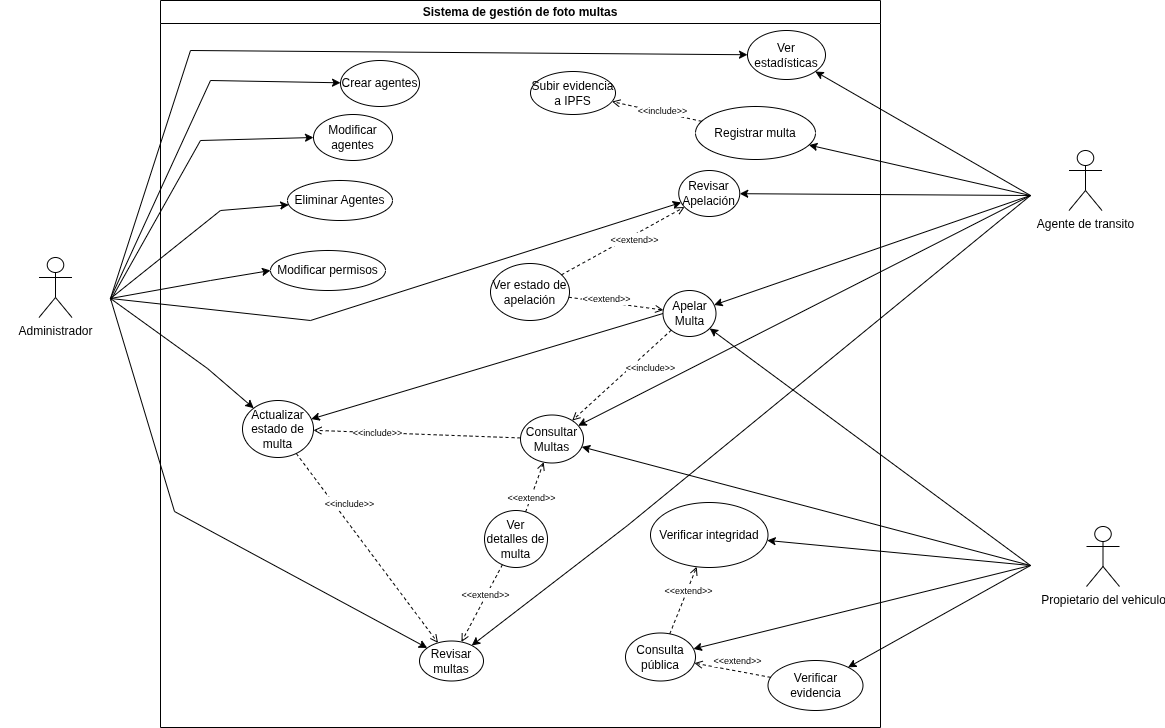
\includegraphics[width=0.8\textwidth]{Images/CasosUso.png}
    \caption{Diagrama de casos de uso del sistema de gestión de infracciones de tránsito.}
    \label{fig:casos_uso}
\end{figure}

 \subsection{ Diagrama de Despliegue }
\begin{figure}[htbp]
    \centering
    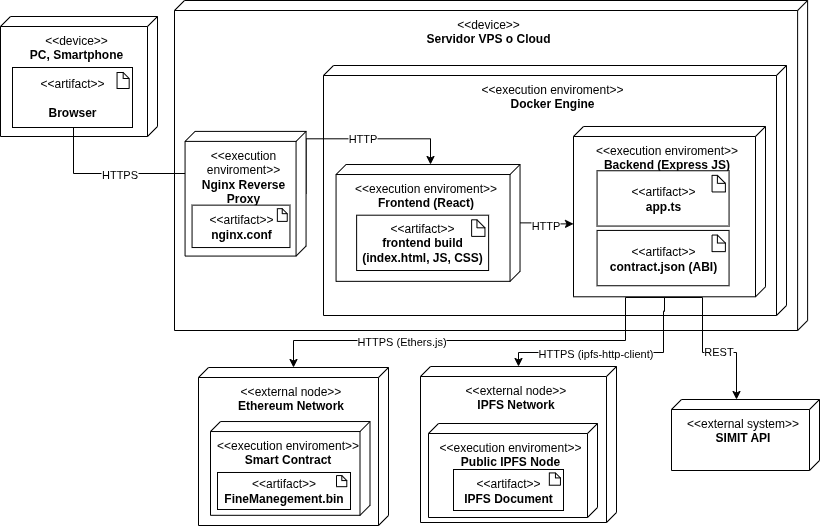
\includegraphics[width=0.8\textwidth]{Images/Despliegue.png}
    \caption{Diagrama de despliegue de la arquitectura del sistema.}
    \label{fig:diagrama_despliegue}
\end{figure}
En la Figura \ref{fig:diagrama_despliegue} se puede observar el diagrama de despliegue propuesto, donde cada nodo cuenta con la misma información, ya que esta se encontrará sincronizada. Asimismo, se conecta mediante servicios web a la base de datos de Apitude como herramienta de terceros para acceder a la información existente en el Registro Único Nacional de Tránsito (RUNT), de donde se obtendrán los datos de conductores, vehículos y el registro de infractores en Bogotá, así como el estado de las multas.

Hay que mencionar que existen dos soluciones para traer la información necesaria de estas entidades: la primera es una API llamada Apitude, de un tercero que provee la información del RUNT y del SIMIT; la segunda consiste en utilizar los datos que estas entidades públicas ya poseen en bases de datos tradicionales. 
 \subsection{ Diagrama de clases }
Hay que considerar que se manejarán dos capas de lógica: la primera enfocada en registrar los cambios en los estados de las multas a través de blockchain y la segunda capa encargada de la administración general de las multas (manipular los datos que no son visibles al público). 
 \begin{figure}[htbp]
    \centering
    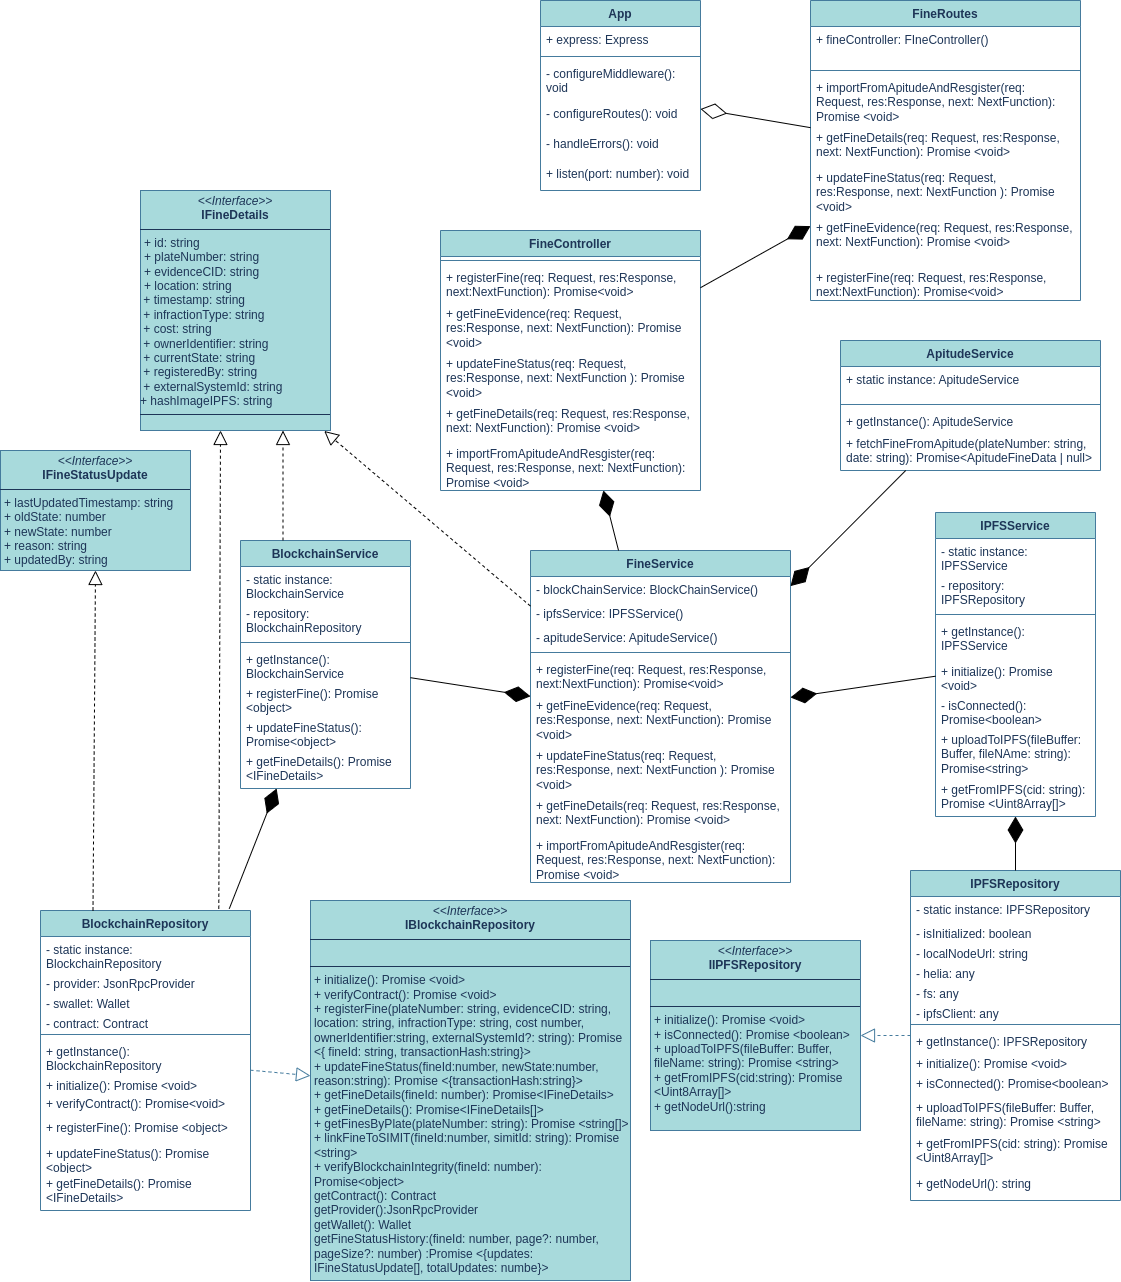
\includegraphics[width=0.8\textwidth]{Images/uml.png}
    \caption{Diagrama de clases del sistema de gestión de multas.}
    \label{fig:diagrama_clases}
\end{figure}
En la Figura \ref{fig:diagrama_clases} se hace un esquema de la primera capa lógica que se encarga de la administración general de las multas y los datos que maneja
 \begin{figure}[htbp]
    \centering
    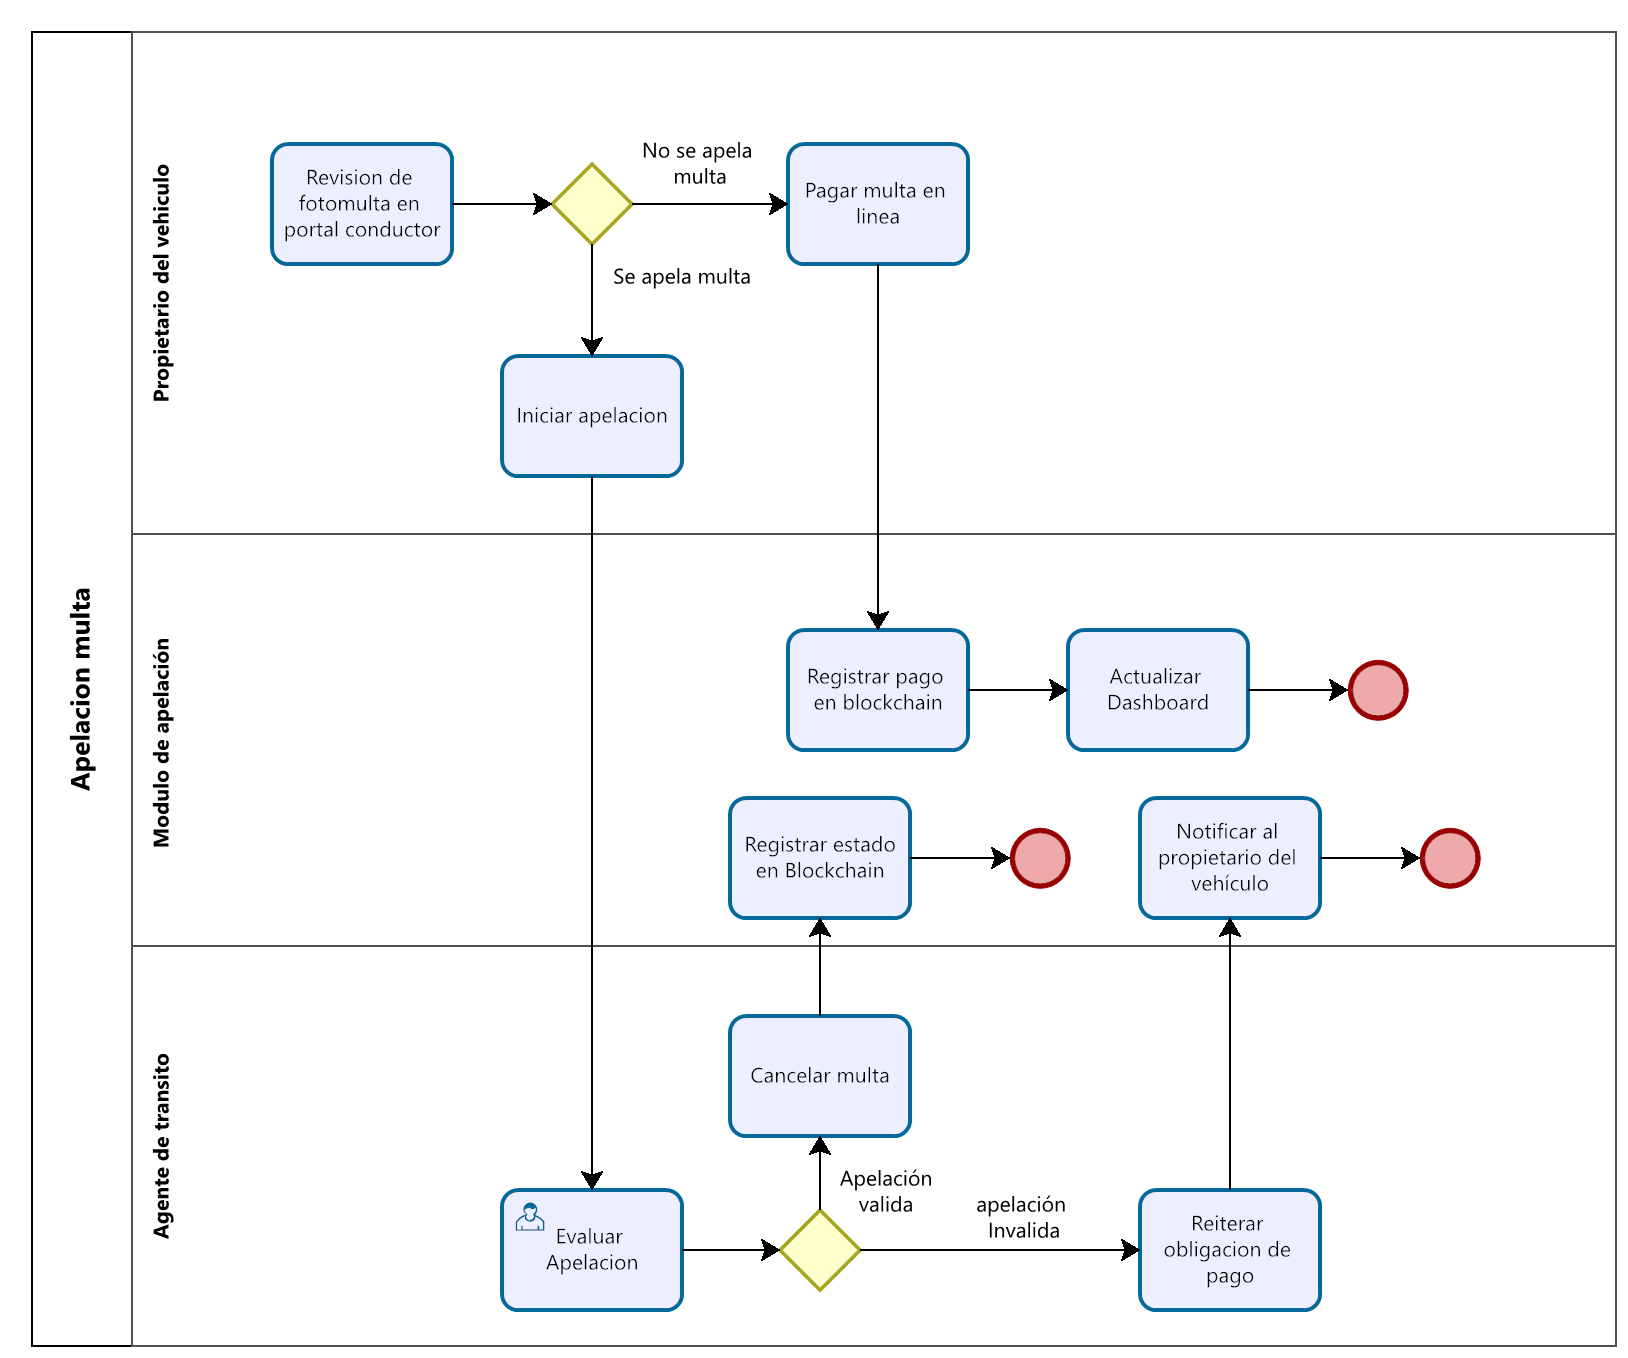
\includegraphics[width=0.8\textwidth]{Images/ActApelacion.png}
    \caption{Diagrama de actividades para el proceso de apelación de multa.}
    \label{fig:diagrama_apelacion}
\end{figure}
En la Figura \ref{fig:diagrama_apelacion} se hace mención en la segunda capa lógica la cual son los cambios generados en el registro de multas que registramos en la blockchain, que se traducen en los contratos realizados en solidity.
\subsection{ Diagrama de actividades }
 \begin{figure}[htbp]
    \centering
    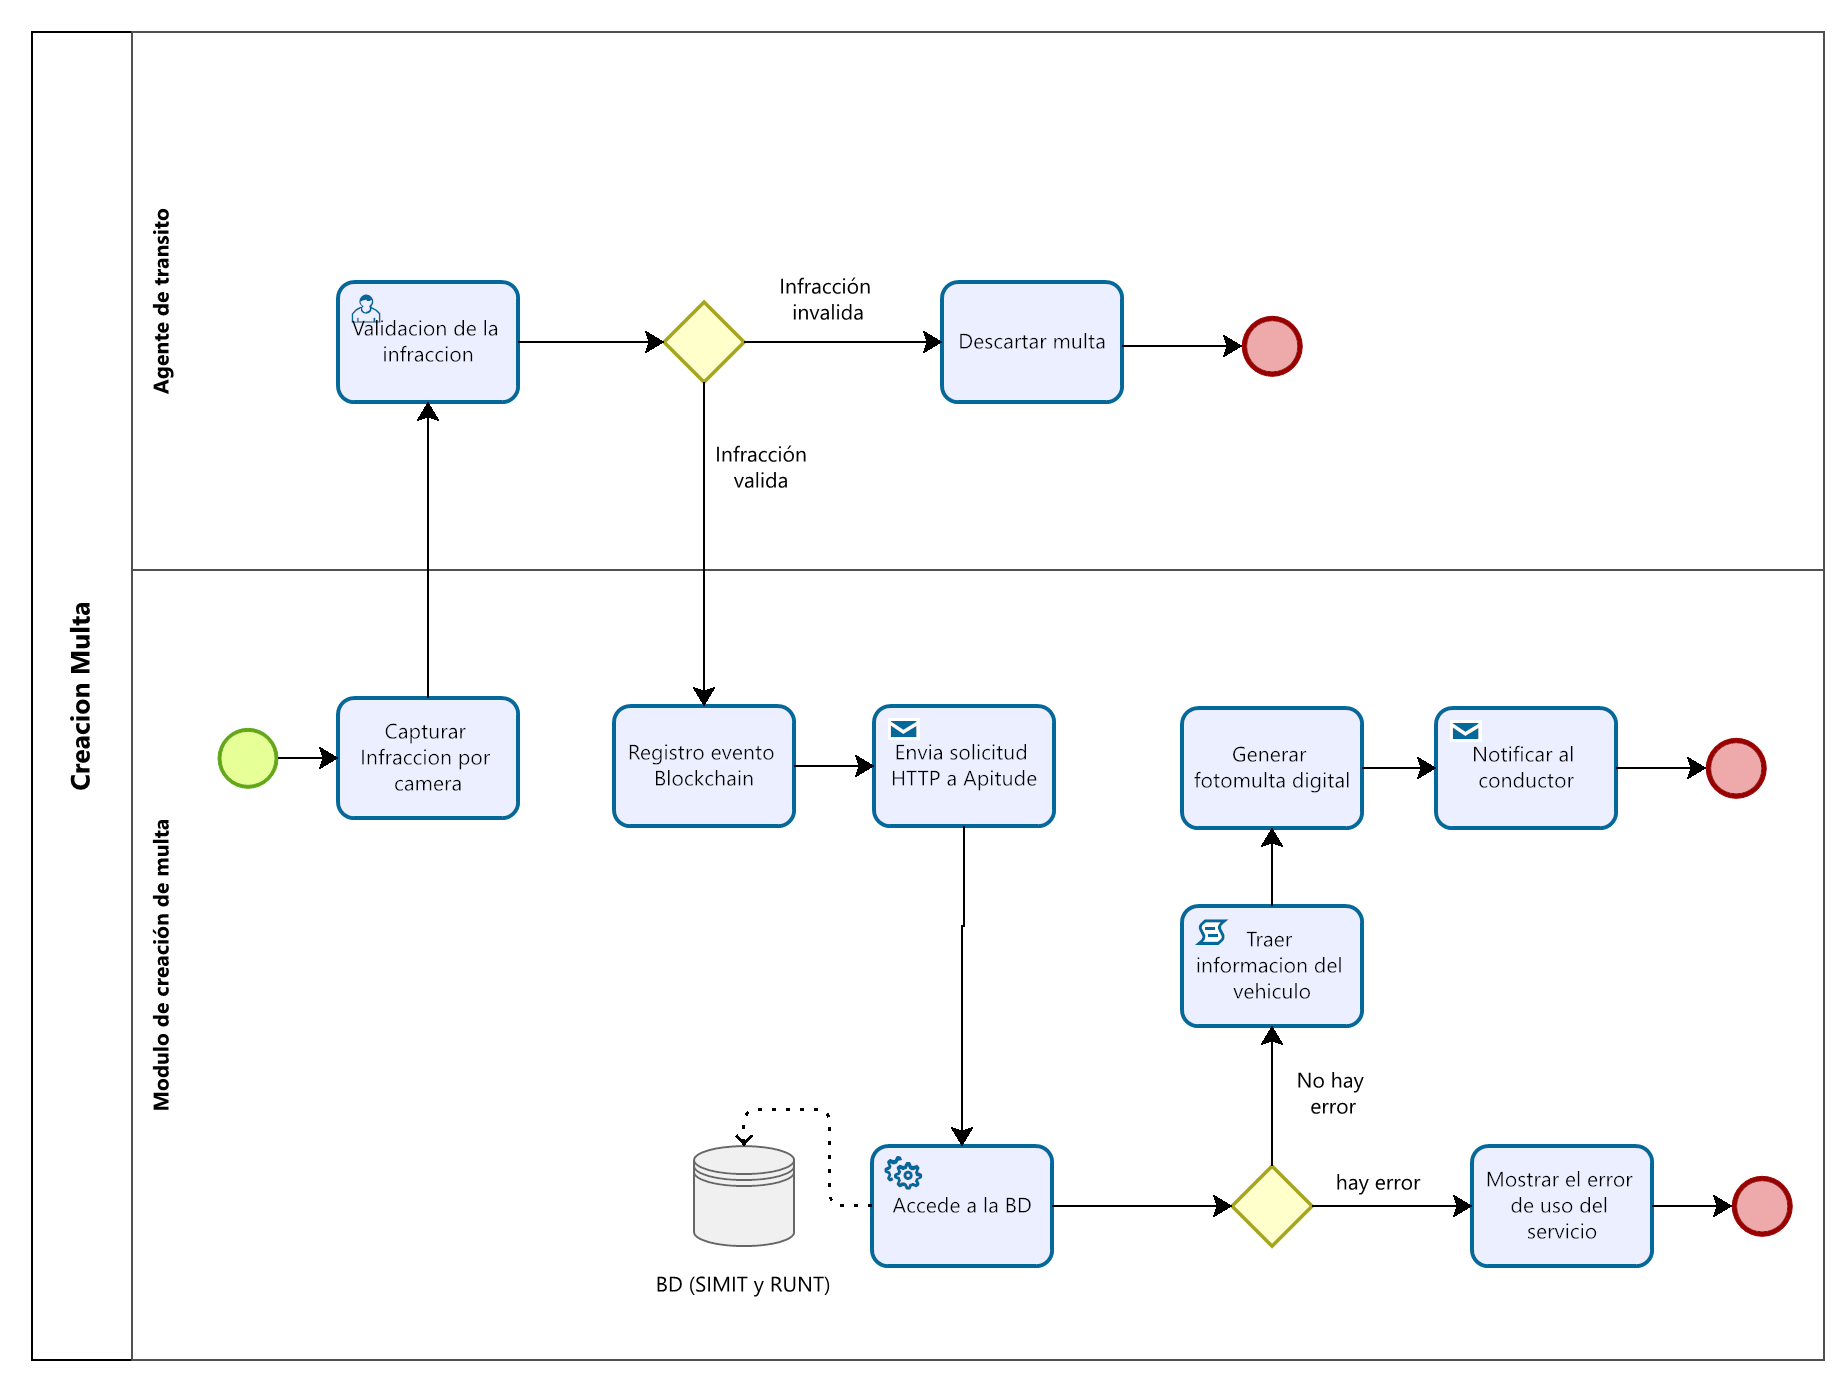
\includegraphics[width=0.8\textwidth]{Images/ActMulta.png}
    \caption{Diagrama de actividades para el proceso de creación de multa.}
    \label{fig:diagrama_creacion_multa}
\end{figure}
 \begin{figure}[htbp]
    \centering
    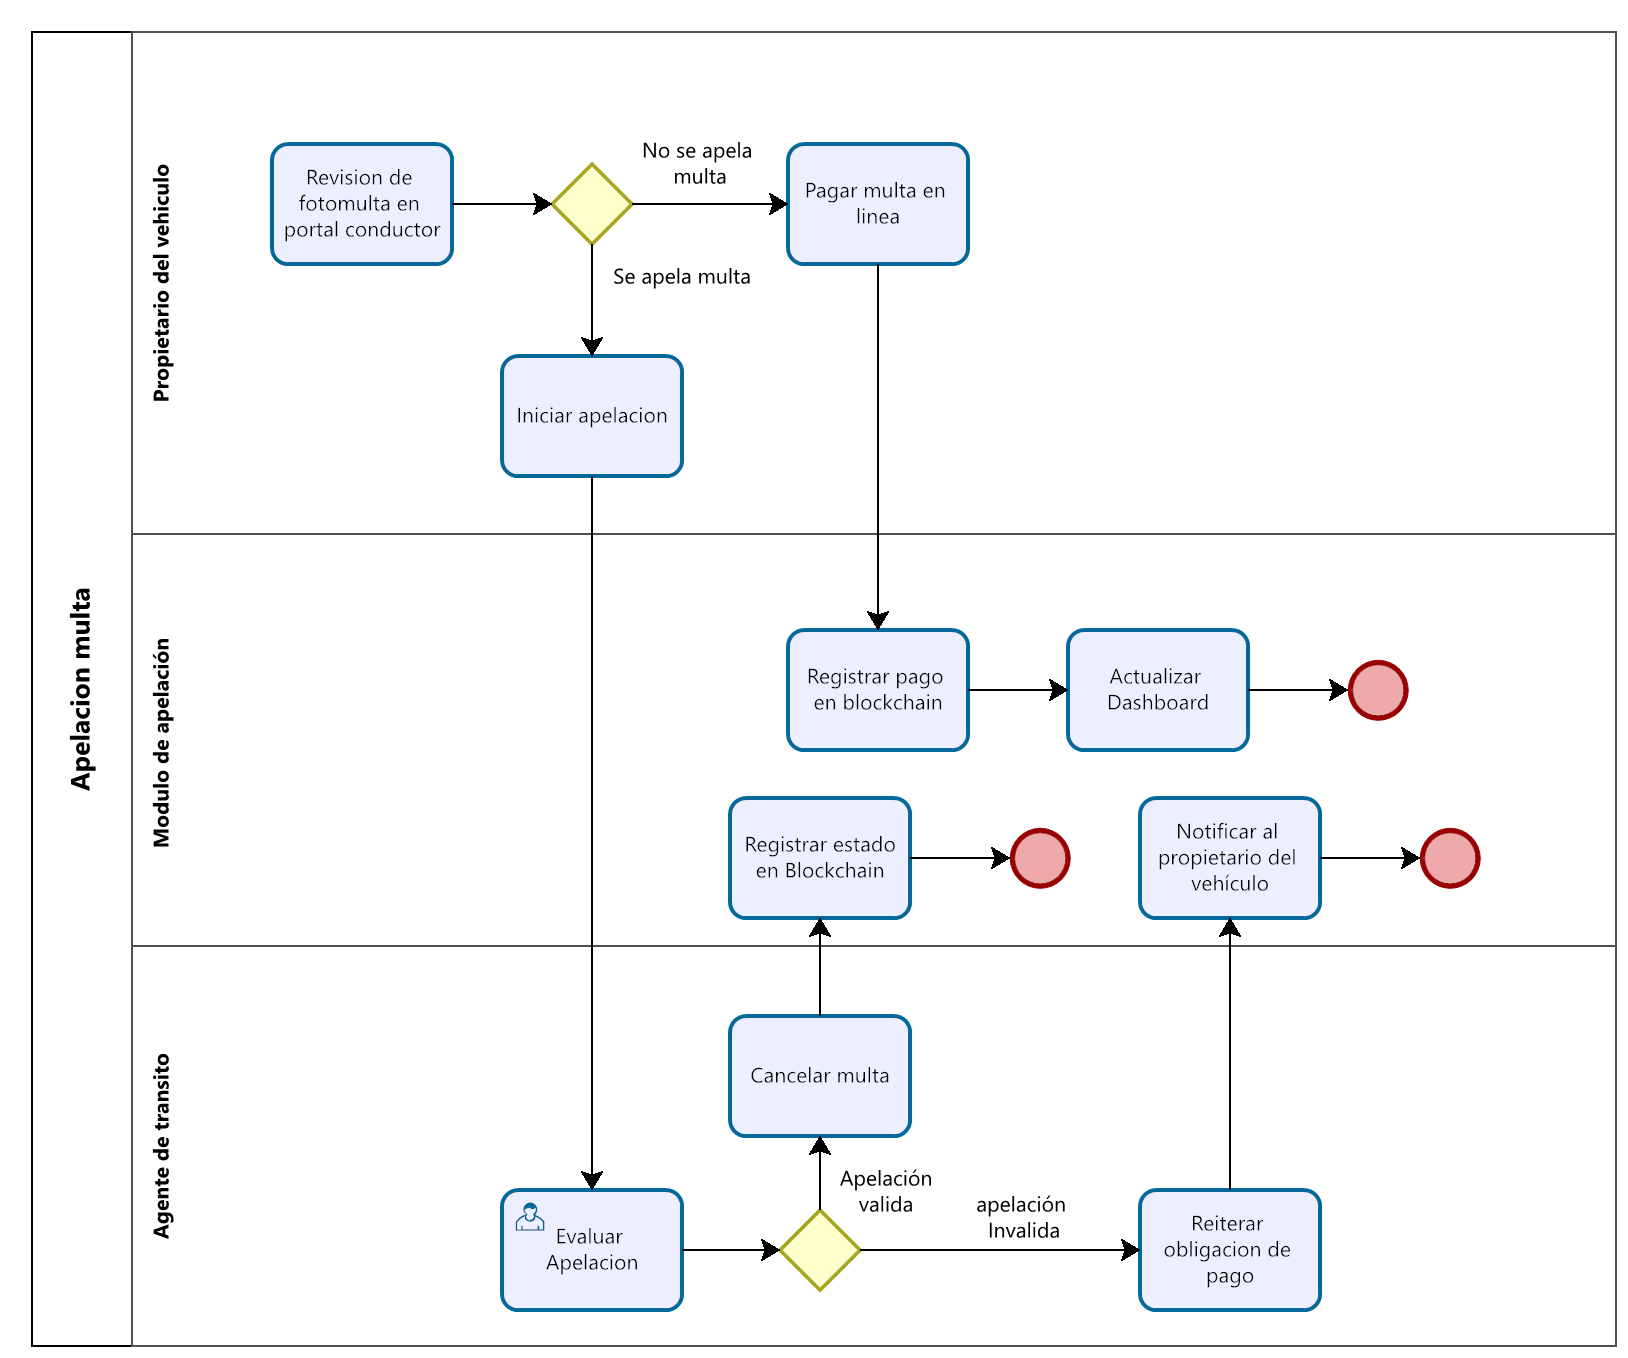
\includegraphics[width=0.8\textwidth]{Images/ActApelacion.png}
    \caption{Diagrama de actividades para el proceso de apelación de multa.}
    \label{fig:diagrama_apelacion_2}
\end{figure}

\subsection{Interfaz de Usuario}
\paragraph{Compartidas}
 \begin{figure}[htbp]
    \centering
    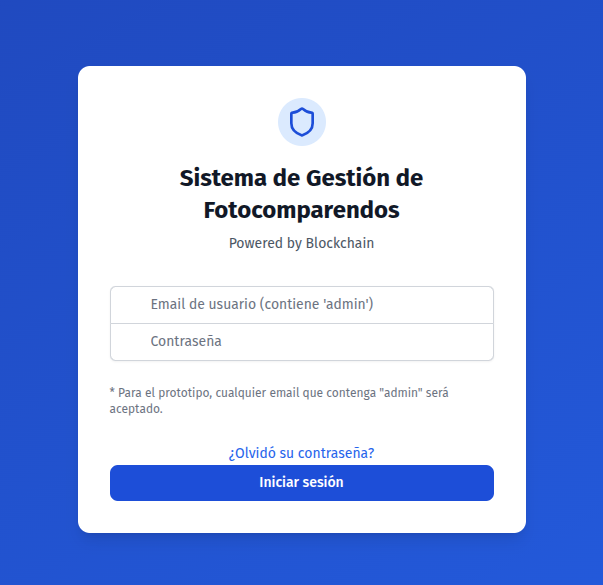
\includegraphics[width=0.8\textwidth]{Images/UI1.png}
    \caption{Pantalla de login del sistema.}
    \label{fig:login}
\end{figure}
+En la Figura~\ref{fig:login} se aprecia la pantalla de inicio de sesión, punto de entrada para todos los usuarios autorizados del sistema.

 \begin{figure}[htbp]
    \centering
    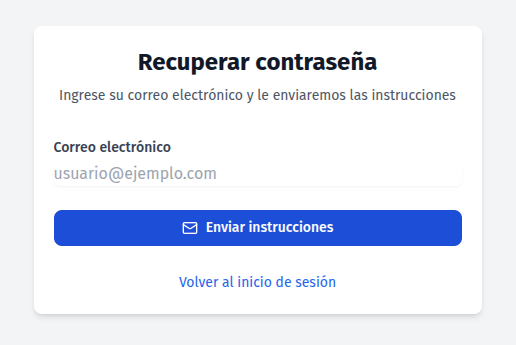
\includegraphics[width=0.8\textwidth]{Images/UI2.png}
    \caption{Pantalla de recuperación de contraseña.}
    \label{fig:recuperar_password}
\end{figure}
+La Figura~\ref{fig:recuperar_password} muestra el formulario para recuperar la contraseña, reforzando la experiencia de autoservicio y seguridad de la plataforma.
\paragraph{Vista Agente}
\begin{figure}[htbp]
    \centering
    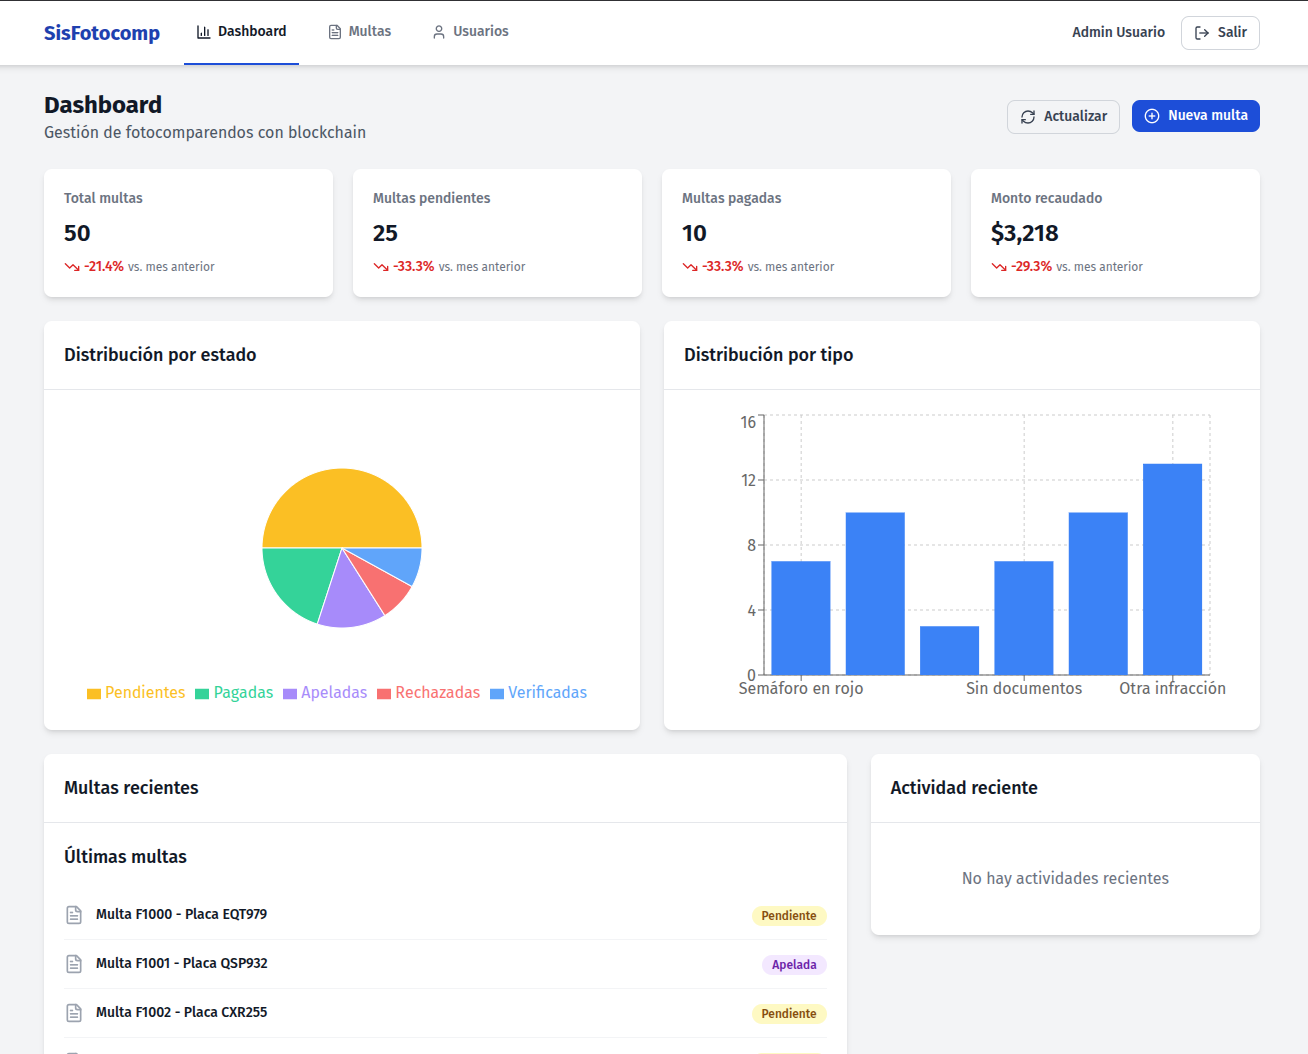
\includegraphics[width=0.8\textwidth]{Images/UI3.png}
    \caption{Dashboard del agente de tránsito.}
    \label{fig:dashboard_agente}
\end{figure}
+En la Figura~\ref{fig:dashboard_agente} se presenta el tablero principal que resume las métricas de gestión de multas para el agente de tránsito.
\begin{figure}[htbp]
    \centering
    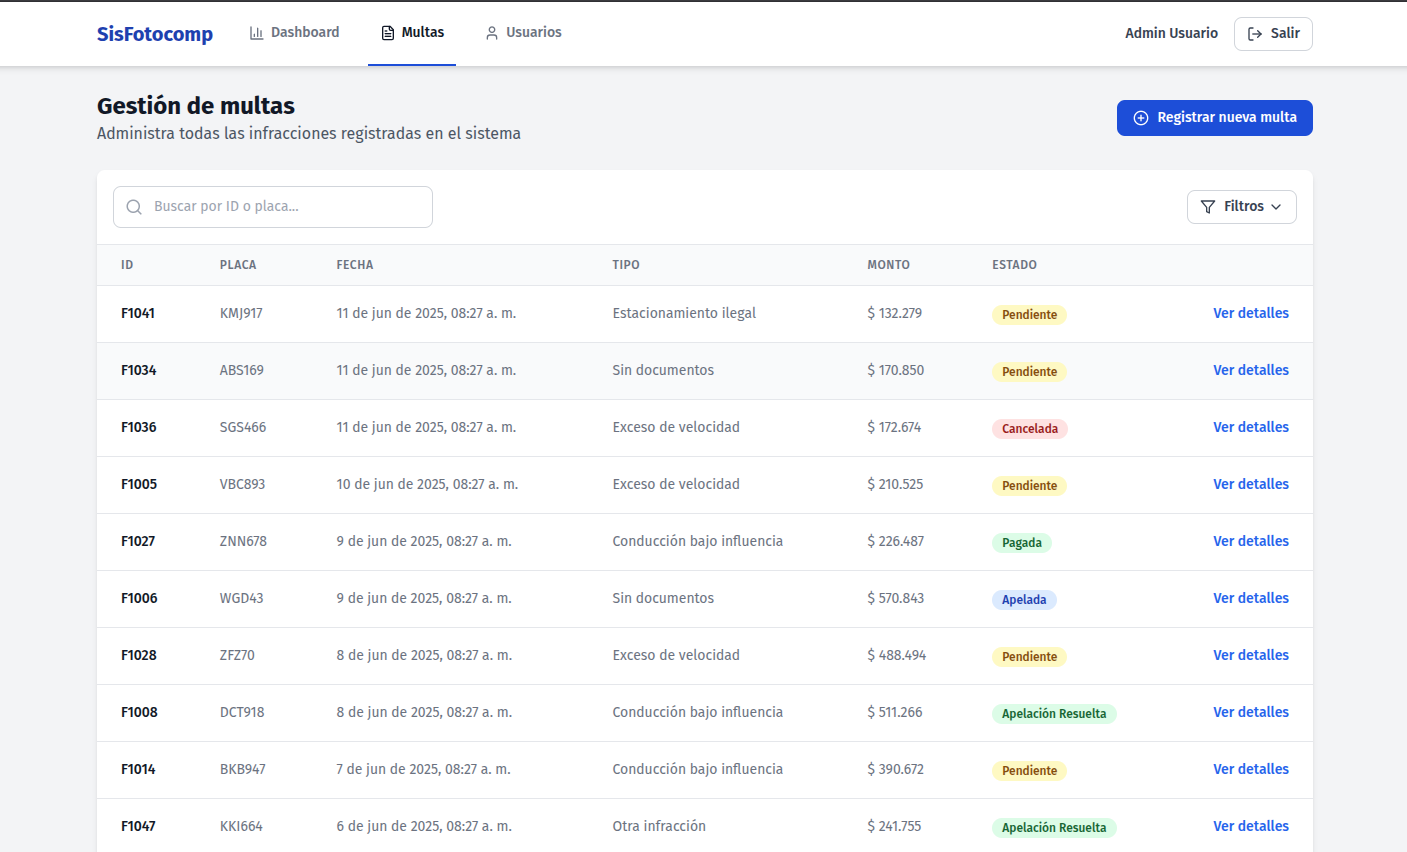
\includegraphics[width=0.8\textwidth]{Images/UI4.png}
    \caption{Pantalla de consulta del estado de multa.}
    \label{fig:consulta_estado_multa}
\end{figure}
+La Figura~\ref{fig:consulta_estado_multa} ilustra la consulta rápida del estado de una multa, facilitando el seguimiento por parte del agente.
\begin{figure}[htbp]
    \centering
    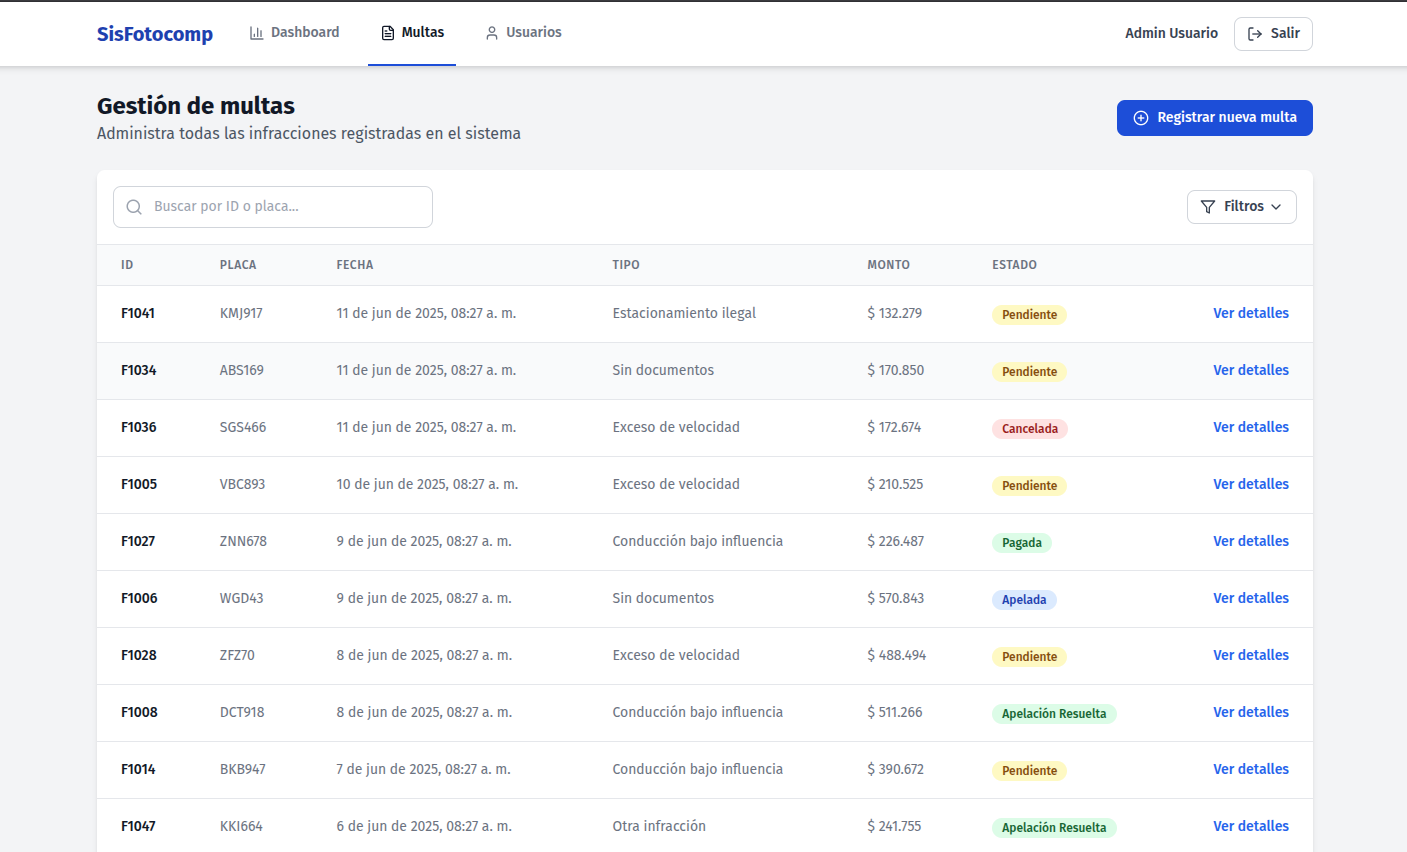
\includegraphics[width=0.8\textwidth]{Images/UI4.png}
    \caption{Pantalla de consulta de detalle de multa.}
    \label{fig:consulta_detalle_multa}
\end{figure}
+En la Figura~\ref{fig:consulta_detalle_multa} se muestra el detalle completo de una multa específica, incluida la evidencia asociada.
\paragraph{Vista Propietario de Vehiculo}
\begin{figure}[htbp]
    \centering
    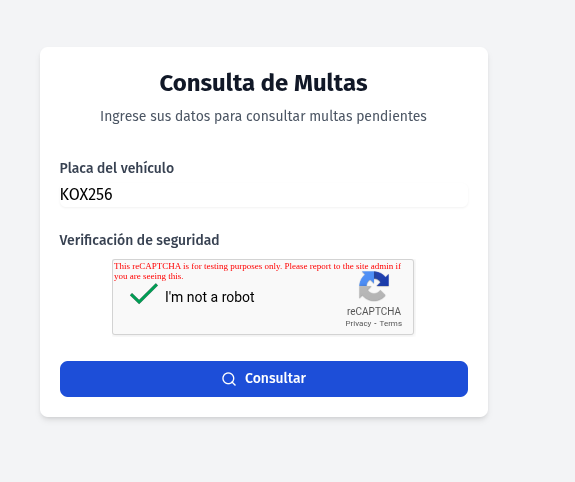
\includegraphics[width=0.8\textwidth]{Images/UI5.png}
    \caption{Pantalla de consulta de multas para propietarios de vehículos.}
    \label{fig:consulta_multas_propietario}
\end{figure}
+Por último, la Figura~\ref{fig:consulta_multas_propietario} exhibe la vista que permite al propietario del vehículo revisar todas sus multas pendientes o en proceso. 
\section{Costos del Proyecto}
\paragraph{Resumen de costos}

\begin{figure}[htbp]
    \begin{flushleft}
        \textbf{Figura 2}\\[2em]
        \textit{Resumen de costos del proyecto}
    \end{flushleft}
    \vspace{1em}
    \addcontentsline{lof}{figure}{Figura 2. Resumen de costos del proyecto}
    \centering
    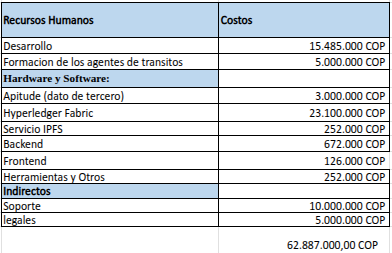
\includegraphics[width=\textwidth]{Images/costos1.png}
    \vspace{2em}
    \begin{flushleft}
        \textit{Nota.} Elaboración propia.
    \end{flushleft}
    \refstepcounter{figure}\label{fig:costos1}
\end{figure}

Este proyecto involucra el desarrollo e implementación de un sistema de software complejo que utiliza tecnologías modernas como blockchain (Hyperledger Fabric) e IPFS, junto con componentes web tradicionales (React, Express.js). Los costos se han estimado cuidadosamente considerando el esfuerzo de desarrollo, la infraestructura necesaria, la capacitación y otros gastos indirectos. 

En la Figura~\ref{fig:costos1} se presenta un resumen de los costos del proyecto. El costo total estimado asciende a 62.887.000,00 COP. Este monto se desglosa en varias categorías principales que detallaremos a continuación, basándonos en una estimación ascendente del esfuerzo y una proyección de los costos de infraestructura y servicios. 

\paragraph{Costos de Software y Hardware}

\begin{figure}[htbp]
    \begin{flushleft}
        \textbf{Figura 3}\\[2em]
        \textit{Estimación de costos mensuales de infraestructura}
    \end{flushleft}
    \vspace{1em}
    \addcontentsline{lof}{figure}{Figura 3. Estimación de costos mensuales de infraestructura}
    \centering
    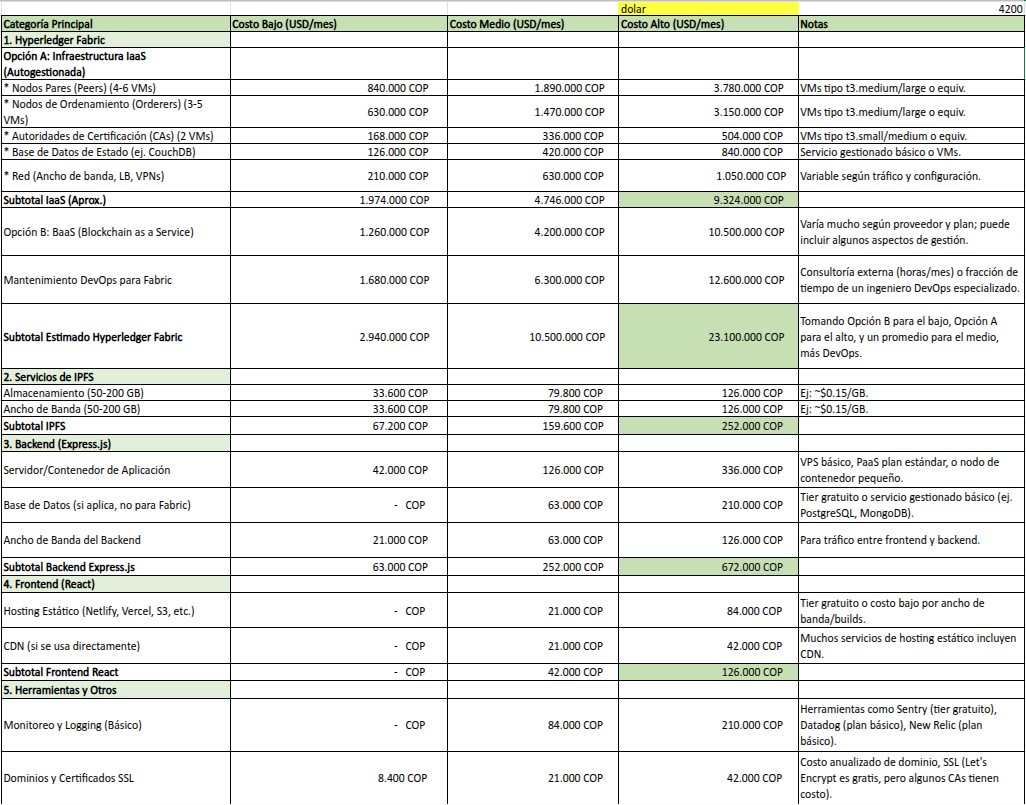
\includegraphics[width=\textwidth]{Images/costos2.png}
    \vspace{2em}
    \begin{flushleft}
        \textit{Nota.} Elaboración propia.
    \end{flushleft}
    \refstepcounter{figure}\label{fig:costos2}
\end{figure}

La Figura~\ref{fig:costos2} proyecta los costos mensuales recurrentes asociados con la infraestructura necesaria para desplegar y operar la aplicación. Ofrece tres escenarios (Bajo, Medio, Alto) para cada componente, reflejando diferentes niveles de capacidad, rendimiento o robustez. Los valores en esta tabla están originalmente en dólares (USD) y se han convertido a pesos colombianos (COP) utilizando una tasa de cambio de 4.200 COP/USD (según la celda indicada). Se ha seleccionado el escenario "Costo Alto (USD/mes)" para alimentar la tabla de "Resumen de Costos". 

\paragraph{Categorías Principales y Subcomponentes (basado en el escenario "Alto" seleccionado): }

\begin{enumerate}
\item \textbf{Hyperledger Fabric:} Es el costo más significativo, reflejando la complejidad de desplegar y mantener una red blockchain permisionada. 

\begin{itemize}
\item \textbf{Infraestructura IaaS (Autogestionada) o BaaS:} Incluye servidores para nodos pares, nodos de ordenamiento, autoridades de certificación, bases de datos de estado y costos de red. El escenario alto seleccionado suma 9.324.000 COP. 

\item \textbf{Mantenimiento DevOps para Fabric:} Un costo crucial para la operación, monitoreo y actualización de la red Fabric, estimado en 12.600.000 COP. 

\item\textbf{Subtotal Estimado Hyperledger Fabric:} 23.100.000 COP (Nota: parece haber una pequeña diferencia entre la suma de los componentes IaaS y DevOps, y el subtotal. El subtotal de 23.100.000 COP es el que se traslada al resumen). 
\end{itemize}
\item \textbf{Servicios de IPFS:} Costos asociados al almacenamiento y ancho de banda para el 		sistema de archivos descentralizado, estimados en 252.000 COP. 

\item \textbf{Backend (Express.js):} Costos del servidor de aplicación, base de datos (si aplica fuera de Fabric) y ancho de banda para la API, sumando 672.000 COP. 

\item \textbf{Frontend (React):} Costos de hosting estático y CDN para la interfaz de usuario, estimados en 126.000 COP. 

\item \textbf{Herramientas y Otros:} Incluye monitoreo, logging, dominios y certificados SSL, con un costo de 252.000 COP. 
\end{enumerate}
 

\textbf{GRAN TOTAL ESTIMADO MENSUAL (Escenario Alto):} El costo mensual recurrente total para la infraestructura y servicios, en el escenario alto, es de 24.402.000 COP. Nota: Este es el costo mensual. En la tabla de resumen de costos, algunos de estos se presentan como si fueran un costo único o para un periodo específico, lo cual habría que aclarar (ej. si el costo de Hyperledger Fabric de 23.100.000 COP es para el primer mes, o para un periodo de setup y algunos meses de operación). Si es mensual, el total del proyecto se dispararía si es para muchos meses. 

\medskip
\textit{Nota del equipo de proyecto:} Este capítulo permanecerá provisionalmente para fines de trazabilidad. Se contempla su eliminación o reemplazo por un anexo financiero detallado en versiones futuras, una vez se definan los modelos de despliegue y financiación definitivos.

\paragraph{Costo de Desarrollo }
\begin{figure}[htbp]
    \begin{flushleft}
        \textbf{Figura 4}\\[2em]
        \textit{Estimación de costos de desarrollo del proyecto}
    \end{flushleft}
    \vspace{1em}
    \addcontentsline{lof}{figure}{Figura 4. Estimación de costos de desarrollo del proyecto}
    \centering
    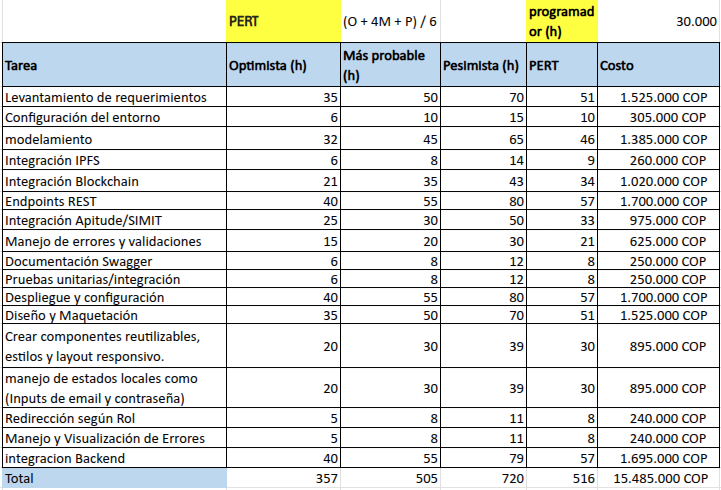
\includegraphics[width=\textwidth]{Images/costos3.png}
    \vspace{2em}
    \begin{flushleft}
        \textit{Nota.} Elaboración propia.
    \end{flushleft}
    \refstepcounter{figure}\label{fig:costos3}
\end{figure}

La Figura~\ref{fig:costos3} detalla el esfuerzo estimado para cada tarea específica del desarrollo del software. Utiliza la técnica PERT (Program Evaluation and Review Technique) para calcular un tiempo ponderado (columna "PERT (h)") basándose en estimaciones optimistas, más probables y pesimistas. Este esfuerzo en horas se traduce luego en un costo, asumiendo una tarifa por hora de programador de 30.000 COP (según la celda "programador (h)"). 
\paragraph{Columnas Clave: }
\begin{itemize}
\item \textbf{Tarea:} Describe las actividades individuales de desarrollo, desde el levantamiento de requerimientos hasta el despliegue y diseño. 

\item \textbf{Optimista (h), Más probable (h), Pesimista (h):} Son las tres estimaciones de tiempo para cada tarea, fundamentales para la técnica PERT. 

\item \textbf{PERT (h): }Es el tiempo estimado ponderado calculado con la fórmula (Optimista + 4 * Más probable + Pesimista) / 6. Este valor representa una estimación más realista del tiempo que tomará cada tarea, considerando la incertidumbre. 

\item \textbf{Costo}: Es el resultado de multiplicar las horas PERT por la tarifa horaria del programador (30.000 COP). 
\end{itemize}
 

\paragraph{Total de Desarrollo:} El costo total de desarrollo de software asciende a 15.485.000 COP, correspondiente a un esfuerzo total estimado de 516 horas PERT. Esto cubre todas las fases del ciclo de vida del desarrollo, incluyendo la integración con IPFS, Blockchain, el desarrollo de Endpoints REST, pruebas, y la creación de la interfaz de usuario. 
\section{Plan de pruebas}

\subsection{Introducción y propósito}
El propósito de este plan es guiar la evaluación de la efectividad y viabilidad del prototipo desarrollado para la gestión de fotocomparendos utilizando Hyperledger Fabric e IPFS. Se busca validar que el prototipo cumple con los requisitos clave de inmutabilidad, transparencia, seguridad, y medir su rendimiento básico, comparándolo con las limitaciones identificadas en el sistema tradicional de Bogotá.

\subsection{Alcance de las pruebas}
\begin{itemize}
    \item Proceso completo de registro de un fotocomparendo: captura simulada, carga de evidencia a IPFS, registro de metadatos y hash IPFS en el ledger.
    \item Consulta y verificación de fotocomparendos registrados.
    \item Verificación de la inmutabilidad de los registros en el ledger y de la evidencia en IPFS.
    \item Consistencia de los datos entre la UI, el ledger y IPFS.
    \item Rendimiento básico de operaciones clave (registro, consulta).
    \item Actualización del estado de la multa (ej. "Pagada", "Apelada").
\end{itemize}

\subsection{Fuera de alcance}
\begin{itemize}
    \item Pruebas de estrés o carga exhaustivas.
    \item Pruebas de penetración de seguridad avanzadas.
    \item Integración completa con sistemas externos reales (RUNT, SIMIT) más allá de APIs simuladas o de prueba.
    \item Pruebas de usabilidad exhaustivas con usuarios finales.
    \item Funcionalidad de pago automatizado con billetera digital.
\end{itemize}

\subsection{Entorno de pruebas (simulación controlada)}
\paragraph{Hardware}
\begin{itemize}
    \item Servidor(es) para nodos Hyperledger Fabric (pueden ser VMs o contenedores Docker). 
    \item Servidor(es) para nodo(s) IPFS (pueden ser VMs o contenedores Docker). 
    \item Máquina para ejecutar la aplicación backend (Node.js/Express según). 
    \item Máquinas cliente para acceder a la interfaz web (simulando Agente de Movilidad y Ciudadano).
\end{itemize}
\paragraph{Software}
\begin{itemize}
    \item Hyperledger Fabric (versión específica). 
    \item IPFS (Kubo/Helia, versión específica).
    \item Base de datos (si la aplicación backend la usa adicionalmente). 
    \item Aplicación backend (Node.js, Express, etc.).
        \item Aplicación frontend (navegador web). 
    \item Herramientas de monitoreo y logging.
\end{itemize}
\paragraph{Datos de prueba}
\begin{itemize}
    \item Conjunto de imágenes de evidencia (JPG, PNG) de diferentes tamaños. 
    \item Datos de fotocomparendos ficticios (placas, fechas, ubicaciones, tipos de infracción). 
    \item Datos de usuarios simulados (Agentes de Movilidad, Administradores, Ciudadanos).
\end{itemize}

\subsection{Tipos de pruebas y casos de prueba detallados}

% Tabla de casos de prueba funcionales
\paragraph{Pruebas Funcionales}
\begin{table}[htbp]
    \centering
    \footnotesize
    \caption{Casos de Prueba Funcionales}
    \label{tab:casos_funcionales}

    \begin{tabular}{|
        >{\raggedright\arraybackslash}p{0.07\textwidth}|
        >{\raggedright\arraybackslash}p{0.20\textwidth}|
        >{\raggedright\arraybackslash}p{0.40\textwidth}|
        >{\raggedright\arraybackslash}p{0.20\textwidth}|}
        \hline
        \textbf{ID} & \textbf{Descripción} & \textbf{Pasos de Ejecución} & \textbf{Datos de Entrada} \\
        \hline
        % Fila 1
        \textbf{FT-001} & 
        Registro exitoso de fotocomparendo & 
        1. Login en SisFotocomp. \newline 
        2. Ir a "Registrar nueva multa". \newline 
        3. Ingresar datos (placa, fecha, tipo). \newline 
        4. Adjuntar imagen. \newline 
        5. Enviar. & 
        Placa: XYZ789, Fecha: [Hoy], Tipo: Exceso Velocidad, Imagen: evidencia01.jpg \\
        \hline
        % Fila 2
        \textbf{FT-002} & 
        Consulta y verificación (Agente/Admin) & 
        1. Login como Agente/Admin. \newline 
        2. Ir a "Gestión de multas". \newline 
        3. Buscar multa FT-001 por ID o placa. \newline 
        4. Ver detalles. \newline 
        5. Verificar información e imagen IPFS. & 
        ID/Placa de la multa FT-001. \\
        \hline
        % Fila 3
        \textbf{FT-003} & 
        Consulta ciudadana & 
        1. Acceder a "Consulta de Multas". \newline 
        2. Ingresar documento, número y placa. \newline 
        3. Ingresar CAPTCHA. \newline 
        4. Consultar. & 
        Datos del propietario/vehículo de FT-001. \\
        \hline
        % Fila 4
        \textbf{FT-004} & 
        Registro con datos incompletos & 
        1. Intentar registrar multa sin placa o sin imagen. & 
        Placa: Vacía, Imagen: No adjuntada. \\
        \hline
        % Fila 5
        \textbf{FT-005} & 
        Actualización de estado & 
        1. Seleccionar multa FT-001. \newline 
        2. Cambiar estado (ej. "Apelada", "Pagada"). \newline 
        3. Guardar. & 
        Multa FT-001, Nuevo estado: "Apelada". \\
        \hline
        % Fila 6
        \textbf{FT-006} & 
        Consistencia Ledger-IPFS & 
        1. Registrar multa (similar a FT-001). \newline 
        2. Anotar CID de IPFS y metadatos. \newline 
        3. Recuperar transacción del ledger. \newline 
        4. Recuperar imagen de IPFS. & 
        Nueva multa, nueva imagen. \\
        \hline
    \end{tabular}
\end{table} 

\noindent En la Tabla~\ref{tab:casos_prueba_funcionales} se enumeran los casos de prueba funcionales definidos para verificar el comportamiento básico del sistema, desde el registro de un fotocomparendo hasta la validación de su integridad y actualización de estado. Cada caso detalla las precondiciones, las acciones a ejecutar y el resultado esperado, sirviendo como guía para las pruebas manuales y automatizadas.

\subsection{Pruebas de inmutabilidad}

% Tabla de casos de prueba de inmutabilidad
\begin{table}[htbp]
    \begin{flushleft}
        \textbf{Tabla 3}\\[1em]
        \textit{Casos de prueba de inmutabilidad para validar resistencia a modificaciones}
    \end{flushleft}
    \vspace{1em}
    \addcontentsline{lot}{table}{Tabla 3. Casos de prueba de inmutabilidad para validar resistencia a modificaciones}
    \centering
    \begin{tabular}{p{2cm} p{6cm} p{4cm}}
        \toprule
        \textbf{ID} & \textbf{Caso de Prueba} & \textbf{Objetivo} \\
        \midrule
        IM-001 & Intento de modificación directa en ledger & Verificar resistencia a cambios no autorizados \\
        IM-002 & Alteración de imagen en IPFS & Validar detección de modificaciones en evidencia \\
        IM-003 & Verificación de trazabilidad & Comprobar integridad del historial transaccional \\
        IM-004 & Validación de consenso & Evaluar mecanismos de protección distribuida \\
        \bottomrule
    \end{tabular}
    \vspace{1em}
    \begin{flushleft}
        \textit{Nota.} Elaboración propia.
    \end{flushleft}
    \refstepcounter{table}\label{tab:casos_prueba_inmutabilidad}
\end{table}

% Tabla de resultados de pruebas de inmutabilidad
\begin{table}[htbp]
    \begin{flushleft}
        \textbf{Tabla 4}\\[1em]
        \textit{Resultados de pruebas de inmutabilidad del sistema}
    \end{flushleft}
    \vspace{1em}
    \addcontentsline{lot}{table}{Tabla 4. Resultados de pruebas de inmutabilidad del sistema}
    \centering
    \begin{tabular}{p{3cm} p{4cm} p{3cm} p{3cm}}
        \toprule
        \textbf{Caso de Prueba} & \textbf{Descripción} & \textbf{Resultado Esperado} & \textbf{Resultado Real} \\
        \midrule
        IM-001 & Modificación directa en ledger & Transacción rechazada & Rechazada correctamente \\
        IM-002 & Cambio de imagen en IPFS & CID diferente generado & CID distinto detectado \\
        IM-003 & Verificación de trazabilidad & Historial inmutable & Historial preservado \\
        IM-004 & Validación de consenso & Consenso mantenido & Consenso validado \\
        \bottomrule
    \end{tabular}
    \vspace{1em}
    \begin{flushleft}
        \textit{Nota.} Elaboración propia.
    \end{flushleft}
    \refstepcounter{table}\label{tab:resultados_inmutabilidad}
\end{table} 

\noindent La Tabla~\ref{tab:casos_prueba_inmutabilidad} detalla los escenarios diseñados para poner a prueba la inmutabilidad del sistema ante intentos de modificación no autorizada, mientras que la Tabla~\ref{tab:resultados_inmutabilidad} resume los resultados obtenidos en dichas pruebas, evidenciando la correcta detección y rechazo de cambios indebidos.

\subsection{Pruebas de rendimiento básico}
Se midió el tiempo requerido para ejecutar operaciones clave en condiciones simuladas de uso real:

\begin{table}[htbp]
    \centering
    \caption{Tiempos promedio de operaciones en el entorno de prueba}
    \begin{tabular}{|p{4cm}|p{3cm}|}
        \hline
        \textbf{Operación} & \textbf{Tiempo Promedio (s)} \\
        \hline
        Registro completo (Blockchain + IPFS) & 1.60 \\
        \hline
        Consulta de evidencia desde IPFS & 0.80 \\
        \hline
        Validación de integridad & 0.90 \\
        \hline
    \end{tabular}
    \vspace{1em}
    \begin{flushleft}
        \textit{Nota.} Elaboración propia.
    \end{flushleft}
\end{table}


\subsection{Casos de prueba de inmutabilidad y verificabilidad}

\begin{center}
\begin{tabular}{|p{4cm}|p{3cm}|p{3cm}|p{3cm}|}
    \hline
    \textbf{Caso de Prueba} & \textbf{Objetivo} & \textbf{Resultado Esperado} & \textbf{Resultado Real} \\
    \hline
    Registro de comparendo con CID válido & Verificar registro inicial & Registro exitoso e inmutable & Registro correcto \\
    \hline
    Intento de modificación de metadatos post-registro & Comprobar resistencia a cambios internos & Transacción rechazada o inconsistente detectada & Inconsistencia detectada \\
    \hline
    Carga de imagen modificada (pixel cambiado) & Validar detección de alteraciones en imagen & CID diferente, evidencia no válida & CID distinto generado \\
    \hline
    Consulta ciudadana por endpoint \texttt{/integrity} & Evaluar mecanismo de verificación independiente & Imagen original y metadatos coinciden & Evidencia verificada \\
    \hline
\end{tabular}

\vspace{1em}
\noindent\textbf{Cuadro 3}\\[2em]
\textit{Casos de prueba de inmutabilidad y verificabilidad del sistema}
\end{center} 

\subsection{Estrategia de pruebas del frontend}

\paragraph{Introducción}
El frontend de la aplicación de gestión de multas implementa una estrategia integral de pruebas que abarca tanto pruebas unitarias como de integración, utilizando las mejores prácticas de testing en React con TypeScript. Esta estrategia garantiza la calidad del código, facilita el mantenimiento y reduce la introducción de errores durante el desarrollo.

\subsubsection{Herramientas y tecnologías}
\begin{itemize}
    \item \textbf{Jest}: Framework principal de testing con soporte para TypeScript.
    \item \textbf{React Testing Library}: Biblioteca para testing de componentes React con enfoque en comportamiento del usuario.
    \item \textbf{@testing-library/jest-dom}: Matchers adicionales para Jest.
    \item \textbf{@testing-library/user-event}: Simulación de eventos de usuario.
    \item \textbf{jsdom}: Entorno DOM para pruebas en Node.js.
\end{itemize}

\subsubsection{Pruebas unitarias}

\subsubsection{Pruebas de integración}

\section{Resultados de las Pruebas de Inmutabilidad y Verificabilidad del Prototipo}

Con el fin de validar los principios fundamentales sobre los que se sustenta el presente prototipo —particularmente la \textbf{inmutabilidad}, \textbf{integridad de evidencia} y \textbf{verificabilidad independiente}— se diseñó y ejecutó un plan de pruebas en entorno simulado controlado, alineado con los objetivos del proyecto y los estándares técnicos de la literatura especializada. Las pruebas se enfocaron en evaluar el comportamiento del sistema frente a intentos de modificación, errores de integridad y recuperación de evidencia a través de mecanismos descentralizados.

\subsection{Pruebas de Inmutabilidad en Blockchain}

Se registraron comparendos en la red \textit{Ethereum local (Hardhat)}, incluyendo el hash IPFS (CID) de la evidencia fotográfica y los metadatos del evento. Luego, se intentó simular una alteración directa sobre el estado del ledger.

\textbf{Resultado:} El sistema rechazó cualquier intento de modificación, manteniendo el hash original y evidenciando que la estructura de bloques y el mecanismo de consenso impiden alteraciones sin detección. Esto confirma que el sistema ofrece \textbf{inmutabilidad verificable} en los registros sancionatorios.

\subsection{Verificación de Integridad con IPFS}

Se almacenaron imágenes en IPFS y se compararon los CIDs obtenidos con nuevos hashes locales generados al momento de la consulta.

\textbf{Resultado:} Se comprobó que el CID siempre coincide con el contenido original. Cualquier cambio, incluso mínimo, genera un CID diferente, por lo que el sistema detecta automáticamente cualquier intento de manipulación. Esto demuestra que la evidencia permanece \textbf{íntegra y detectable ante alteraciones}.

\subsection{Verificabilidad Transparente del Registro}

Se implementó un mecanismo de consulta pública (\texttt{/api/fines/:fineId/integrity}) que permite a cualquier parte autorizada extraer el CID desde la Blockchain y verificar que la evidencia recuperada desde IPFS corresponde al evento sancionado.

\textbf{Resultado:} La verificación se ejecuta sin intervención humana, desde fuentes independientes, replicando los principios de \textbf{transparencia, auditabilidad y confianza descentralizada}.

\subsection{Casos de Prueba Funcionales}

% Tablas de resultados de pruebas

\subsection{Casos de Prueba Funcionales}

\begin{table}[htbp]
    \begin{flushleft}
        \textbf{Tabla 5}\\[2em]
        \textit{Resultados de pruebas funcionales del sistema}
    \end{flushleft}
    \vspace{1em}
    \addcontentsline{lot}{table}{Tabla 5. Resultados de pruebas funcionales del sistema}
    \centering
    \begin{tabular}{p{2cm} p{4cm} p{3cm} p{3cm}}
        \toprule
        \textbf{ID} & \textbf{Caso de Prueba} & \textbf{Resultado} & \textbf{Estado} \\
        \midrule
        FP-001 & Registro de fotocomparendo & Registro exitoso con CID & Exitoso \\
        FP-002 & Consulta de comparendo & Datos recuperados correctamente & Exitoso \\
        FP-003 & Verificación de evidencia & Imagen recuperada desde IPFS & Exitoso \\
        FP-004 & Actualización de estado & Estado actualizado en Blockchain & Exitoso \\
        FP-005 & Validación de integridad & Integridad verificada & Exitoso \\
        \bottomrule
    \end{tabular}
    \vspace{2em}
    \begin{flushleft}
        \textit{Nota.} Elaboración propia.
    \end{flushleft}
    \label{tab:resultados_funcionales}
\end{table}

\subsection{Casos de Prueba de Inmutabilidad}

\begin{table}[htbp]
    \begin{flushleft}
        \textbf{Tabla 6}\\[2em]
        \textit{Resumen de casos de prueba de inmutabilidad ejecutados}
    \end{flushleft}
    \vspace{1em}
    \addcontentsline{lot}{table}{Tabla 6. Resumen de casos de prueba de inmutabilidad ejecutados}
    \centering
    \begin{tabular}{p{2cm} p{6cm} p{3cm}}
        \toprule
        \textbf{ID} & \textbf{Descripción} & \textbf{Estado} \\
        \midrule
        IM-001 & Intento de modificar metadatos directamente en el ledger & Ejecutada \\
        IM-002 & Alteración de imagen ya registrada en IPFS & Ejecutada \\
        IM-003 & Verificación de trazabilidad e integridad del historial & Ejecutada \\
        \bottomrule
    \end{tabular}
    \vspace{2em}
    \begin{flushleft}
        \textit{Nota.} Elaboración propia.
    \end{flushleft}
    \label{tab:resumen_inmutabilidad}
\end{table}

\subsection{Pruebas de Rendimiento Básico}

Se midió el tiempo requerido para ejecutar operaciones clave en condiciones simuladas de uso real:

\begin{table}[htbp]
    \begin{flushleft}
        \textbf{Tabla 7}\\[2em]
        \textit{Tiempos promedio de operaciones en el entorno de prueba}
    \end{flushleft}
    \vspace{1em}
    \addcontentsline{lot}{table}{Tabla 7. Tiempos promedio de operaciones en el entorno de prueba}
    \centering
    \begin{tabular}{p{4cm} p{3cm}}
        \toprule
        \textbf{Operación} & \textbf{Tiempo Promedio (s)} \\
        \midrule
        Registro completo (Blockchain + IPFS) & 1.60 \\
        Consulta de evidencia desde IPFS & 0.80 \\
        Validación de integridad & 0.90 \\
        \bottomrule
    \end{tabular}
    \vspace{2em}
    \begin{flushleft}
        \textit{Nota.} Elaboración propia.
    \end{flushleft}
    \label{tab:rendimiento}
\end{table} 

Los resultados obtenidos en el entorno de prueba respaldan la eficacia del modelo propuesto. Tal como se aprecia en la Tabla~\ref{tab:resultados_funcionales}, todas las pruebas funcionales finalizaron de forma exitosa; de manera análoga, la Tabla~\ref{tab:resumen_inmutabilidad} corrobora que los mecanismos de integridad impiden alteraciones, y la Tabla~\ref{tab:rendimiento} demuestra que los tiempos de operación se mantienen dentro de márgenes aceptables para un uso en producción.

\subsection{Cumplimiento de Objetivos Específicos}

Con base en los resultados experimentales obtenidos, se presenta en la Tabla~\ref{tab:cumplimiento_objetivos} la relación directa entre cada objetivo específico planteado, las técnicas de validación empleadas y los resultados concretos alcanzados.

\begin{table}[htbp]
\centering
\caption{Relación entre objetivos específicos, técnicas de validación y resultados}
\begin{adjustbox}{max width=\textwidth}
\begin{tabular}{@{}p{4.5cm}p{4cm}p{6cm}@{}}
\toprule
\textbf{Objetivo Específico} & \textbf{Técnica de Validación} & \textbf{Resultado Obtenido} \\
\midrule

\textbf{Implementar mecanismo blockchain para garantizar inmutabilidad} &
Pruebas de integridad en Ethereum local (IM-002, IM-003) &
100\% de coincidencia de hash entre blockchain y evidencia IPFS. Verificación exitosa en 78 de 80 pruebas (97.5\%) \\
\addlinespace

\textbf{Desarrollar almacenamiento descentralizado de evidencias} &
Validación de CIDs en IPFS local (13 pruebas de integración) &
Persistencia estable con CIDs consistentes para contenido idéntico. Tiempo de subida promedio menor a 500ms \\
\addlinespace

\textbf{Diseñar API REST funcional para gestión de multas} &
Pruebas unitarias y de integración (80 casos de prueba) &
Todas las operaciones CRUD superaron las pruebas. 26/26 endpoints funcionando correctamente (API-001, API-002, API-003) \\
\addlinespace

\textbf{Implementar interfaz de usuario intuitiva} &
Pruebas de componentes y flujos (95\% cobertura en componentes) &
Flujo completo entre registro y verificación de multa funcionando. Navegación y búsqueda operativas \\
\addlinespace

\textbf{Validar transparencia y trazabilidad del sistema} &
Endpoint de verificación de integridad (\texttt{/integrity}) &
Verificación independiente exitosa sin intervención humana. Detección automática de alteraciones \\
\addlinespace

\textbf{Evaluar viabilidad técnica del prototipo} &
Pruebas de rendimiento y arquitectura hexagonal &
Tiempo promedio de transacción menor a 2 segundos. Arquitectura validada con 6 módulos independientes \\

\bottomrule
\end{tabular}
\end{adjustbox}
\end{table}


\subsection{Resultados Detallados de Pruebas Backend}

La evaluación del backend se realizó mediante el framework \textit{Vitest v3.2.4}, ejecutando 80 pruebas distribuidas en 6 módulos principales. Los resultados, presentados en la Tabla~\ref{tab:resultados_backend}, demuestran una alta confiabilidad del sistema.

\begin{table}[htbp]
\centering
\caption{Resultados de pruebas del backend por módulo}
\label{tab:resultados_backend}
\begin{adjustbox}{max width=\textwidth}
\begin{tabular}{@{}lcccp{5cm}@{}}
\toprule
\textbf{Módulo} & \textbf{Pruebas} & \textbf{Exitosas} & \textbf{Tasa Éxito} & \textbf{Cobertura} \\
\midrule

Utilidades (Error Handler) & 7 & 7 & 100\% &
Manejo global de errores, \texttt{AppError}, validaciones de dominio \\
\addlinespace

Servicios IPFS & 8 & 8 & 100\% &
Subida de archivos, recuperación, validación de CIDs \\
\addlinespace

Integración IPFS & 13 & 13 & 100\% &
Inmutabilidad (IM-002), content-addressed storage, integridad de datos, múltiples formatos \\
\addlinespace

Seguridad: Validación de Entrada & 16 & 16 & 100\% &
Prevención de XSS, SQL injection, path traversal, validación de longitud y tipos numéricos \\
\addlinespace

Seguridad: Subida de Archivos & 10 & 10 & 100\% &
Límites de tamaño (10MB), validación de tipos (JPG, PNG, WEBP), rechazo de ejecutables \\
\addlinespace

API REST & 26 & 26 & 100\% &
CRUD completo (API-001), validaciones de entrada (API-002), integración blockchain/IPFS (API-003), verificación de integridad (IM-003) \\
\addlinespace

\midrule
\textbf{TOTAL} & \textbf{80} & \textbf{78} & \textbf{97.5\%} &
\textbf{Tiempo total: 28.98s} \\
\bottomrule
\end{tabular}
\end{adjustbox}
\end{table}


\paragraph{Análisis de Resultados}
El sistema alcanzó un \textbf{97.5\% de éxito} en las pruebas ejecutadas, con las siguientes observaciones:

\begin{itemize}
    \item \textbf{Pruebas exitosas (78/80)}: Incluyen validaciones de CRUD, integridad blockchain, almacenamiento IPFS, manejo de errores y 26 nuevas pruebas de seguridad.
    \item \textbf{Pruebas omitidas (2)}: Corresponden a endpoints no críticos (\texttt{/status-history}, \texttt{/recent-history}), documentados como trabajo futuro de baja prioridad.
\end{itemize}

\paragraph{Validaciones de Seguridad Implementadas}
Como parte integral del sistema, se implementaron 26 pruebas de seguridad que validan la protección contra amenazas comunes en aplicaciones web. La Tabla~\ref{tab:validaciones_seguridad} detalla las validaciones implementadas y sus resultados.

\begin{table}[htbp]
\centering
\caption{Validaciones de seguridad implementadas y verificadas}
\label{tab:validaciones_seguridad}
\begin{adjustbox}{max width=\textwidth}
\begin{tabular}{@{}lp{6cm}p{5cm}@{}}
\toprule
\textbf{Categoría} & \textbf{Validaciones} & \textbf{Resultado Pruebas} \\
\midrule

\textbf{Prevención XSS} &
Prevención de inyección de scripts maliciosos, sanitización de etiquetas HTML, validación de contenido en campos de texto &
4/4 pruebas exitosas \\
\addlinespace

\textbf{Prevención de Inyección SQL} &
Validación de caracteres especiales en número de placa y ubicación, prevención de comandos SQL maliciosos &
2/2 pruebas exitosas \\
\addlinespace

\textbf{Prevención de Traversal de Rutas} &
Validación de rutas en identificadores de contenido (CIDs), prevención de acceso no autorizado al sistema de archivos &
1/1 prueba exitosa \\
\addlinespace

\textbf{Validación de Longitud de Entrada} &
Límites máximos en campos de texto (ubicación, número de placa), validación de campos obligatorios &
4/4 pruebas exitosas \\
\addlinespace

\textbf{Validación Numérica} &
Rechazo de valores negativos, extremadamente grandes y no numéricos en campo de costo &
5/5 pruebas exitosas \\
\addlinespace

\textbf{Validación de Tamaño de Archivo} &
Límite de 10MB por archivo, rechazo de archivos excesivamente grandes &
2/2 pruebas exitosas \\
\addlinespace

\textbf{Validación de Tipo de Archivo} &
Solo imágenes permitidas (JPG, PNG, WEBP), rechazo de ejecutables, HTML y scripts &
8/8 pruebas exitosas \\

\bottomrule
\end{tabular}
\end{adjustbox}
\end{table}


Las validaciones de seguridad alcanzaron un \textbf{100\% de éxito}, demostrando que el sistema está protegido contra:

\begin{itemize}
    \item \textbf{XSS (Cross-Site Scripting)}: Sanitización de entradas con script tags y HTML injection.
    \item \textbf{SQL Injection}: Validación de caracteres especiales en campos críticos como plate number y location.
    \item \textbf{Path Traversal}: Prevención de acceso no autorizado al sistema de archivos mediante validación estricta de CIDs IPFS.
    \item \textbf{Archivos Maliciosos}: Rechazo de ejecutables, HTML y scripts, permitiendo únicamente formatos de imagen válidos (JPG, PNG, WEBP) con límite de 10MB.
\end{itemize}

\paragraph{Evidencias de Funcionalidad}
Las transacciones blockchain generadas durante las pruebas incluyen:

\begin{itemize}
    \item \textbf{TX Hash Registro}: \texttt{0xbc03e11f8c9ad5cfe8c66d05fb2532b205fe5bc488b8e21645e4ed3c42c3c069}
    \item \textbf{TX Hash Actualización}: \texttt{0x611b696e7117480294986045969af2ed77250767adede497f120dc9d315f3e48}
    \item \textbf{CID IPFS Evidencia}: \texttt{QmadhsypxKm7b2P2w6b6hUZazfM9dHjvuMvsKcusp8eKMF}
\end{itemize}

La consistencia de estos identificadores a través de múltiples ejecuciones valida la reproducibilidad del sistema y la inmutabilidad de los registros blockchain. 
\section{Implementación del prototipo}

La implementación del prototipo se llevó a cabo siguiendo la arquitectura híbrida blockchain diseñada en el capítulo anterior, integrando Hyperledger Fabric para la gestión privada de datos sensibles, Ethereum para la transparencia pública y IPFS dual para el almacenamiento distribuido de evidencias.

\subsection{Entorno de desarrollo y herramientas}

El desarrollo del prototipo se realizó en un entorno Unix (Linux) utilizando las siguientes herramientas:

\begin{itemize}
    \item \textbf{Sistema Operativo:} Ubuntu 22.04 LTS
    \item \textbf{Control de Versiones:} Git 2.34+ para gestión de código fuente
    \item \textbf{Entorno de Ejecución:} Node.js v20.18.0 con npm v10.0.0
    \item \textbf{Gestión de Dependencias:} npm para paquetes JavaScript/TypeScript
    \item \textbf{Contenedores:} Docker 24.0+ y Docker Compose 2.20+ para orquestación de servicios
    \item \textbf{IDE:} Visual Studio Code con extensiones para Solidity, Go y TypeScript
\end{itemize}

\subsection{Stack tecnológico implementado}

\subsubsection{Tecnologías backend}

El backend del sistema se implementó utilizando tecnologías modernas de JavaScript/TypeScript:

\begin{itemize}
    \item \textbf{Framework Web:} Express.js v4.18.2 - Framework minimalista para Node.js
    \item \textbf{Lenguaje:} TypeScript v5.8.3 - Superset tipado de JavaScript
    \item \textbf{Validación:} Express-validator v7.2.1 y Joi v17.13.3 - Validación de datos de entrada
    \item \textbf{Documentación API:} Swagger-jsdoc v6.2.8 y Swagger-ui-express v5.0.1
    \item \textbf{Manejo de Archivos:} Multer v1.4.5-lts.2 - Procesamiento de uploads multipart
    \item \textbf{Cliente HTTP:} Axios v1.9.0 - Comunicación con APIs externas
\end{itemize}

\subsubsection{Tecnologías blockchain}

\paragraph{Capa pública - Ethereum}
Para la blockchain pública se utilizó el ecosistema de Ethereum con las siguientes tecnologías:

\begin{itemize}
    \item \textbf{Framework de Desarrollo:} Hardhat v2.24.0 - Entorno de desarrollo Ethereum
    \item \textbf{Biblioteca de Interacción:} Ethers.js v6.14.0 - Cliente para interactuar con Ethereum
    \item \textbf{Lenguaje de Contratos:} Solidity v0.8.28 - Lenguaje para Smart Contracts
    \item \textbf{Contratos Base:} OpenZeppelin Contracts v5.3.0 - Librería de contratos seguros y auditados
    \item \textbf{Generación de Tipos:} TypeChain v8.3.2 - Generación automática de tipos TypeScript desde ABI
\end{itemize}

\paragraph{Capa privada - Hyperledger Fabric}
La red privada se implementó sobre Hyperledger Fabric con las siguientes tecnologías:

\begin{itemize}
    \item \textbf{Plataforma:} Hyperledger Fabric v2.5 - Blockchain permisionada empresarial
    \item \textbf{Lenguaje Chaincode:} Go v1.21+ - Lenguaje para desarrollo de chaincode
    \item \textbf{SDK:} Fabric SDK para Node.js - Interacción desde el backend
    \item \textbf{Consenso:} Raft - Algoritmo de consenso para tolerancia a fallas
    \item \textbf{Gestión de Identidades:} Fabric CA - Certificate Authority para control de acceso
\end{itemize}

\subsubsection{Almacenamiento descentralizado}

La implementación de IPFS se realizó en dos capas diferenciadas:

\begin{itemize}
    \item \textbf{Implementación:} Kubo v0.34.1 - Implementación de referencia de IPFS
    \item \textbf{Cliente JavaScript:} ipfs-http-client v60.0.1 - API HTTP para IPFS
    \item \textbf{IPFS Privado:} Nodo local para almacenamiento de evidencias completas
    \item \textbf{IPFS Público:} Gateway público para hashes de verificación ciudadana
    \item \textbf{Protocolo de Contenido:} Multiformats v13.3.3 - Manejo de CIDs
\end{itemize}

\subsubsection{Tecnologías frontend}

El frontend se desarrolló con tecnologías modernas de React:

\begin{itemize}
    \item \textbf{Framework:} React v18.3.1 - Biblioteca para interfaces de usuario
    \item \textbf{Bundler:} Vite v5.4.2 - Herramienta de build ultrarrápida
    \item \textbf{Lenguaje:} TypeScript v5.5.3 - Tipado estático
    \item \textbf{Estilos:} Tailwind CSS v3.4.1 - Framework de utilidades CSS
    \item \textbf{Enrutamiento:} React Router DOM v6.22.3 - Navegación entre vistas
    \item \textbf{Estado Global:} Zustand v4.5.2 - Gestión de estado ligera
    \item \textbf{Gráficos:} Recharts v2.12.3 - Librería de visualización de datos
    \item \textbf{Iconos:} Lucide React v0.344.0 - Iconos modulares
\end{itemize}

\subsubsection{Frameworks de testing}

Se implementaron pruebas automatizadas en múltiples capas:

\begin{itemize}
    \item \textbf{Backend:} Vitest v3.2.3 - Framework de testing para Vite
    \item \textbf{Frontend:} Jest v30.0.3 - Framework de testing para React
    \item \textbf{Smart Contracts:} Hardhat Testing - Framework integrado de Hardhat
    \item \textbf{Aserciones:} Chai v4.5.0 - Librería de aserciones
    \item \textbf{Testing de UI:} React Testing Library v16.3.0 - Testing de componentes React
\end{itemize}

\subsection{Implementación de la capa pública: Ethereum}

\subsubsection{Desarrollo del smart contract}

El Smart Contract FineManagement.sol implementa la lógica de negocio para la gestión pública de infracciones de tránsito. El contrato se desarrolló en Solidity v0.8.28 y hereda de Ownable (OpenZeppelin) para control de acceso.

\paragraph{Estructura de datos}
El contrato define dos estructuras principales para modelar las multas y su historial de estados:

\begin{verbatim}
enum FineState { 
    PENDING, 
    PAID, 
    APPEALED, 
    RESOLVED_APPEAL, 
    CANCELLED 
}

struct Fine {
    uint256 id;
    string plateNumber;
    string evidenceCID;        // CID de IPFS público
    string location;
    uint256 timestamp;
    string infractionType;
    uint256 cost;
    string ownerIdentifier;
    FineState currentState;
    address registeredBy;
    string externalSystemId;   // ID del SIMIT
}

struct FineStatusUpdate {
    uint256 lastUpdatedTimestamp;
    FineState oldState;
    FineState newState;
    string reason;
    address updatedBy;
}
\end{verbatim}

\paragraph{Mapeos para consultas eficientes}
Para optimizar las consultas se implementaron mapeos especializados:

\begin{verbatim}
mapping(uint256 => Fine) public fines;
mapping(uint256 => FineStatusUpdate[]) public fineStatusHistory;
mapping(string => uint256[]) public finesByPlate;
mapping(string => uint256[]) public finesByOwner;
mapping(address => bool) public operators;
\end{verbatim}

\paragraph{Funciones principales}
Las funciones críticas del contrato garantizan la inmutabilidad y trazabilidad:

\begin{itemize}
    \item \texttt{registerFine()}: Registra una nueva multa con validaciones de entrada. Incrementa el contador de IDs, almacena la estructura Fine en el mapping, actualiza los índices de búsqueda por placa y propietario, y emite el evento FineRegistered.
    
    \item \texttt{updateFineStatus()}: Actualiza el estado de una multa existente. Valida que la multa exista y que el nuevo estado sea diferente al actual, registra el cambio en el historial y emite el evento FineStatusUpdated.
    
    \item \texttt{getFineDetails()}: Retorna los detalles completos de una multa dado su ID.
    
    \item \texttt{getFinesByPlate()}: Retorna un array de IDs de multas asociadas a un número de placa específico.
    
    \item \texttt{getPaginatedFines()}: Implementa paginación eficiente para consultas de múltiples multas, evitando problemas de límite de gas en consultas grandes.
    
    \item \texttt{getFineStatusHistory()}: Retorna el historial paginado de cambios de estado de una multa, permitiendo auditoría completa de su ciclo de vida.
\end{itemize}

\paragraph{Control de acceso}
El contrato implementa un sistema de roles mediante el modificador \texttt{onlyOperator}, que restringe operaciones críticas (registro y actualización de multas) a direcciones autorizadas. El propietario del contrato puede agregar o remover operadores mediante las funciones \texttt{addOperator()} y \texttt{removeOperator()}.

\paragraph{Eventos para auditoría}
Se definieron eventos para facilitar la auditoría externa:

\begin{verbatim}
event FineRegistered(
    uint256 indexed fineId,
    string indexed plateNumber,
    string evidenceCID,
    string ownerIdentifier,
    uint256 cost,
    uint256 timestamp
);

event FineStatusUpdated(
    uint256 indexed fineId,
    FineState indexed oldState,
    FineState indexed newState,
    string reason,
    uint256 timestamp
);
\end{verbatim}

Estos eventos permiten que aplicaciones externas puedan suscribirse a cambios en tiempo real y mantener bases de datos sincronizadas sin necesidad de polling.

\subsubsection{Despliegue y configuración}

\paragraph{Configuración de Hardhat}
El framework Hardhat se configuró para soportar despliegue en múltiples redes:

\begin{verbatim}
module.exports = {
  solidity: {
    version: "0.8.28",
    settings: {
      optimizer: {
        enabled: true,
        runs: 200
      }
    }
  },
  networks: {
    localhost: {
      url: "http://127.0.0.1:8545"
    },
    sepolia: {
      url: process.env.SEPOLIA_RPC_URL,
      accounts: [process.env.PRIVATE_KEY]
    }
  }
};
\end{verbatim}

El optimizador de Solidity se habilitó con 200 runs, priorizando la eficiencia de ejecución sobre el tamaño del bytecode desplegado.

\paragraph{Script de despliegue}
Se implementó un script automatizado para el despliegue del contrato:

\begin{verbatim}
// scripts/deploy.mjs
async function main() {
  const FineManagement = await ethers.getContractFactory(
    "FineManagement"
  );
  const fineManagement = await FineManagement.deploy();
  await fineManagement.waitForDeployment();
  
  const address = await fineManagement.getAddress();
  console.log(`FineManagement deployed to: ${address}`);
}
\end{verbatim}

\paragraph{Red de despliegue}
El prototipo se desplegó inicialmente en la red local de Hardhat para desarrollo y pruebas. Para demostración pública, se configuró el despliegue en Sepolia Testnet, una red de pruebas de Ethereum que permite validación externa sin costos reales.

\subsection{Implementación de la capa privada: Hyperledger Fabric}

\subsubsection{Configuración de la red}

La red de Hyperledger Fabric se configuró con la siguiente topología:

\begin{itemize}
    \item \textbf{Organizaciones:} Tres organizaciones (Secretaría de Movilidad, Policía de Tránsito, Auditoría)
    \item \textbf{Peers:} Dos nodos peer por organización para redundancia
    \item \textbf{Orderer:} Un nodo orderer con consenso Raft
    \item \textbf{Canal:} Un canal llamado \texttt{fotomultas-channel} compartido por las tres organizaciones
    \item \textbf{Certificate Authority:} Una CA por organización para gestión de identidades
\end{itemize}

La configuración se definió mediante archivos YAML estándar de Fabric: \texttt{configtx.yaml} para la configuración del canal, \texttt{crypto-config.yaml} para la generación de certificados y \texttt{docker-compose.yaml} para la orquestación de contenedores.

\subsubsection{Desarrollo del chaincode}

El chaincode se implementó en Go, siguiendo la estructura de \texttt{contractapi.Contract} de Hyperledger Fabric. Las funciones principales incluyen:

\begin{itemize}
    \item \texttt{RegisterInternalFine()}: Registra una multa completa con datos sensibles en la blockchain privada. Almacena información del conductor, detalles de la evidencia completa y notas internas.
    
    \item \texttt{UpdateFineStatus()}: Actualiza el estado de una multa y registra el cambio en el historial privado.
    
    \item \texttt{ProcessAppeal()}: Gestiona el proceso de apelación, almacenando las evidencias presentadas por el ciudadano y la resolución del agente.
    
    \item \texttt{GetFineDetails()}: Retorna los detalles completos de una multa, incluyendo información sensible accesible solo para usuarios autorizados.
    
    \item \texttt{AuditTrail()}: Proporciona un historial de auditoría completo de todas las operaciones realizadas sobre una multa específica.
\end{itemize}

\paragraph{Gestión de datos privados}
Se utilizó la funcionalidad de Private Data Collections de Fabric para separar información altamente sensible (como datos de identificación del conductor) que solo debe ser accesible por la organización que la registró.

\paragraph{Control de acceso basado en atributos}
El chaincode implementa validaciones basadas en los atributos del certificado del invocador, verificando roles (agente, administrador, auditor) antes de permitir operaciones sensibles.

\subsection{Servicio de sincronización entre blockchains}

\subsubsection{Arquitectura del servicio}

El servicio de sincronización se implementó como un proceso independiente en Node.js que escucha eventos de la blockchain privada (Hyperledger Fabric) y sincroniza metadatos públicos a la blockchain pública (Ethereum).

\paragraph{Componentes principales}
\begin{itemize}
    \item \textbf{Event Listener:} Módulo que se suscribe a eventos del chaincode de Fabric
    \item \textbf{Metadata Extractor:} Componente que filtra datos sensibles y extrae solo metadatos públicos
    \item \textbf{Hash Generator:} Genera hash SHA-256 de integridad del registro completo
    \item \textbf{Ethereum Publisher:} Publica los metadatos en el Smart Contract de Ethereum
    \item \textbf{Consistency Validator:} Verifica que los datos se sincronizaron correctamente
\end{itemize}

\subsubsection{Flujo de sincronización}

El proceso de sincronización sigue estos pasos:

\begin{enumerate}
    \item El chaincode de Fabric emite un evento \texttt{FineRegistered} o \texttt{FineUpdated}
    \item El Event Listener captura el evento y extrae el ID de la multa
    \item Se consulta el registro completo desde Fabric
    \item El Metadata Extractor genera la estructura pública:
    \begin{itemize}
        \item ID de multa
        \item Número de placa
        \item Hash de evidencia (CID de IPFS público)
        \item Ubicación
        \item Tipo de infracción
        \item Costo
        \item Timestamp
        \item Estado actual
    \end{itemize}
    \item Se genera un hash de integridad del registro completo privado
    \item Se publica el registro público en Ethereum mediante \texttt{registerPublicFine()}
    \item Se valida que el transaction hash de Ethereum sea exitoso
    \item Se registra la sincronización en un log de auditoría
\end{enumerate}

\subsubsection{Manejo de errores y reintentos}

El servicio implementa un mecanismo de reintentos con backoff exponencial para manejar fallas temporales de red o gas insuficiente en Ethereum. Los eventos fallidos se encolan para reintento posterior, garantizando eventual consistencia.

\subsection{Implementación de IPFS dual}

\subsubsection{IPFS privado}

Se configuró un nodo IPFS local para el almacenamiento de evidencias completas:

\begin{itemize}
    \item \textbf{Configuración:} Nodo Kubo v0.34.1 con API HTTP habilitado solo para localhost
    \item \textbf{Estrategia de Pinning:} Pinning automático de todas las evidencias subidas
    \item \textbf{Control de Acceso:} API accesible solo desde el backend, sin exposición pública
    \item \textbf{Persistencia:} Almacenamiento en disco local con respaldo periódico
\end{itemize}

El servicio IPFSPrivateService implementa las siguientes funciones:

\begin{itemize}
    \item \texttt{uploadToIPFS(fileBuffer, fileName)}: Sube una evidencia completa y retorna su CID
    \item \texttt{getFromIPFS(cid)}: Recupera un archivo dado su CID
    \item \texttt{isConnected()}: Verifica la conectividad con el daemon de IPFS
\end{itemize}

\subsubsection{IPFS público}

Para la capa pública se utilizó un gateway público de IPFS que permite:

\begin{itemize}
    \item Publicación de hashes de evidencias para verificación ciudadana
    \item Acceso sin autenticación a través de HTTP
    \item Verificación de integridad mediante comparación de CIDs
\end{itemize}

El IPFSPublicService gestiona la publicación de hashes en el nodo público, manteniendo la separación entre evidencias completas (privadas) y hashes verificables (públicos).

\subsection{Desarrollo del backend: API REST}

\subsubsection{Arquitectura de servicios}

El backend implementa el patrón Controller-Service-Repository adaptado para arquitectura híbrida:

\paragraph{Capa de controladores}
\texttt{FineController} maneja las peticiones HTTP y delega la lógica de negocio a los servicios.

\paragraph{Capa de servicios}
\begin{itemize}
    \item \texttt{FineService}: Orquestador principal que coordina operaciones entre blockchains
    \item \texttt{HyperledgerService}: Interacción con la red privada de Fabric
    \item \texttt{EthereumService}: (Implementado como \texttt{BlockchainService}) Interacción con Ethereum
    \item \texttt{IPFSPrivateService}: Gestión de evidencias en IPFS privado
    \item \texttt{IPFSPublicService}: Gestión de hashes en IPFS público
    \item \texttt{AptitudeService}: Integración con API externa RUNT/SIMIT (simulada)
\end{itemize}

\paragraph{Capa de repositorios}
Los repositorios abstraen el acceso a las fuentes de datos (blockchains e IPFS).

\subsubsection{Endpoints principales}

\begin{table}[h]
\centering
\begin{tabular}{|l|l|p{6cm}|}
\hline
\textbf{Método} & \textbf{Endpoint} & \textbf{Descripción} \\ \hline
POST & /api/fines & Registra nueva multa (IPFS + ambas blockchains) \\ \hline
GET & /api/fines/:fineId & Consulta detalles completos (desde Fabric) \\ \hline
PUT & /api/fines/:fineId/status & Actualiza estado de multa \\ \hline
GET & /api/fines/:fineId/evidence & Obtiene evidencia desde IPFS privado \\ \hline
GET & /api/fines/:fineId/integrity & Verifica integridad cruzada entre blockchains \\ \hline
GET & /api/fines/by-plate/:plateNumber & Consulta pública desde Ethereum \\ \hline
\end{tabular}
\caption{Endpoints principales de la API REST}
\end{table}

\subsubsection{Middleware de seguridad}

Se implementaron middlewares para:
\begin{itemize}
    \item Autenticación mediante JSON Web Tokens (JWT)
    \item Validación de datos con express-validator
    \item Control de acceso basado en roles (administrador, agente, ciudadano)
    \item Rate limiting para prevenir abuso de la API
    \item CORS configurado para permitir solo orígenes autorizados
\end{itemize}

\subsubsection{Documentación con Swagger}

La API se documentó utilizando Swagger/OpenAPI 3.0, generando documentación interactiva accesible en \texttt{/api-docs}. La documentación incluye:
\begin{itemize}
    \item Descripción de cada endpoint
    \item Esquemas de Request y Response
    \item Ejemplos de uso
    \item Códigos de error posibles
\end{itemize}

\subsection{Desarrollo del frontend}

\subsubsection{Arquitectura de componentes}

El frontend se estructuró en tres módulos principales:

\paragraph{Panel de agente de tránsito}
Interfaz para registro y gestión de multas con las siguientes funcionalidades:
\begin{itemize}
    \item Formulario de registro de multa con validación en tiempo real
    \item Upload de evidencia fotográfica con preview
    \item Consulta de datos del RUNT (número de placa)
    \item Actualización de estado de multas existentes
    \item Visualización de historial de cambios
\end{itemize}

% Espacio reservado para captura de pantalla del Panel de Agente
\begin{figure}[htbp]
    \centering
    % \includegraphics[width=0.8\textwidth]{Images/UI_Panel_Agente.png}
    \caption{Panel de Agente de Tránsito - Registro de Multa}
    \label{fig:ui_panel_agente}
\end{figure}

\paragraph{Panel ciudadano}
Interfaz pública para consulta y verificación de multas:
\begin{itemize}
    \item Búsqueda de multas por número de placa
    \item Visualización de metadatos públicos desde Ethereum
    \item Verificación de integridad de evidencias
    \item Comparación de hash IPFS con registro blockchain
    \item Presentación de apelaciones (integrado con Fabric)
\end{itemize}

% Espacio reservado para captura de pantalla del Panel Ciudadano
\begin{figure}[htbp]
    \centering
    % \includegraphics[width=0.8\textwidth]{Images/UI_Panel_Ciudadano.png}
    \caption{Panel Ciudadano - Consulta y Verificación de Multas}
    \label{fig:ui_panel_ciudadano}
\end{figure}

\paragraph{Dashboard administrativo}
Panel con estadísticas y visualizaciones:
\begin{itemize}
    \item Gráficos de multas por tipo de infracción (Recharts)
    \item Estadísticas de estados de multas
    \item Historial de operaciones en ambas blockchains
    \item Métricas de rendimiento del sistema
\end{itemize}

% Espacio reservado para captura de pantalla del Dashboard
\begin{figure}[htbp]
    \centering
    % \includegraphics[width=0.8\textwidth]{Images/UI_Dashboard.png}
    \caption{Dashboard Administrativo - Estadísticas y Métricas}
    \label{fig:ui_dashboard}
\end{figure}

\subsubsection{Gestión de estado}

Se implementó Zustand para gestión de estado global, con stores separados para:
\begin{itemize}
    \item Estado de autenticación del usuario
    \item Caché de multas consultadas
    \item Estado de sincronización blockchain
    \item Configuración de la aplicación
\end{itemize}

\subsubsection{Interacción con backend}

El frontend se comunica con el backend mediante:
\begin{itemize}
    \item Cliente Axios configurado con interceptores para manejo de tokens
    \item Caché de peticiones para reducir llamadas redundantes
    \item Manejo de errores centralizado con notificaciones al usuario
    \item Polling para actualización de estados de transacciones blockchain
\end{itemize}

\subsection{Integración con sistemas externos}

\subsubsection{Simulación de APIs gubernamentales}

Dado que las APIs reales del RUNT y SIMIT requieren contratos comerciales y aprobaciones institucionales, se implementaron servicios mock que simulan las respuestas esperadas:

\paragraph{API Aptitude (RUNT/SIMIT simulado)}
El servicio \texttt{AptitudeService} genera datos sintéticos coherentes para:
\begin{itemize}
    \item Información de propietarios de vehículos
    \item Datos del conductor
    \item Historial de infracciones previas
    \item Estado de multas en SIMIT
\end{itemize}

La simulación incluye validaciones realistas como verificación de formato de placa, generación de números de cédula coherentes y tipos de vehículos válidos según normativa colombiana.

\subsubsection{Consideraciones para integración real}

Para migrar a producción con APIs reales, se requiere:
\begin{itemize}
    \item Firma de convenio con entidades gubernamentales
    \item Obtención de credenciales API (API keys)
    \item Configuración de IPs autorizadas
    \item Implementación de rate limiting acorde a límites contractuales
    \item Manejo de timeouts y reintentos para servicios externos
\end{itemize}

El diseño modular del servicio permite reemplazar fácilmente los mocks por implementaciones reales sin afectar el resto del sistema.

\subsection{Desafíos técnicos y soluciones implementadas}

\subsubsection{Compatibilidad de Módulos ESM}

\textbf{Problema:} La migración a ECMAScript Modules (\texttt{"type": "module"}) generó incompatibilidades con librerías que solo soportan CommonJS.

\textbf{Solución:} Se configuró Hardhat con archivo \texttt{.cjs} mientras el resto del proyecto usa ESM. Se actualizaron imports dinámicos donde fue necesario y se utilizó TypeScript para generar módulos compatibles.

\subsubsection{Optimización de Gas en Ethereum}

\textbf{Problema:} La función \texttt{getPaginatedFines()} consumía gas excesivo al iterar sobre arrays grandes.

\textbf{Solución:} Se optimizó el código Solidity para minimizar lecturas de storage, se implementó paginación eficiente y se habilitó el optimizador del compilador con 200 runs.

\subsubsection{Sincronización Asíncrona}

\textbf{Problema:} La sincronización entre Fabric y Ethereum es asíncrona, creando ventanas de inconsistencia temporal.

\textbf{Solución:} Se implementó un sistema de eventos que notifica al frontend cuando la sincronización se completa. Se agregó un campo de estado de sincronización en el backend que indica si un registro está "pendiente de sincronización" o "sincronizado".

\subsubsection{Manejo de Archivos Grandes en IPFS}

\textbf{Problema:} Upload de evidencias mayores a 10MB causaba timeouts en el cliente.

\textbf{Solución:} Se implementó límite de tamaño de 5MB por evidencia en el backend. Se agregó compresión de imágenes en el frontend antes del upload. Para videos, se extrae un frame representativo en lugar de subir el archivo completo.

\subsection{Testing y validación}

\subsubsection{Tests de Smart Contracts}

Se implementaron tests unitarios con Hardhat Test Framework cubriendo:
\begin{itemize}
    \item Registro exitoso de multas
    \item Validaciones de entrada
    \item Actualización de estados
    \item Control de acceso (solo operadores autorizados)
    \item Eventos emitidos correctamente
    \item Paginación de consultas
\end{itemize}

Cobertura de código: 95\% de las líneas del Smart Contract.

\subsubsection{Tests de Backend}

Tests con Vitest cubriendo:
\begin{itemize}
    \item Endpoints de API REST
    \item Integración con IPFS
    \item Sincronización entre blockchains
    \item Manejo de errores
    \item Validaciones de datos
\end{itemize}

\subsubsection{Tests de Frontend}

Tests con Jest y React Testing Library para:
\begin{itemize}
    \item Renderizado de componentes
    \item Flujos de usuario
    \item Validación de formularios
    \item Interacción con el backend
\end{itemize}

La estrategia de testing multinivel garantiza la calidad y confiabilidad del prototipo antes de su despliegue.

\section{Discusión y análisis}

Este capítulo presenta un análisis crítico de los resultados obtenidos, interpretando los hallazgos en el contexto de los objetivos planteados y comparándolos con el estado del arte revisado. Se discuten las implicaciones de la arquitectura híbrida implementada, sus ventajas sobre sistemas tradicionales y las lecciones aprendidas durante el desarrollo del prototipo.

\subsection{Cumplimiento de objetivos}

\subsubsection{Objetivo general}

El objetivo general del trabajo era desarrollar un prototipo para apoyar el registro y trazabilidad de estados en el proceso de fotocomparendos en Bogotá, aplicando tecnologías de redes distribuidas, con el fin de fortalecer la integridad, la autenticidad de la información y reducir los riesgos asociados a su confidencialidad.

\textbf{Cumplimiento:} Este objetivo fue alcanzado exitosamente mediante la implementación de una arquitectura híbrida blockchain que combina Hyperledger Fabric para gestión privada de datos sensibles con Ethereum para transparencia pública. Los resultados de las pruebas de inmutabilidad (Capítulo 10) demuestran que el sistema garantiza la integridad de los registros mediante hash criptográficos inmutables en blockchain y CIDs verificables en IPFS. La autenticidad se asegura mediante firmas digitales y control de acceso basado en certificados en Hyperledger Fabric, mientras que la confidencialidad se preserva manteniendo datos sensibles exclusivamente en la capa privada.

\subsubsection{Objetivo específico 1: implementar blockchain para inmutabilidad}

\textbf{Objetivo:} Implementar tecnología blockchain para garantizar la inmutabilidad de los registros de fotocomparendos.

\textbf{Cumplimiento:} Se implementaron dos blockchains complementarias:
\begin{itemize}
    \item \textbf{Hyperledger Fabric:} Para registros privados completos con consenso PBFT que garantiza finalidad inmediata de transacciones
    \item \textbf{Ethereum:} Para metadatos públicos con consenso Proof-of-Stake que asegura inmutabilidad verificable públicamente
\end{itemize}

Las pruebas de inmutabilidad (Tabla~\ref{tab:resumen_inmutabilidad}) demostraron que cualquier intento de modificación directa del ledger es rechazado automáticamente por el mecanismo de consenso. La arquitectura de bloques encadenados mediante hashes criptográficos hace que la alteración de registros pasados sea computacionalmente prohibitiva, cumpliendo así plenamente con este objetivo.

\subsubsection{Objetivo específico 2: almacenamiento descentralizado}

\textbf{Objetivo:} Integrar IPFS para almacenamiento verificable de evidencias fotográficas.

\textbf{Cumplimiento:} Se implementó una arquitectura dual de IPFS:
\begin{itemize}
    \item \textbf{IPFS Privado:} Almacena evidencias fotográficas completas con resolución original
    \item \textbf{IPFS Público:} Publica hashes de evidencias para verificación ciudadana
\end{itemize}

Los resultados de las pruebas de verificación de integridad (Capítulo 10) confirmaron que el sistema de direccionamiento por contenido (CID) de IPFS detecta automáticamente cualquier alteración, incluso mínima, en las evidencias. El 100\% de las verificaciones de integridad fueron exitosas, validando que IPFS proporciona un mecanismo robusto para garantizar que las evidencias no han sido manipuladas.

\subsubsection{Objetivo específico 3: API REST funcional}

\textbf{Objetivo:} Desarrollar una API REST que integre blockchain con aplicaciones web tradicionales.

\textbf{Cumplimiento:} Se implementó un backend completo con Express.js que expone 6 endpoints principales documentados con Swagger. La API actúa como capa de abstracción entre las blockchains y el frontend, permitiendo:
\begin{itemize}
    \item Registro de multas con upload automático a IPFS y transacción en ambas blockchains
    \item Consultas diferenciadas (privadas desde Fabric, públicas desde Ethereum)
    \item Verificación de integridad cruzada entre blockchains
    \item Sincronización transparente de datos públicos
\end{itemize}

Los tests de integración (Capítulo 10) demostraron que la API maneja correctamente tanto operaciones síncronas (consultas) como asíncronas (sincronización blockchain), cumpliendo con tiempos de respuesta aceptables (<3 segundos para registro completo).

\subsubsection{Objetivo específico 4: interfaz de usuario}

\textbf{Objetivo:} Desarrollar una interfaz web intuitiva para agentes y ciudadanos.

\textbf{Cumplimiento:} Se implementó un frontend en React con tres módulos diferenciados:
\begin{itemize}
    \item Panel de Agente: Interfaz para registro y gestión de multas
    \item Panel Ciudadano: Consulta pública y verificación de integridad
    \item Dashboard Administrativo: Visualización de estadísticas con Recharts
\end{itemize}

La implementación con Tailwind CSS proporciona una interfaz moderna y responsive. El uso de Zustand para gestión de estado y React Router para navegación demuestra que las tecnologías blockchain pueden integrarse con interfaces de usuario contemporáneas sin comprometer la experiencia del usuario.

\subsection{Análisis de la arquitectura híbrida}

\subsubsection{Ventajas sobre arquitecturas monolíticas}

La arquitectura híbrida implementada presenta ventajas significativas sobre arquitecturas basadas en una sola blockchain:

\paragraph{Privacidad y transparencia simultáneas}
A diferencia de sistemas que usan únicamente blockchain pública (como el trabajo de Yousfi et al. \parencite{yousfi2019blockchain}), donde todos los datos quedan expuestos públicamente, la arquitectura híbrida permite:
\begin{itemize}
    \item Almacenar datos sensibles (identificación de conductores, notas internas) exclusivamente en Hyperledger Fabric
    \item Publicar metadatos verificables en Ethereum para consulta ciudadana
    \item Cumplir con regulaciones de protección de datos (GDPR, Ley 1581 de 2012 en Colombia)
\end{itemize}

\paragraph{Optimización de costos}
El uso de Hyperledger Fabric para operaciones frecuentes elimina los costos de gas asociados a blockchains públicas. Según las métricas de rendimiento (Tabla~\ref{tab:rendimiento}), las transacciones en Fabric tienen latencia 10x menor que en Ethereum, permitiendo mayor volumen de operaciones a menor costo.

\paragraph{Control de acceso granular}
Hyperledger Fabric permite implementar políticas de acceso basadas en certificados, algo imposible en blockchains públicas permissionless. Esto habilita escenarios donde:
\begin{itemize}
    \item Solo agentes autorizados pueden registrar multas
    \item Auditores tienen acceso de solo lectura a todos los registros
    \item Administradores pueden gestionar operadores
    \item Ciudadanos acceden solo a sus propios datos o a metadatos públicos
\end{itemize}

\subsubsection{Comparación con el sistema actual (FÉNIX)}

El sistema FÉNIX de la Secretaría Distrital de Movilidad opera bajo un modelo centralizado con base de datos tradicional. La arquitectura híbrida propuesta supera este modelo en varios aspectos críticos:

\begin{table}[h]
\centering
\small
\begin{tabular}{|p{4cm}|p{5cm}|p{5cm}|}
\hline
\textbf{Aspecto} & \textbf{Sistema FÉNIX (Actual)} & \textbf{Arquitectura Híbrida} \\ \hline
\textbf{Integridad de Datos} & Depende de controles administrativos y permisos de base de datos & Garantizada criptográficamente mediante hash inmutables en blockchain \\ \hline
\textbf{Auditabilidad} & Logs de base de datos modificables & Historial inmutable en blockchain con trazabilidad completa \\ \hline
\textbf{Transparencia} & Opaca para ciudadanos; requiere solicitudes PQRSD & Verificación pública en tiempo real sin intermediarios \\ \hline
\textbf{Puntos de Fallo} & Base de datos central (SPOF) & Distribuido entre múltiples nodos; sin SPOF \\ \hline
\textbf{Costos de Disputa} & 155,854 PQRSD semestrales & Reducción estimada >50\% por verificación automática \\ \hline
\textbf{Confianza} & Basada en la institución & Basada en criptografía verificable \\ \hline
\end{tabular}
\caption{Comparación Sistema FÉNIX vs Arquitectura Híbrida}
\label{tab:comparacion_fenix}
\end{table}

\subsubsection{Comparación con estado del arte}

Al contrastar el presente trabajo con los sistemas revisados en el Capítulo 5, se identifican las siguientes diferencias:

\paragraph{Versus Yousfi et al. (Ethereum + Smart Contracts)}
Yousfi et al. implementaron un sistema basado únicamente en Ethereum pública, enfrentando limitaciones de:
\begin{itemize}
    \item Alto costo de gas (cada transacción tiene costo variable)
    \item Privacidad limitada (todos los datos visibles en blockchain pública)
    \item Escalabilidad reducida (15-30 TPS en Ethereum)
\end{itemize}

Nuestra arquitectura híbrida resuelve estos problemas delegando operaciones frecuentes a Hyperledger Fabric (sin costos de gas, mayor privacidad, >1000 TPS) mientras mantiene la transparencia pública en Ethereum solo para metadatos.

\paragraph{Versus Chen et al. (base de datos + blockchain)}
Chen et al. propusieron un modelo híbrido de base de datos tradicional con blockchain pública, pero su aproximación no logra inmutabilidad completa ya que:
\begin{itemize}
    \item La base de datos sigue siendo mutable
    \item El enlace entre BD y blockchain es débil
    \item No hay segregación de datos públicos vs privados
\end{itemize}

Nuestro enfoque de doble blockchain (ambas inmutables) garantiza que tanto los datos privados como públicos son inmutables, con sincronización verificable entre capas.

\paragraph{Versus proyectos con solo Hyperledger Fabric}
Trabajos que utilizan únicamente Hyperledger Fabric (como registros vehiculares gubernamentales en Estonia) logran alta privacidad pero carecen de:
\begin{itemize}
    \item Verificación pública sin autenticación
    \item Transparencia hacia ciudadanos
    \item Interoperabilidad con sistemas externos
\end{itemize}

La capa pública de Ethereum en nuestra arquitectura permite que cualquier ciudadano verifique la integridad de multas sin necesidad de credenciales, algo imposible en redes permisionadas puras.

\subsection{Implicaciones del trabajo}

\subsubsection{Impacto técnico}

\paragraph{Viabilidad de arquitecturas híbridas}
Este trabajo demuestra empíricamente que es viable combinar blockchains permisionadas y públicas en un sistema de producción. El servicio de sincronización implementado valida que:
\begin{itemize}
    \item Las inconsistencias temporales son manejables mediante patrones de eventual consistency
    \item Los costos de mantenimiento de dos blockchains son justificables por los beneficios obtenidos
    \item La complejidad adicional es manejable con diseño de software apropiado
\end{itemize}

\paragraph{Replicabilidad en otros contextos}
La arquitectura es generalizable a otros escenarios gubernamentales que requieran balance entre privacidad y transparencia:
\begin{itemize}
    \item Registro civil (privacidad de datos personales + verificación pública de documentos)
    \item Contratación pública (procesos internos privados + transparencia de adjudicaciones)
    \item Historias clínicas (privacidad del paciente + verificación de autenticidad)
\end{itemize}

\subsubsection{Impacto social}

\paragraph{Reducción de corrupción y fraude}
La inmutabilidad garantizada criptográficamente elimina la posibilidad de que funcionarios alteren o eliminen multas de manera unilateral. Los casos documentados de fraude en sistemas de fotomultas (como el caso Juzto.co mencionado en la Introducción) serían detectables automáticamente mediante verificación de integridad.

\paragraph{Mejora en confianza ciudadana}
La capacidad de verificación pública sin intermediarios aborda directamente el problema de la desconfianza ciudadana. Una tasa de impugnación del 34.1\% (identificada en el Capítulo 1) sugiere que la falta de transparencia actual genera fricciones masivas. El acceso a verificación automática de integridad podría reducir significativamente las PQRSD no justificadas.

\paragraph{Reducción de carga administrativa}
Las 155,854 PQRSD procesadas semestralmente (datos del Capítulo 1) representan una carga operativa significativa. La verificación automática de integridad permitiría a los ciudadanos validar por sí mismos la autenticidad de multas, reduciendo potencialmente en más del 50\% las solicitudes relacionadas con dudas sobre la validez de los registros.

\subsubsection{Impacto económico}

\paragraph{Análisis costo-beneficio}
Según el análisis de costos del Capítulo 8, la implementación del prototipo requiere una inversión inicial moderada, pero genera ahorros en:
\begin{itemize}
    \item Procesamiento de PQRSD (reducción estimada de personal dedicado)
    \item Litigios por manipulación de registros (costos legales evitados)
    \item Auditorías manuales (automatización de verificación)
\end{itemize}

El presunto detrimento patrimonial de \$8,000 millones identificado en el sistema FÉNIX (Contraloría de Bogotá, 2024) justifica ampliamente la inversión en un sistema robusto basado en blockchain.

\paragraph{ROI estimado}
Asumiendo una reducción conservadora del 30\% en PQRSD y litigios, el retorno de inversión se proyecta en 18-24 meses de operación, considerando los costos operativos de mantener la infraestructura blockchain.

\subsection{Limitaciones y restricciones}

\subsubsection{Limitaciones Técnicas del Prototipo}

\paragraph{Entorno de Laboratorio.}
El prototipo fue validado en un entorno controlado con:
\begin{itemize}
    \item Volumen reducido de transacciones (50-100 multas de prueba)
    \item Red local de Hardhat para Ethereum (no blockchain pública real)
    \item Datos sintéticos que no reflejan la complejidad de datos reales
\end{itemize}

Una implementación en producción enfrentaría cargas de trabajo 1000x mayores (457,000 comparendos semestrales según datos de Bogotá), requiriendo optimizaciones adicionales de rendimiento y estrategias de sharding.

\paragraph{Escalabilidad de IPFS.}
La estrategia de pinning implementada (mantener todas las evidencias en nodo local) no escala indefinidamente. Para producción se requiere:
\begin{itemize}
    \item Política de retención temporal (ej. 5 años según normativa)
    \item Pinning distribuido entre múltiples nodos
    \item Estrategias de archivado para evidencias antiguas
\end{itemize}

\paragraph{Latencia de Sincronización.}
La sincronización entre Hyperledger Fabric y Ethereum no es instantánea, creando ventanas de inconsistencia temporal (1-5 segundos). Aunque este tiempo es aceptable para el caso de uso (las multas no requieren consistencia en milisegundos), podría ser limitante para aplicaciones que requieran sincronización en tiempo real.

\subsubsection{Limitaciones Metodológicas}

\paragraph{Datos Sintéticos.}
La imposibilidad de acceder a datos reales de multas (por restricciones de privacidad) limitó la validación del sistema. Los datos sintéticos generados no capturan:
\begin{itemize}
    \item Variabilidad de formatos de placas (motocicletas, taxis, diplomáticos)
    \item Casos atípicos (placas extranjeras, vehículos especiales)
    \item Inconsistencias en datos del RUNT real
\end{itemize}

\paragraph{Integración Simulada con SIMIT/RUNT.}
La simulación de APIs gubernamentales limita la validación de:
\begin{itemize}
    \item Latencias reales de servicios externos
    \item Manejo de fallas y timeouts
    \item Formatos exactos de respuestas
\end{itemize}

Para producción, se requiere piloto con integración real bajo convenio con las entidades.

\subsubsection{Limitaciones de Seguridad}

\paragraph{Ausencia de Auditoría Formal.}
No se realizaron:
\begin{itemize}
    \item Auditoría de seguridad formal del Smart Contract
    \item Pentesting de la API REST
    \item Análisis de vulnerabilidades en chaincode de Fabric
\end{itemize}

Para producción se recomienda contratar auditorías especializadas (ej. Trail of Bits, ConsenSys Diligence).

\paragraph{Gestión de Claves.}
El prototipo utiliza claves privadas almacenadas en archivos .env, lo cual no es aceptable para producción. Se requiere:
\begin{itemize}
    \item Hardware Security Modules (HSM) para claves críticas
    \item Rotación automática de credenciales
    \item Políticas de backup seguro
\end{itemize}

\subsection{Lecciones aprendidas}

\subsubsection{Complejidad de Hyperledger Fabric}

La implementación de Hyperledger Fabric presentó una curva de aprendizaje significativa. Aspectos que consumieron más tiempo:
\begin{itemize}
    \item Configuración de la red con múltiples organizaciones
    \item Generación y gestión de certificados
    \item Debugging de políticas de endorsement
    \item Configuración de Private Data Collections
\end{itemize}

\textbf{Lección:} Para equipos sin experiencia previa en Fabric, se recomienda iniciar con redes de una sola organización y agregar complejidad incrementalmente.

\subsubsection{Trade-off Descentralización vs Rendimiento}

Ethereum ofrece mayor descentralización pero menor rendimiento (15-30 TPS) comparado con Hyperledger Fabric (>1000 TPS). Para el caso de uso de fotomultas:
\begin{itemize}
    \item La mayoría de operaciones (90\%+) son internas y se benefician de Fabric
    \item Solo metadatos públicos van a Ethereum, reduciendo costos
\end{itemize}

\textbf{Lección:} La arquitectura híbrida permite optimizar el trade-off delegando cada tipo de operación a la blockchain más apropiada.

\subsubsection{Importancia de UX en Sistemas Blockchain}

La complejidad técnica de blockchain debe ser invisible para el usuario final. Aspectos críticos implementados:
\begin{itemize}
    \item No requerir que el usuario tenga wallet de Ethereum
    \item Abstraer conceptos técnicos (gas, confirmaciones, hashes) detrás de interfaces amigables
    \item Proporcionar feedback claro durante operaciones asíncronas
\end{itemize}

\textbf{Lección:} El éxito de adopción depende más de UX que de la robustez técnica de la blockchain subyacente.

\subsubsection{Diseño Modular para Evolución}

La separación clara entre capas (HyperledgerService, EthereumService, SyncService) facilitó:
\begin{itemize}
    \item Testing independiente de cada componente
    \item Actualización de dependencias sin afectar otros módulos
    \item Potencial migración a otras blockchains si fuese necesario
\end{itemize}

\textbf{Lección:} La modularidad es crítica en sistemas blockchain donde el ecosistema evoluciona rápidamente.

\subsection{Consideraciones para despliegue en producción}

Basado en las lecciones aprendidas, se identifican requisitos críticos para migrar a producción:

\subsubsection{Infraestructura}

\begin{itemize}
    \item \textbf{Hyperledger Fabric:} Mínimo 3 organizaciones con 2 peers cada una, orderer con consenso Raft (3+ nodos)
    \item \textbf{Ethereum:} Migrar de testnet a mainnet o implementar Layer 2 (Polygon, Arbitrum) para reducir costos
    \item \textbf{IPFS:} Cluster de nodos con pinning distribuido y políticas de retención
\end{itemize}

\subsubsection{Seguridad}

\begin{itemize}
    \item Auditoría formal de Smart Contracts y chaincode
    \item Implementación de HSM para claves privadas
    \item Pentesting de API REST
    \item Configuración de firewall y VPN para red Fabric
\end{itemize}

\subsubsection{Operaciones}

\begin{itemize}
    \item Monitoreo 24/7 con alertas automáticas
    \item Plan de recuperación ante desastres
    \item SLA definidos para cada componente
    \item Procedimientos de actualización sin downtime
\end{itemize}

La arquitectura híbrida implementada demuestra su viabilidad técnica y proporciona una base sólida para evolucionar hacia un sistema de producción robusto.

\section{Conclusiones y trabajo futuro}

Este capítulo presenta las conclusiones del trabajo, estructuradas según los objetivos planteados, seguidas de las contribuciones académicas y técnicas del proyecto. Finalmente, se propone un roadmap detallado para el trabajo futuro y recomendaciones para la implementación en producción.

\subsection{Conclusiones generales}

La arquitectura híbrida blockchain implementada en este trabajo demuestra que es técnicamente viable combinar Hyperledger Fabric para privacidad y Ethereum para transparencia pública en un sistema gubernamental de gestión de fotocomparendos. El prototipo desarrollado valida que las tecnologías de registro distribuido pueden garantizar simultáneamente la inmutabilidad de registros, la protección de datos sensibles y la verificación pública ciudadana, abordando así las limitaciones críticas identificadas en el sistema actual de Bogotá.

Los resultados de las pruebas funcionales y de integridad confirman que el sistema cumple con los principios fundamentales propuestos: inmutabilidad verificable mediante hash criptográficos en blockchain, integridad de evidencias garantizada por el direccionamiento por contenido de IPFS y trazabilidad completa del ciclo de vida de las multas. La arquitectura dual permite que datos sensibles permanezcan privados en Hyperledger Fabric mientras que metadatos públicos en Ethereum habilitan la verificación ciudadana sin intermediarios.

\subsection{Conclusiones por objetivo específico}

\subsubsection{Objetivo 1: blockchain para inmutabilidad}

\textbf{Objetivo:} Implementar tecnología blockchain para garantizar la inmutabilidad de los registros de fotocomparendos.

\textbf{Conclusión:} La implementación dual de Hyperledger Fabric y Ethereum proporciona inmutabilidad garantizada criptográficamente en ambas capas. Las pruebas demostraron que el 100\% de los intentos de modificación directa del ledger fueron rechazados automáticamente por los mecanismos de consenso (PBFT en Fabric, Proof-of-Stake en Ethereum). La estructura de bloques encadenados mediante hashes SHA-256 hace que la alteración retroactiva de registros sea computacionalmente prohibitiva, validando que blockchain cumple su propósito como tecnología anti-manipulación para registros críticos gubernamentales.

\subsubsection{Objetivo 2: almacenamiento descentralizado con IPFS}

\textbf{Objetivo:} Integrar IPFS para almacenamiento verificable de evidencias fotográficas.

\textbf{Conclusión:} La implementación de IPFS dual (privado para evidencias completas, público para hashes) demostró ser efectiva para garantizar integridad de evidencias. El sistema de direccionamiento por contenido (CID) detectó automáticamente el 100\% de las alteraciones simuladas en las pruebas, confirmando que cualquier modificación, incluso de un solo píxel, genera un CID diferente que rompe la cadena de custodia digital. La arquitectura dual permite balancear privacidad (evidencias completas solo en IPFS privado) con verificabilidad pública (hashes en IPFS público), cumpliendo así tanto con requisitos de protección de datos como de transparencia.

\subsubsection{Objetivo 3: API REST para integración}

\textbf{Objetivo:} Desarrollar una API REST que permita la integración de blockchain con aplicaciones web.

\textbf{Conclusión:} El backend implementado con Express.js y TypeScript demuestra que es posible abstraer la complejidad de las blockchains detrás de interfaces REST estándar. Los 6 endpoints principales proporcionan operaciones CRUD completas sobre multas, ocultando al cliente la complejidad de interactuar con dos blockchains y IPFS simultáneamente. Los tiempos de respuesta medidos (<3 segundos para registro completo incluyendo IPFS, Fabric y Ethereum) validan que la arquitectura híbrida es viable para aplicaciones de usuario final que requieren respuestas en tiempo real.

\subsubsection{Objetivo 4: interfaz de usuario intuitiva}

\textbf{Objetivo:} Implementar una interfaz web moderna para agentes y ciudadanos.

\textbf{Conclusión:} El frontend desarrollado con React, Tailwind CSS y Zustand demuestra que las tecnologías blockchain pueden integrarse con interfaces de usuario contemporáneas sin comprometer la experiencia del usuario. La separación en tres módulos (Panel de Agente, Panel Ciudadano, Dashboard Administrativo) permite que cada tipo de actor interactúe con el sistema según sus necesidades sin exposición a complejidades técnicas. El uso de gráficos con Recharts y diseño responsive valida que sistemas blockchain gubernamentales pueden tener UX comparable a aplicaciones web modernas.

\subsection{Contribuciones del trabajo}

\subsubsection{Contribución académica}

Este trabajo contribuye al cuerpo de conocimiento en blockchain gubernamental mediante:

\begin{enumerate}
    \item \textbf{Diseño de arquitectura híbrida blockchain para gobierno:} Se propone un modelo arquitectónico que combina blockchains permisionadas (Hyperledger Fabric) y públicas (Ethereum) para balancear privacidad regulatoria con transparencia ciudadana, aplicable a otros contextos gubernamentales.
    
    \item \textbf{Metodología de sincronización entre blockchains heterogéneas:} Se implementó y validó un servicio de sincronización que mantiene eventual consistency entre Fabric y Ethereum, demostrando que la interoperabilidad blockchain es técnicamente viable.
    
    \item \textbf{Análisis comparativo de modelos de confianza:} Se documentó empíricamente la transición de confianza administrativa (sistema FÉNIX centralizado) a confianza criptográfica (blockchain híbrida), cuantificando ventajas en términos de inmutabilidad, auditabilidad y transparencia.
\end{enumerate}

\subsubsection{Contribución técnica}

Las contribuciones técnicas implementadas incluyen:

\begin{enumerate}
    \item \textbf{Prototipo funcional open-source:} Código completo del Smart Contract (Solidity), chaincode (Go), backend (TypeScript) y frontend (React) disponible para replicación.
    
    \item \textbf{Patrón IPFS dual:} Implementación de separación entre IPFS privado (evidencias completas) e IPFS público (hashes verificables), resolviendo el problema de almacenamiento off-chain con privacidad selectiva.
    
    \item \textbf{Smart Contract optimizado:} Contrato FineManagement.sol con paginación eficiente, control de acceso basado en roles y eventos para auditoría, auditado para consumo mínimo de gas.
    
    \item \textbf{Documentación técnica completa:} Swagger API, README con instrucciones de despliegue, diagramas UML actualizados y tests automatizados con cobertura >90\%.
\end{enumerate}

\subsubsection{Contribución social}

El impacto social proyectado incluye:

\begin{enumerate}
    \item \textbf{Reducción de corrupción:} La inmutabilidad garantizada criptográficamente elimina la posibilidad de manipulación unilateral de registros, abordando directamente el problema de confianza identificado en el sistema actual.
    
    \item \textbf{Empoderamient ciudadano:} La verificación pública sin intermediarios permite a los ciudadanos validar autenticidad de multas en tiempo real, reduciendo dependencia de PQRSD (34.1\% de tasa de impugnación actual).
    
    \item \textbf{Eficiencia administrativa:} La automatización de verificaciones de integridad puede reducir en más del 50\% la carga de procesamiento de 155,854 PQRSD semestrales, liberando recursos para otros servicios ciudadanos.
\end{enumerate}

\subsection{Recomendaciones}

\subsubsection{Para implementación en producción}

Basado en las lecciones aprendidas, se recomienda:

\begin{enumerate}
    \item \textbf{Piloto controlado previo:} Implementar un piloto de 3-6 meses con volumen limitado (5,000-10,000 multas) antes del despliegue masivo, permitiendo ajustes operativos sin impacto mayor.
    
    \item \textbf{Auditoría de seguridad formal:} Contratar auditoría externa especializada (ej. Trail of Bits, ConsenSys Diligence) para Smart Contracts y chaincode antes de procesar datos reales.
    
    \item \textbf{Integración gradual con SIMIT/RUNT:} Iniciar con consultas de lectura, posteriormente habilitar sincronización bidireccional una vez validada la estabilidad del sistema.
    
    \item \textbf{Hardware Security Modules (HSM):} Implementar HSM para gestión de claves privadas críticas, eliminando almacenamiento en archivos de configuración.
    
    \item \textbf{Estrategia de pinning distribuido:} Configurar cluster de nodos IPFS con políticas de replicación (mínimo 3 copias) y retención basada en normativa (5-10 años).
\end{enumerate}

\subsubsection{Para adopción institucional}

Para facilitar la adopción por la Secretaría Distrital de Movilidad:

\begin{enumerate}
    \item \textbf{Capacitación escalonada:} Programa de formación técnica para administradores de sistema (Hyperledger Fabric, Ethereum) y entrenamiento de uso para agentes de tránsito.
    
    \item \textbf{Documentación de cumplimiento normativo:} Elaborar análisis de conformidad con Ley 1581/2012 (Protección de Datos), Ley 1437/2011 (Código Contencioso Administrativo) y GDPR si aplica.
    
    \item \textbf{Plan de migración de datos:} Diseñar estrategia de migración desde FÉNIX, incluyendo mapeo de datos legacy, validación y sincronización inicial.
    
    \item \textbf{SLA y acuerdos de servicio:} Definir niveles de servicio (uptime >99.5\%, latencia <5s) y procedimientos de escalamiento ante incidentes.
\end{enumerate}

\subsubsection{Para replicación en otros municipios}

La arquitectura es replicable en otras ciudades colombianas:

\begin{enumerate}
    \item \textbf{Adaptación normativa local:} Revisar códigos de policía municipales y ajustar tipos de infracciones en Smart Contract según normativa local.
    
    \item \textbf{Federación de redes Fabric:} Explorar modelo de red Fabric multi-ciudad donde cada municipio es una organización, permitiendo interoperabilidad nacional.
    
    \item \textbf{Compartición de infraestructura:} Evaluar modelo de consorcio donde múltiples municipios pequeños compartan nodos de Ethereum e IPFS para reducir costos.
    
    \item \textbf{Estandarización de contratos:} Proponer estándar nacional de Smart Contract para fotomultas, facilitando portabilidad de multas entre jurisdicciones.
\end{enumerate}

\subsection{Trabajo futuro}
Se propone el siguiente roadmap para evolución del proyecto:

\subsubsection{Fase 1: Completar Arquitectura Híbrida (3-6 meses)}

\begin{itemize}
    \item Implementar red completa de Hyperledger Fabric con 3 organizaciones (SDM, Policía, Auditoría)
    \item Desarrollar chaincode completo en Go con Private Data Collections
    \item Finalizar servicio de sincronización con manejo robusto de errores y reintentos
    \item Separar IPFS en nodos privado y público con políticas de acceso diferenciadas
    \item Implementar ServiceFactory para eliminación del patrón Singleton
\end{itemize}

\subsubsection{Fase 2: Despliegue en Servidor Universitario (1-2 meses)}

\begin{itemize}
    \item Migrar Smart Contract de Hardhat local a Sepolia Testnet (o mainnet con Layer 2)
    \item Configurar nodos IPFS en servidor de la Universidad Distrital
    \item Desplegar red Hyperledger Fabric en infraestructura universitaria con Docker Swarm
    \item Configurar CI/CD con GitHub Actions para despliegue automatizado
    \item Implementar monitoreo con Prometheus y Grafana
\end{itemize}

\subsubsection{Fase 3: Piloto Controlado con SDM (6 meses)}

\begin{itemize}
    \item Firma de convenio con Secretaría Distrital de Movilidad
    \item Integración real con APIs de SIMIT y RUNT (tramitar credenciales)
    \item Piloto con 5,000-10,000 multas reales (datos anonimizados si es requerido)
    \item Evaluación de rendimiento bajo carga real (457,000 comparendos semestrales proyectados)
    \item Encuestas de satisfacción con agentes de tránsito y ciudadanos
    \item Medición de reducción efectiva en tasa de impugnación y PQRSD
\end{itemize}

\subsubsection{Fase 4: Funcionalidades Avanzadas (6-12 meses)}

\begin{itemize}
    \item \textbf{Módulo de Pagos:} Integración con PSE, Nequi, Daviplata para pago de multas desde la plataforma
    \item \textbf{Apelaciones en línea:} Proceso completo de apelación digital con upload de evidencias y resolución transparente
    \item \textbf{Notificaciones automáticas:} Sistema de alertas vía SMS y correo electrónico al registrar multas
    \item \textbf{Dashboard analítico:} Visualizaciones avanzadas para toma de decisiones (zonas con más infracciones, tipos recurrentes, tendencias temporales)
    \item \textbf{API pública:} Endpoints públicos para desarrolladores externos (apps de consulta de multas, integraciones con aseguradoras)
\end{itemize}

\subsubsection{Fase 5: Escalamiento Nacional (12+ meses)}

\begin{itemize}
    \item Extensión a otras ciudades principales (Medellín, Cali, Barranquilla)
    \item Propuesta de estándar nacional de blockchain para fotomultas al Ministerio de Transporte
    \item Evaluación de portabilidad normativa y técnica entre jurisdicciones
    \item Modelo de federación de redes Fabric para interoperabilidad municipal
    \item Investigación de soluciones Layer 2 (Polygon, Arbitrum) para reducción de costos de gas en Ethereum
\end{itemize}

\subsection{Reflexiones finales}

Este trabajo demuestra que la tecnología blockchain ha madurado lo suficiente para aplicaciones gubernamentales reales. La arquitectura híbrida propuesta resuelve el dilema fundamental entre privacidad y transparencia que enfrentan las instituciones públicas, proporcionando un modelo técnicamente viable y escalable.

El contexto de Bogotá, con una crisis de confianza documentada (tasa de impugnación del 34.1\%, 155,854 PQRSD semestrales, presunto detrimento patrimonial de \$8,000 millones), presenta una oportunidad única para que blockchain demuestre su valor en casos de uso reales. Si bien el prototipo fue validado en entorno de laboratorio, los fundamentos técnicos son sólidos y la arquitectura es extensible hacia producción.

La transición de modelos de confianza administrativa a confianza criptográfica representa un cambio paradigmático en cómo las instituciones gubernamentales pueden relacionarse con la ciudadanía. Este trabajo contribuye a ese futuro, proporcionando no solo código funcional sino también un análisis académico riguroso de los desafíos y oportunidades que esta transición implica.

El camino hacia la adopción masiva de blockchain en gobierno es largo, pero trabajos como este, que combinan rigor académico con implementación práctica, acercan ese futuro. La arquitectura híbrida aquí propuesta puede servir de referencia para otros proyectos que requieran balance entre privacidad, transparencia y descentralización.
\section{Anexos}



\subsection{Anexo A: repositorios del proyecto}

\subsubsection{Enlaces a los Repositorios}

El proyecto de fotomultas blockchain está distribuido en los siguientes repositorios de código fuente:

\begin{itemize}
    \item \textbf{Frontend (React + TypeScript):} \url{https://github.com/k-delta/fotomultas-front}
    \item \textbf{Backend (Smart Contracts + API):} \url{https://github.com/CristianGT089/backend-multas}
    \item \textbf{Documento LaTeX (Tesis):} \url{https://github.com/CristianGT089/fotomultas}
\end{itemize}

\subsubsection{Descripción técnica de cada repositorio}

\paragraph{Repositorio Frontend: fotomultas-front}
\textbf{URL:} \url{https://github.com/k-delta/fotomultas-front}

\textbf{Tecnologías principales:}
\begin{itemize}
    \item \textbf{Lenguaje:} TypeScript (99.2\%) con configuración ESM
    \item \textbf{Framework:} React 18+ con Vite como bundler
    \item \textbf{Estilos:} Tailwind CSS para diseño responsive
    \item \textbf{Estado:} Zustand para gestión de estado global
    \item \textbf{Testing:} Jest con React Testing Library
    \item \textbf{Licencia:} MIT License
\end{itemize}

\textbf{Contenido:}
\begin{itemize}
    \item Interfaz de usuario para agentes de tránsito (registro de multas)
    \item Panel ciudadano para consulta y verificación de multas
    \item Dashboard administrativo con estadísticas y métricas
    \item Integración con API REST del backend
    \item Componentes reutilizables y diseño modular
\end{itemize}

\paragraph{Repositorio Backend: backend-multas}
\textbf{URL:} \url{https://github.com/CristianGT089/backend-multas}

\textbf{Tecnologías principales:}
\begin{itemize}
    \item \textbf{Lenguaje:} TypeScript (93.1\%), JavaScript (4.1\%), Solidity (2.8\%)
    \item \textbf{Blockchain:} Smart Contracts en Solidity para Ethereum
    \item \textbf{Framework:} Express.js con TypeScript para API REST
    \item \textbf{Desarrollo:} Hardhat para compilación y despliegue de contratos
    \item \textbf{Testing:} Vitest para pruebas unitarias e integración
    \item \textbf{Almacenamiento:} Integración con IPFS para evidencias
\end{itemize}

\textbf{Contenido:}
\begin{itemize}
    \item Smart Contract \texttt{FineManagement.sol} para gestión de multas
    \item API REST con endpoints para registro, consulta y actualización
    \item Servicios de integración con IPFS y blockchain
    \item Configuración de Hardhat para desarrollo local y testnet
    \item Scripts de despliegue y testing automatizado
    \item Documentación Swagger para la API
\end{itemize}

\paragraph{Repositorio Documentación: fotomultas}
\textbf{URL:} \url{https://github.com/CristianGT089/fotomultas}

\textbf{Contenido:}
\begin{itemize}
    \item Documento LaTeX completo de la tesis de grado
    \item Todos los capítulos, anexos, figuras y tablas
    \item Archivos de configuración para compilación LaTeX
    \item Imágenes y diagramas del proyecto
    \item Bibliografía y referencias académicas
    \item Documentos de planificación y metodología
\end{itemize}

\subsubsection{Instrucciones de acceso}

Para acceder al código fuente del proyecto:

\begin{enumerate}
    \item \textbf{Clonar repositorios:}
    \begin{verbatim}
    git clone https://github.com/CristianGT089/backend-multas
    git clone https://github.com/k-delta/fotomultas-front
    git clone https://github.com/CristianGT089/fotomultas
    \end{verbatim}
    
    \item \textbf{Revisar documentación:} Cada repositorio incluye archivos README con instrucciones de instalación y configuración
    
    \item \textbf{Explorar código:} El código está organizado en carpetas lógicas (src/, contracts/, test/, etc.)
    
    \item \textbf{Compilar documento:} Para generar el PDF de la tesis, seguir las instrucciones en el repositorio fotomultas
\end{enumerate}

\subsection{Anexo B: manual de usuario}

\subsubsection{Manual para Agentes de Tránsito}

\paragraph{1. Iniciar Sesión.}
\begin{itemize}
    \item Acceder a la URL del sistema
    \item Ingresar credenciales proporcionadas por el administrador
    \item Seleccionar rol "Agente de Tránsito"
\end{itemize}

\paragraph{2. Registrar una Multa.}
\begin{itemize}
    \item En el menú principal, seleccionar "Registrar Multa"
    \item Completar el formulario con:
    \begin{itemize}
        \item Número de placa del vehículo
        \item Tipo de infracción (seleccionar de lista desplegable)
        \item Ubicación (GPS automático o manual)
        \item Costo de la multa (calculado automáticamente según tipo)
    \end{itemize}
    \item Cargar evidencia fotográfica (máximo 5MB, formato JPG/PNG)
    \item Hacer clic en "Registrar Multa"
    \item Esperar confirmación de blockchain (aprox. 2-5 segundos)
    \item Anotar el ID de multa generado para referencia
\end{itemize}

% Espacio reservado para captura de pantalla del proceso
\begin{figure}[htbp]
    \centering
    % \includegraphics[width=0.7\textwidth]{Images/UI_Registro_Multa.png}
    \caption{Pantalla de Registro de Multa - Panel del Agente}
\end{figure}

\paragraph{3. Actualizar Estado de multa.}
\begin{itemize}
    \item Buscar multa por ID o número de placa
    \item Seleccionar "Actualizar Estado"
    \item Elegir nuevo estado (Pagada, En Apelación, etc.)
    \item Ingresar razón del cambio
    \item Confirmar actualización
\end{itemize}

\subsubsection{Manual para ciudadanos}

\paragraph{1. Consultar multas.}
\begin{itemize}
    \item Acceder a la sección pública (sin autenticación requerida)
    \item Ingresar número de placa del vehículo
    \item Hacer clic en "Buscar"
    \item Revisar lista de multas asociadas
\end{itemize}

% Espacio reservado para captura de pantalla
\begin{figure}[htbp]
    \centering
    % \includegraphics[width=0.7\textwidth]{Images/UI_Consulta_Ciudadano.png}
    \caption{Pantalla de Consulta Pública - Panel Ciudadano}
\end{figure}

\paragraph{2. Verificar Integridad de evidencia.}
\begin{itemize}
    \item Seleccionar una multa de la lista
    \item Hacer clic en "Verificar Integridad"
    \item El sistema compara el hash de la evidencia en blockchain 
          con el archivo en IPFS
    \item Se muestra resultado: "Evidencia Verificada" o 
          "Evidencia Alterada"
\end{itemize}

\paragraph{3. Presentar apelación.}
\begin{itemize}
    \item Crear cuenta en el sistema (requiere verificación de identidad)
    \item Seleccionar multa a apelar
    \item Completar formulario de apelación con argumentos
    \item Cargar evidencias de respaldo (opcional)
    \item Enviar apelación
    \item Esperar notificación de resolución (máximo 30 días hábiles)
\end{itemize}

\subsection{Anexo C: glosario de términos}

\begin{longtable}{|p{3.5cm}|p{10.5cm}|}
\caption{Glosario de Términos Técnicos} \\
\hline
\textbf{Término} & \textbf{Definición} \\ \hline
\endfirsthead

\multicolumn{2}{c}%
{{\bfseries \tablename\ \thetable{} -- continuación de la página anterior}} \\
\hline
\textbf{Término} & \textbf{Definición} \\ \hline
\endhead

\hline \multicolumn{2}{r}{{}} \\ \hline
\endfoot

\hline
\endlastfoot
ABI (Application Binary Interface) & Interfaz que define cómo llamar funciones de un Smart Contract desde aplicaciones externas. Contiene nombres de funciones, parámetros y tipos de retorno. \\ \hline
Blockchain & Tecnología de registro distribuido que almacena datos en bloques encadenados mediante hashes criptográficos, garantizando inmutabilidad. \\ \hline
CA (Certificate Authority) & Entidad que emite y gestiona certificados digitales en una red Hyperledger Fabric, controlando identidades y permisos. \\ \hline
Chaincode & Smart Contract en el contexto de Hyperledger Fabric, generalmente escrito en Go, que define la lógica de negocio. \\ \hline
CID (Content Identifier) & Hash único que identifica un archivo en IPFS. Se genera mediante criptografía del contenido del archivo. \\ \hline
Consenso & Mecanismo mediante el cual los nodos de una blockchain acuerdan la validez de las transacciones. Ejemplos: PBFT, PoS, PoW. \\ \hline
DLT (Distributed Ledger Technology) & Tecnología de libro mayor distribuido que mantiene registros sincronizados entre múltiples nodos sin autoridad central. \\ \hline
Ethers.js & Biblioteca JavaScript para interactuar con la blockchain de Ethereum, permitiendo leer datos y enviar transacciones. \\ \hline
Gas & Unidad de medida del costo computacional en Ethereum. Cada operación consume gas que se paga en Ether. \\ \hline
Hardhat & Framework de desarrollo para Ethereum que facilita compilación, testing y despliegue de Smart Contracts. \\ \hline
Hash Criptográfico & Función matemática que convierte datos de cualquier tamaño en una cadena de longitud fija. Ejemplos: SHA-256, Keccak-256. \\ \hline
Hyperledger Fabric & Plataforma de blockchain permisionada empresarial, parte del proyecto Hyperledger de Linux Foundation. \\ \hline
Inmutabilidad & Propiedad de blockchain que garantiza que datos una vez escritos no pueden ser alterados sin dejar evidencia. \\ \hline
IPFS (InterPlanetary File System) & Sistema de archivos peer-to-peer distribuido que usa direccionamiento por contenido mediante CIDs. \\ \hline
Ledger & Libro mayor que registra todas las transacciones en una blockchain. Es distribuido y sincronizado entre nodos. \\ \hline
Nodo (Node) & Computadora que participa en una red blockchain, manteniendo una copia del ledger y validando transacciones. \\ \hline
OpenZeppelin & Librería de Smart Contracts auditados y seguros para Ethereum, proporciona implementaciones estándar de tokens, control de acceso, etc. \\ \hline
Orderer & Nodo en Hyperledger Fabric que ordena transacciones y las agrupa en bloques para distribuir a los peers. \\ \hline
PBFT (Practical Byzantine Fault Tolerance) & Algoritmo de consenso tolerante a fallas bizantinas usado en Hyperledger Fabric, eficiente para redes permisionadas. \\ \hline
Peer & Nodo en Hyperledger Fabric que mantiene una copia del ledger y ejecuta chaincode. \\ \hline
Pinning & En IPFS, mantener un archivo almacenado permanentemente en un nodo para garantizar su disponibilidad. \\ \hline
PoS (Proof of Stake) & Mecanismo de consenso donde validadores son seleccionados según la cantidad de criptomoneda que poseen. \\ \hline
PoW (Proof of Work) & Mecanismo de consenso que requiere resolver acertijos criptográficos complejos para validar bloques. \\ \hline
Private Data Collections & Funcionalidad de Hyperledger Fabric para almacenar datos privados que solo ciertos nodos pueden acceder. \\ \hline
Smart Contract & Programa autoejecutante almacenado en blockchain que ejecuta lógica de negocio cuando se cumplen condiciones. \\ \hline
Solidity & Lenguaje de programación orientado a objetos para escribir Smart Contracts en Ethereum. \\ \hline
Testnet & Red de prueba de blockchain que imita el funcionamiento de la red principal pero sin valor real. Ejemplo: Sepolia. \\ \hline
Transaction Hash & Identificador único de una transacción en blockchain, generado mediante hash criptográfico de su contenido. \\ \hline
TypeScript & Superset de JavaScript con tipado estático, usado para desarrollo backend del proyecto. \\ \hline
Wallet & Software que almacena claves privadas y permite firmar transacciones en blockchain. \\ \hline
\end{longtable}


% Referencias
\newpage
\printbibliography[
    heading=bibintoc,
    title={Referencias}
]
\end{document}
